% Options for packages loaded elsewhere
\PassOptionsToPackage{unicode}{hyperref}
\PassOptionsToPackage{hyphens}{url}
%
\documentclass[
]{article}
\usepackage{amsmath,amssymb}
\usepackage{lmodern}
\usepackage{iftex}
\ifPDFTeX
  \usepackage[T1]{fontenc}
  \usepackage[utf8]{inputenc}
  \usepackage{textcomp} % provide euro and other symbols
\else % if luatex or xetex
  \usepackage{unicode-math}
  \defaultfontfeatures{Scale=MatchLowercase}
  \defaultfontfeatures[\rmfamily]{Ligatures=TeX,Scale=1}
\fi
% Use upquote if available, for straight quotes in verbatim environments
\IfFileExists{upquote.sty}{\usepackage{upquote}}{}
\IfFileExists{microtype.sty}{% use microtype if available
  \usepackage[]{microtype}
  \UseMicrotypeSet[protrusion]{basicmath} % disable protrusion for tt fonts
}{}
\makeatletter
\@ifundefined{KOMAClassName}{% if non-KOMA class
  \IfFileExists{parskip.sty}{%
    \usepackage{parskip}
  }{% else
    \setlength{\parindent}{0pt}
    \setlength{\parskip}{6pt plus 2pt minus 1pt}}
}{% if KOMA class
  \KOMAoptions{parskip=half}}
\makeatother
\usepackage{xcolor}
\usepackage[margin=1in]{geometry}
\usepackage{color}
\usepackage{fancyvrb}
\newcommand{\VerbBar}{|}
\newcommand{\VERB}{\Verb[commandchars=\\\{\}]}
\DefineVerbatimEnvironment{Highlighting}{Verbatim}{commandchars=\\\{\}}
% Add ',fontsize=\small' for more characters per line
\usepackage{framed}
\definecolor{shadecolor}{RGB}{248,248,248}
\newenvironment{Shaded}{\begin{snugshade}}{\end{snugshade}}
\newcommand{\AlertTok}[1]{\textcolor[rgb]{0.94,0.16,0.16}{#1}}
\newcommand{\AnnotationTok}[1]{\textcolor[rgb]{0.56,0.35,0.01}{\textbf{\textit{#1}}}}
\newcommand{\AttributeTok}[1]{\textcolor[rgb]{0.77,0.63,0.00}{#1}}
\newcommand{\BaseNTok}[1]{\textcolor[rgb]{0.00,0.00,0.81}{#1}}
\newcommand{\BuiltInTok}[1]{#1}
\newcommand{\CharTok}[1]{\textcolor[rgb]{0.31,0.60,0.02}{#1}}
\newcommand{\CommentTok}[1]{\textcolor[rgb]{0.56,0.35,0.01}{\textit{#1}}}
\newcommand{\CommentVarTok}[1]{\textcolor[rgb]{0.56,0.35,0.01}{\textbf{\textit{#1}}}}
\newcommand{\ConstantTok}[1]{\textcolor[rgb]{0.00,0.00,0.00}{#1}}
\newcommand{\ControlFlowTok}[1]{\textcolor[rgb]{0.13,0.29,0.53}{\textbf{#1}}}
\newcommand{\DataTypeTok}[1]{\textcolor[rgb]{0.13,0.29,0.53}{#1}}
\newcommand{\DecValTok}[1]{\textcolor[rgb]{0.00,0.00,0.81}{#1}}
\newcommand{\DocumentationTok}[1]{\textcolor[rgb]{0.56,0.35,0.01}{\textbf{\textit{#1}}}}
\newcommand{\ErrorTok}[1]{\textcolor[rgb]{0.64,0.00,0.00}{\textbf{#1}}}
\newcommand{\ExtensionTok}[1]{#1}
\newcommand{\FloatTok}[1]{\textcolor[rgb]{0.00,0.00,0.81}{#1}}
\newcommand{\FunctionTok}[1]{\textcolor[rgb]{0.00,0.00,0.00}{#1}}
\newcommand{\ImportTok}[1]{#1}
\newcommand{\InformationTok}[1]{\textcolor[rgb]{0.56,0.35,0.01}{\textbf{\textit{#1}}}}
\newcommand{\KeywordTok}[1]{\textcolor[rgb]{0.13,0.29,0.53}{\textbf{#1}}}
\newcommand{\NormalTok}[1]{#1}
\newcommand{\OperatorTok}[1]{\textcolor[rgb]{0.81,0.36,0.00}{\textbf{#1}}}
\newcommand{\OtherTok}[1]{\textcolor[rgb]{0.56,0.35,0.01}{#1}}
\newcommand{\PreprocessorTok}[1]{\textcolor[rgb]{0.56,0.35,0.01}{\textit{#1}}}
\newcommand{\RegionMarkerTok}[1]{#1}
\newcommand{\SpecialCharTok}[1]{\textcolor[rgb]{0.00,0.00,0.00}{#1}}
\newcommand{\SpecialStringTok}[1]{\textcolor[rgb]{0.31,0.60,0.02}{#1}}
\newcommand{\StringTok}[1]{\textcolor[rgb]{0.31,0.60,0.02}{#1}}
\newcommand{\VariableTok}[1]{\textcolor[rgb]{0.00,0.00,0.00}{#1}}
\newcommand{\VerbatimStringTok}[1]{\textcolor[rgb]{0.31,0.60,0.02}{#1}}
\newcommand{\WarningTok}[1]{\textcolor[rgb]{0.56,0.35,0.01}{\textbf{\textit{#1}}}}
\usepackage{longtable,booktabs,array}
\usepackage{calc} % for calculating minipage widths
% Correct order of tables after \paragraph or \subparagraph
\usepackage{etoolbox}
\makeatletter
\patchcmd\longtable{\par}{\if@noskipsec\mbox{}\fi\par}{}{}
\makeatother
% Allow footnotes in longtable head/foot
\IfFileExists{footnotehyper.sty}{\usepackage{footnotehyper}}{\usepackage{footnote}}
\makesavenoteenv{longtable}
\usepackage{graphicx}
\makeatletter
\def\maxwidth{\ifdim\Gin@nat@width>\linewidth\linewidth\else\Gin@nat@width\fi}
\def\maxheight{\ifdim\Gin@nat@height>\textheight\textheight\else\Gin@nat@height\fi}
\makeatother
% Scale images if necessary, so that they will not overflow the page
% margins by default, and it is still possible to overwrite the defaults
% using explicit options in \includegraphics[width, height, ...]{}
\setkeys{Gin}{width=\maxwidth,height=\maxheight,keepaspectratio}
% Set default figure placement to htbp
\makeatletter
\def\fps@figure{htbp}
\makeatother
\setlength{\emergencystretch}{3em} % prevent overfull lines
\providecommand{\tightlist}{%
  \setlength{\itemsep}{0pt}\setlength{\parskip}{0pt}}
\setcounter{secnumdepth}{5}
\ifLuaTeX
  \usepackage{selnolig}  % disable illegal ligatures
\fi
\IfFileExists{bookmark.sty}{\usepackage{bookmark}}{\usepackage{hyperref}}
\IfFileExists{xurl.sty}{\usepackage{xurl}}{} % add URL line breaks if available
\urlstyle{same} % disable monospaced font for URLs
\hypersetup{
  pdftitle={TWAS Analysis of Diversity Outbred Strain RNAseq Data},
  pdfauthor={Dave Bridges},
  hidelinks,
  pdfcreator={LaTeX via pandoc}}

\title{TWAS Analysis of Diversity Outbred Strain RNAseq Data}
\author{Dave Bridges}
\date{July 7, 2020}

\begin{document}
\maketitle

{
\setcounter{tocdepth}{2}
\tableofcontents
}
\hypertarget{purpose}{%
\section{Purpose}\label{purpose}}

\hypertarget{experimental-details}{%
\section{Experimental Details}\label{experimental-details}}

The RNA expression data was downloaded from GSE72759 as a matrix file,
and compared with genotypes from the Svenson-183 dataset.

\hypertarget{raw-data}{%
\section{Raw Data}\label{raw-data}}

\begin{Shaded}
\begin{Highlighting}[]
\FunctionTok{library}\NormalTok{(readr) }\CommentTok{\#loads the readr package}
\NormalTok{expression.filename }\OtherTok{\textless{}{-}} \StringTok{"GSE72759\_DO192\_RNAseq\_UpperQuartileNormalized\_n21454genes\_forGEOSubmission.txt"}
\NormalTok{expression.data }\OtherTok{\textless{}{-}} \FunctionTok{read\_tsv}\NormalTok{(expression.filename, }\AttributeTok{show\_col\_types =}\NormalTok{ F) }\SpecialCharTok{\%\textgreater{}\%}
\NormalTok{  dplyr}\SpecialCharTok{::}\FunctionTok{rename}\NormalTok{(}\AttributeTok{ENSEMBL.ID=}\DecValTok{1}\NormalTok{)}

\NormalTok{genotype.filename }\OtherTok{\textless{}{-}} \StringTok{\textquotesingle{}Svenson{-}183\_Svenson\_DO{-}MegaMUGA{-}calls.csv\textquotesingle{}}
\NormalTok{genotype.data }\OtherTok{\textless{}{-}} \FunctionTok{read\_csv}\NormalTok{(genotype.filename,}
                          \AttributeTok{col\_types =} \FunctionTok{cols}\NormalTok{(}
  \AttributeTok{.default =} \FunctionTok{col\_character}\NormalTok{(),}
  \AttributeTok{chr =} \FunctionTok{col\_factor}\NormalTok{(}\AttributeTok{levels=}\ConstantTok{NULL}\NormalTok{),}
  \AttributeTok{pos =} \FunctionTok{col\_double}\NormalTok{()}
\NormalTok{))}

\NormalTok{phenotype.filename }\OtherTok{\textless{}{-}} \StringTok{\textquotesingle{}Svenson\_HFD\_DO\_phenotype\_V12.csv\textquotesingle{}}
\NormalTok{phenotype.data }\OtherTok{\textless{}{-}} \FunctionTok{read\_csv}\NormalTok{(phenotype.filename)}

\NormalTok{phenotype.data[phenotype.data}\SpecialCharTok{==}\StringTok{\textquotesingle{}{-}999999\textquotesingle{}}\NormalTok{] }\OtherTok{\textless{}{-}} \ConstantTok{NA}
  

\NormalTok{mean.expression }\OtherTok{\textless{}{-}} 
\NormalTok{  expression.data }\SpecialCharTok{\%\textgreater{}\%}
\NormalTok{  dplyr}\SpecialCharTok{::}\FunctionTok{select}\NormalTok{(}\FunctionTok{contains}\NormalTok{(phenotype.data}\SpecialCharTok{$}\NormalTok{mouse.id))}\SpecialCharTok{\%\textgreater{}\%}
  \FunctionTok{rowMeans}\NormalTok{()}

\NormalTok{expression.data }\OtherTok{\textless{}{-}}
\NormalTok{   expression.data }\SpecialCharTok{\%\textgreater{}\%}
   \FunctionTok{filter}\NormalTok{(mean.expression}\SpecialCharTok{\textgreater{}}\DecValTok{10}\NormalTok{)}
\end{Highlighting}
\end{Shaded}

\hypertarget{analysis}{%
\section{Analysis}\label{analysis}}

Only evaluated gene expression for genes with \textgreater10 TPM

\hypertarget{cholesterol-levels}{%
\subsection{Cholesterol Levels}\label{cholesterol-levels}}

Regressed cholesterol levels by diet and sex

\begin{Shaded}
\begin{Highlighting}[]
\NormalTok{summary.data }\OtherTok{\textless{}{-}}
\NormalTok{  phenotype.data }\SpecialCharTok{\%\textgreater{}\%}
  \FunctionTok{group\_by}\NormalTok{(sex,diet) }\SpecialCharTok{\%\textgreater{}\%}
  \FunctionTok{summarize\_at}\NormalTok{(}\AttributeTok{.vars=}\FunctionTok{vars}\NormalTok{(chol2), }\AttributeTok{.funs=}\FunctionTok{list}\NormalTok{(}\AttributeTok{mean=}\NormalTok{mean,}
                                             \AttributeTok{se=}\NormalTok{se,}
                                             \AttributeTok{sd=}\NormalTok{sd,}
                                             \AttributeTok{n=}\NormalTok{length))}

\FunctionTok{kable}\NormalTok{(summary.data,}\AttributeTok{caption=}\StringTok{"Summary statistics for cholesterol levels at 8 weeks"}\NormalTok{)}
\end{Highlighting}
\end{Shaded}

\begin{longtable}[]{@{}llrrrr@{}}
\caption{Summary statistics for cholesterol levels at 8
weeks}\tabularnewline
\toprule()
sex & diet & mean & se & sd & n \\
\midrule()
\endfirsthead
\toprule()
sex & diet & mean & se & sd & n \\
\midrule()
\endhead
F & chow & NA & 1.48 & NA & 225 \\
F & hf & NA & 2.40 & NA & 198 \\
M & chow & NA & 1.57 & NA & 224 \\
M & hf & NA & 2.33 & NA & 193 \\
\bottomrule()
\end{longtable}

\begin{Shaded}
\begin{Highlighting}[]
\FunctionTok{library}\NormalTok{(broom)}
\FunctionTok{lm}\NormalTok{(chol2}\SpecialCharTok{\textasciitilde{}}\NormalTok{sex}\SpecialCharTok{*}\NormalTok{diet, }\AttributeTok{data=}\NormalTok{phenotype.data) }\SpecialCharTok{\%\textgreater{}\%}
\NormalTok{  tidy }\SpecialCharTok{\%\textgreater{}\%}
  \FunctionTok{kable}\NormalTok{(}\AttributeTok{caption=}\StringTok{"Global interactions between sex and diet"}\NormalTok{)}
\end{Highlighting}
\end{Shaded}

\begin{longtable}[]{@{}lrrrr@{}}
\caption{Global interactions between sex and diet}\tabularnewline
\toprule()
term & estimate & std.error & statistic & p.value \\
\midrule()
\endfirsthead
\toprule()
term & estimate & std.error & statistic & p.value \\
\midrule()
\endhead
(Intercept) & 78.67 & 1.88 & 41.887 & 0.000 \\
sexM & 17.80 & 2.68 & 6.648 & 0.000 \\
diethf & 34.64 & 2.75 & 12.615 & 0.000 \\
sexM:diethf & -1.86 & 3.94 & -0.474 & 0.636 \\
\bottomrule()
\end{longtable}

\begin{Shaded}
\begin{Highlighting}[]
\NormalTok{chol.lm }\OtherTok{\textless{}{-}} \FunctionTok{lm}\NormalTok{(chol2}\SpecialCharTok{\textasciitilde{}}\NormalTok{sex}\SpecialCharTok{+}\NormalTok{diet, }\AttributeTok{data=}\NormalTok{phenotype.data)}
\NormalTok{chol.lm.ncd }\OtherTok{\textless{}{-}} \FunctionTok{lm}\NormalTok{(chol2}\SpecialCharTok{\textasciitilde{}}\NormalTok{sex, }\AttributeTok{data=}\FunctionTok{filter}\NormalTok{(phenotype.data, diet}\SpecialCharTok{==}\StringTok{\textquotesingle{}chow\textquotesingle{}}\NormalTok{))}

\NormalTok{cholesterol.data.ncd }\OtherTok{\textless{}{-}}
\NormalTok{  phenotype.data }\SpecialCharTok{\%\textgreater{}\%}
  \FunctionTok{filter}\NormalTok{(}\SpecialCharTok{!}\FunctionTok{is.na}\NormalTok{(chol2)) }\SpecialCharTok{\%\textgreater{}\%}
  \FunctionTok{filter}\NormalTok{(diet}\SpecialCharTok{==}\StringTok{\textquotesingle{}chow\textquotesingle{}}\NormalTok{) }\SpecialCharTok{\%\textgreater{}\%}
  \FunctionTok{mutate}\NormalTok{(}\AttributeTok{adj.chol.ncd=}\FunctionTok{residuals}\NormalTok{(chol.lm.ncd)}\SpecialCharTok{+}\FunctionTok{coefficients}\NormalTok{(chol.lm.ncd)[}\StringTok{\textquotesingle{}(Intercept)\textquotesingle{}}\NormalTok{])}
\end{Highlighting}
\end{Shaded}

\begin{Shaded}
\begin{Highlighting}[]
\NormalTok{summary.data }\OtherTok{\textless{}{-}}
\NormalTok{  phenotype.data }\SpecialCharTok{\%\textgreater{}\%}
  \FunctionTok{group\_by}\NormalTok{(sex,diet) }\SpecialCharTok{\%\textgreater{}\%}
  \FunctionTok{summarize\_at}\NormalTok{(}\AttributeTok{.vars=}\FunctionTok{vars}\NormalTok{(chol2), }\AttributeTok{.funs=}\FunctionTok{list}\NormalTok{(}\AttributeTok{mean=}\NormalTok{mean,}
                                             \AttributeTok{se=}\NormalTok{se,}
                                             \AttributeTok{sd=}\NormalTok{sd,}
                                             \AttributeTok{n=}\NormalTok{length))}

\FunctionTok{kable}\NormalTok{(summary.data,}\AttributeTok{caption=}\StringTok{"Summary statistics for cholesterol levels at 8 weeks"}\NormalTok{)}
\end{Highlighting}
\end{Shaded}

\begin{longtable}[]{@{}llrrrr@{}}
\caption{Summary statistics for cholesterol levels at 8
weeks}\tabularnewline
\toprule()
sex & diet & mean & se & sd & n \\
\midrule()
\endfirsthead
\toprule()
sex & diet & mean & se & sd & n \\
\midrule()
\endhead
F & chow & NA & 1.48 & NA & 225 \\
F & hf & NA & 2.40 & NA & 198 \\
M & chow & NA & 1.57 & NA & 224 \\
M & hf & NA & 2.33 & NA & 193 \\
\bottomrule()
\end{longtable}

\begin{Shaded}
\begin{Highlighting}[]
\FunctionTok{library}\NormalTok{(broom)}
\FunctionTok{lm}\NormalTok{(chol2}\SpecialCharTok{\textasciitilde{}}\NormalTok{sex}\SpecialCharTok{*}\NormalTok{diet, }\AttributeTok{data=}\NormalTok{phenotype.data) }\SpecialCharTok{\%\textgreater{}\%}
\NormalTok{  tidy }\SpecialCharTok{\%\textgreater{}\%}
  \FunctionTok{kable}\NormalTok{(}\AttributeTok{caption=}\StringTok{"Global interactions between sex and diet"}\NormalTok{)}
\end{Highlighting}
\end{Shaded}

\begin{longtable}[]{@{}lrrrr@{}}
\caption{Global interactions between sex and diet}\tabularnewline
\toprule()
term & estimate & std.error & statistic & p.value \\
\midrule()
\endfirsthead
\toprule()
term & estimate & std.error & statistic & p.value \\
\midrule()
\endhead
(Intercept) & 78.67 & 1.88 & 41.887 & 0.000 \\
sexM & 17.80 & 2.68 & 6.648 & 0.000 \\
diethf & 34.64 & 2.75 & 12.615 & 0.000 \\
sexM:diethf & -1.86 & 3.94 & -0.474 & 0.636 \\
\bottomrule()
\end{longtable}

\begin{Shaded}
\begin{Highlighting}[]
\NormalTok{chol.lm }\OtherTok{\textless{}{-}} \FunctionTok{lm}\NormalTok{(chol2}\SpecialCharTok{\textasciitilde{}}\NormalTok{sex}\SpecialCharTok{+}\NormalTok{diet, }\AttributeTok{data=}\NormalTok{phenotype.data)}
\NormalTok{chol.lm.hf }\OtherTok{\textless{}{-}} \FunctionTok{lm}\NormalTok{(chol2}\SpecialCharTok{\textasciitilde{}}\NormalTok{sex, }\AttributeTok{data=}\FunctionTok{filter}\NormalTok{(phenotype.data, diet}\SpecialCharTok{==}\StringTok{\textquotesingle{}hf\textquotesingle{}}\NormalTok{))}

\NormalTok{cholesterol.data.hfd }\OtherTok{\textless{}{-}}
\NormalTok{  phenotype.data }\SpecialCharTok{\%\textgreater{}\%}
    \FunctionTok{filter}\NormalTok{(}\SpecialCharTok{!}\FunctionTok{is.na}\NormalTok{(chol2)) }\SpecialCharTok{\%\textgreater{}\%}
  \FunctionTok{filter}\NormalTok{(diet}\SpecialCharTok{==}\StringTok{\textquotesingle{}hf\textquotesingle{}}\NormalTok{) }\SpecialCharTok{\%\textgreater{}\%}
  \FunctionTok{mutate}\NormalTok{(}\AttributeTok{adj.chol.hf=}\FunctionTok{residuals}\NormalTok{(chol.lm.hf)}\SpecialCharTok{+}\FunctionTok{coefficients}\NormalTok{(chol.lm.hf)[}\StringTok{\textquotesingle{}(Intercept)\textquotesingle{}}\NormalTok{])}
\end{Highlighting}
\end{Shaded}

\hypertarget{twas-with-cholesterol-levels-for-ncd}{%
\section{TWAS with Cholesterol Levels for
NCD}\label{twas-with-cholesterol-levels-for-ncd}}

\begin{Shaded}
\begin{Highlighting}[]
\FunctionTok{library}\NormalTok{(}\StringTok{"org.Mm.eg.db"}\NormalTok{)}

\FunctionTok{library}\NormalTok{(purrr)}
\NormalTok{possible.lm }\OtherTok{\textless{}{-}} \FunctionTok{possibly}\NormalTok{(}\AttributeTok{.f =}\NormalTok{ lm, }\AttributeTok{otherwise=}\ConstantTok{NULL}\NormalTok{) }\CommentTok{\# to catch errors when we only have one sex and a contrasts error occurs}

\NormalTok{twas.data.ncd }\OtherTok{\textless{}{-}} 
\NormalTok{  expression.data }\SpecialCharTok{\%\textgreater{}\%}
\NormalTok{  dplyr}\SpecialCharTok{::}\FunctionTok{select}\NormalTok{(ENSEMBL.ID,}\FunctionTok{one\_of}\NormalTok{(cholesterol.data.ncd}\SpecialCharTok{$}\NormalTok{mouse.id))}\SpecialCharTok{\%\textgreater{}\%}
  \FunctionTok{pivot\_longer}\NormalTok{(}\AttributeTok{cols=}\FunctionTok{one\_of}\NormalTok{(cholesterol.data.ncd}\SpecialCharTok{$}\NormalTok{mouse.id),}
               \AttributeTok{names\_to=}\StringTok{\textquotesingle{}mouse.id\textquotesingle{}}\NormalTok{,}
               \AttributeTok{values\_to=}\StringTok{\textquotesingle{}expression\textquotesingle{}}\NormalTok{) }\SpecialCharTok{\%\textgreater{}\%}
  \FunctionTok{full\_join}\NormalTok{(cholesterol.data.ncd,}\AttributeTok{by=}\StringTok{\textquotesingle{}mouse.id\textquotesingle{}}\NormalTok{) }\SpecialCharTok{\%\textgreater{}\%}
\NormalTok{  dplyr}\SpecialCharTok{::}\FunctionTok{select}\NormalTok{(chol2,sex,mouse.id,ENSEMBL.ID,expression) }\SpecialCharTok{\%\textgreater{}\%}
  \FunctionTok{group\_by}\NormalTok{(ENSEMBL.ID) }\SpecialCharTok{\%\textgreater{}\%}
  \FunctionTok{group\_modify}\NormalTok{(}\SpecialCharTok{\textasciitilde{}}\NormalTok{ broom}\SpecialCharTok{::}\FunctionTok{tidy}\NormalTok{(}\FunctionTok{possible.lm}\NormalTok{(expression }\SpecialCharTok{\textasciitilde{}}\NormalTok{ chol2}\SpecialCharTok{+}\NormalTok{sex, }\AttributeTok{data =}\NormalTok{ .x))) }\SpecialCharTok{\%\textgreater{}\%}
  \FunctionTok{filter}\NormalTok{(term}\SpecialCharTok{==}\StringTok{\textquotesingle{}chol2\textquotesingle{}}\NormalTok{) }\SpecialCharTok{\%\textgreater{}\%}
  \FunctionTok{arrange}\NormalTok{(p.value)}\SpecialCharTok{\%\textgreater{}\%}
  \FunctionTok{mutate}\NormalTok{(}\AttributeTok{p.adj=}\FunctionTok{p.adjust}\NormalTok{(p.value,}\AttributeTok{method=}\StringTok{"BH"}\NormalTok{))}

\NormalTok{twas.data.ncd.all }\OtherTok{\textless{}{-}} 
\NormalTok{  expression.data }\SpecialCharTok{\%\textgreater{}\%}
\NormalTok{  dplyr}\SpecialCharTok{::}\FunctionTok{select}\NormalTok{(ENSEMBL.ID,}\FunctionTok{one\_of}\NormalTok{(cholesterol.data.ncd}\SpecialCharTok{$}\NormalTok{mouse.id))}\SpecialCharTok{\%\textgreater{}\%}
  \FunctionTok{pivot\_longer}\NormalTok{(}\AttributeTok{cols=}\FunctionTok{one\_of}\NormalTok{(cholesterol.data.ncd}\SpecialCharTok{$}\NormalTok{mouse.id),}
               \AttributeTok{names\_to=}\StringTok{\textquotesingle{}mouse.id\textquotesingle{}}\NormalTok{,}
               \AttributeTok{values\_to=}\StringTok{\textquotesingle{}expression\textquotesingle{}}\NormalTok{) }\SpecialCharTok{\%\textgreater{}\%}
  \FunctionTok{full\_join}\NormalTok{(cholesterol.data.ncd,}\AttributeTok{by=}\StringTok{\textquotesingle{}mouse.id\textquotesingle{}}\NormalTok{) }\SpecialCharTok{\%\textgreater{}\%}
\NormalTok{  dplyr}\SpecialCharTok{::}\FunctionTok{select}\NormalTok{(chol2,sex,mouse.id,ENSEMBL.ID,expression) }\SpecialCharTok{\%\textgreater{}\%}
  \FunctionTok{group\_by}\NormalTok{(ENSEMBL.ID) }\SpecialCharTok{\%\textgreater{}\%}
  \FunctionTok{group\_modify}\NormalTok{(}\SpecialCharTok{\textasciitilde{}}\NormalTok{ broom}\SpecialCharTok{::}\FunctionTok{tidy}\NormalTok{(}\FunctionTok{possible.lm}\NormalTok{(expression }\SpecialCharTok{\textasciitilde{}}\NormalTok{ chol2}\SpecialCharTok{+}\NormalTok{sex, }\AttributeTok{data =}\NormalTok{ .x))) }\SpecialCharTok{\%\textgreater{}\%}
  \FunctionTok{filter}\NormalTok{(term }\SpecialCharTok{\%in\%} \FunctionTok{c}\NormalTok{(}\StringTok{\textquotesingle{}chol2\textquotesingle{}}\NormalTok{, }\StringTok{\textquotesingle{}(Intercept)\textquotesingle{}}\NormalTok{)) }\SpecialCharTok{\%\textgreater{}\%}
\NormalTok{  dplyr}\SpecialCharTok{::}\FunctionTok{select}\NormalTok{(ENSEMBL.ID,term,estimate,std.error) }\SpecialCharTok{\%\textgreater{}\%}
  \FunctionTok{pivot\_wider}\NormalTok{(}\AttributeTok{id\_cols=}\NormalTok{ENSEMBL.ID,}
              \AttributeTok{names\_from =} \StringTok{\textquotesingle{}term\textquotesingle{}}\NormalTok{,}
              \AttributeTok{values\_from =} \FunctionTok{c}\NormalTok{(estimate,std.error)) }\SpecialCharTok{\%\textgreater{}\%}
  \FunctionTok{mutate}\NormalTok{(}\AttributeTok{estimate.rel =}\NormalTok{ estimate\_chol2}\SpecialCharTok{/}\StringTok{\textasciigrave{}}\AttributeTok{estimate\_(Intercept)}\StringTok{\textasciigrave{}}\NormalTok{,}
         \AttributeTok{std.error.rel =}\NormalTok{ std.error\_chol2}\SpecialCharTok{/}\StringTok{\textasciigrave{}}\AttributeTok{estimate\_(Intercept)}\StringTok{\textasciigrave{}}\NormalTok{)}

\NormalTok{twas.data.ncd.r2 }\OtherTok{\textless{}{-}}
\NormalTok{  expression.data }\SpecialCharTok{\%\textgreater{}\%}
\NormalTok{  dplyr}\SpecialCharTok{::}\FunctionTok{select}\NormalTok{(ENSEMBL.ID,}\FunctionTok{one\_of}\NormalTok{(cholesterol.data.ncd}\SpecialCharTok{$}\NormalTok{mouse.id))}\SpecialCharTok{\%\textgreater{}\%}
  \FunctionTok{pivot\_longer}\NormalTok{(}\AttributeTok{cols=}\FunctionTok{one\_of}\NormalTok{(cholesterol.data.ncd}\SpecialCharTok{$}\NormalTok{mouse.id),}
               \AttributeTok{names\_to=}\StringTok{\textquotesingle{}mouse.id\textquotesingle{}}\NormalTok{,}
               \AttributeTok{values\_to=}\StringTok{\textquotesingle{}expression\textquotesingle{}}\NormalTok{) }\SpecialCharTok{\%\textgreater{}\%}
  \FunctionTok{full\_join}\NormalTok{(cholesterol.data.ncd,}\AttributeTok{by=}\StringTok{\textquotesingle{}mouse.id\textquotesingle{}}\NormalTok{) }\SpecialCharTok{\%\textgreater{}\%}
  \FunctionTok{group\_by}\NormalTok{(ENSEMBL.ID) }\SpecialCharTok{\%\textgreater{}\%}
  \FunctionTok{group\_modify}\NormalTok{(}\SpecialCharTok{\textasciitilde{}}\NormalTok{ broom}\SpecialCharTok{::}\FunctionTok{glance}\NormalTok{(}\FunctionTok{possible.lm}\NormalTok{(expression }\SpecialCharTok{\textasciitilde{}}\NormalTok{ chol2}\SpecialCharTok{+}\NormalTok{sex, }\AttributeTok{data =}\NormalTok{ .x))) }\SpecialCharTok{\%\textgreater{}\%}
  \FunctionTok{arrange}\NormalTok{(p.value)}\SpecialCharTok{\%\textgreater{}\%}
  \FunctionTok{mutate}\NormalTok{(}\AttributeTok{p.adj=}\FunctionTok{p.adjust}\NormalTok{(p.value,}\AttributeTok{method=}\StringTok{"BH"}\NormalTok{))}

\NormalTok{twas.data.ncd.int }\OtherTok{\textless{}{-}}
\NormalTok{  expression.data }\SpecialCharTok{\%\textgreater{}\%}
\NormalTok{  dplyr}\SpecialCharTok{::}\FunctionTok{select}\NormalTok{(ENSEMBL.ID,}\FunctionTok{one\_of}\NormalTok{(cholesterol.data.ncd}\SpecialCharTok{$}\NormalTok{mouse.id))}\SpecialCharTok{\%\textgreater{}\%}
  \FunctionTok{pivot\_longer}\NormalTok{(}\AttributeTok{cols=}\FunctionTok{one\_of}\NormalTok{(cholesterol.data.ncd}\SpecialCharTok{$}\NormalTok{mouse.id),}
               \AttributeTok{names\_to=}\StringTok{\textquotesingle{}mouse.id\textquotesingle{}}\NormalTok{,}
               \AttributeTok{values\_to=}\StringTok{\textquotesingle{}expression\textquotesingle{}}\NormalTok{) }\SpecialCharTok{\%\textgreater{}\%}
  \FunctionTok{full\_join}\NormalTok{(cholesterol.data.ncd,}\AttributeTok{by=}\StringTok{\textquotesingle{}mouse.id\textquotesingle{}}\NormalTok{) }\SpecialCharTok{\%\textgreater{}\%}
  \FunctionTok{group\_by}\NormalTok{(ENSEMBL.ID) }\SpecialCharTok{\%\textgreater{}\%}
  \FunctionTok{group\_modify}\NormalTok{(}\SpecialCharTok{\textasciitilde{}}\NormalTok{ broom}\SpecialCharTok{::}\FunctionTok{tidy}\NormalTok{(}\FunctionTok{possible.lm}\NormalTok{(expression }\SpecialCharTok{\textasciitilde{}}\NormalTok{ chol2}\SpecialCharTok{*}\NormalTok{sex, }\AttributeTok{data =}\NormalTok{ .x))) }\SpecialCharTok{\%\textgreater{}\%}
  \FunctionTok{filter}\NormalTok{(term}\SpecialCharTok{==}\StringTok{\textquotesingle{}chol2:sexM\textquotesingle{}}\NormalTok{) }\SpecialCharTok{\%\textgreater{}\%}
  \FunctionTok{arrange}\NormalTok{(p.value) }\SpecialCharTok{\%\textgreater{}\%}
  \FunctionTok{mutate}\NormalTok{(}\AttributeTok{p.adj=}\FunctionTok{p.adjust}\NormalTok{(p.value,}\AttributeTok{method=}\StringTok{"BH"}\NormalTok{))}

\NormalTok{twas.data.ncd}\SpecialCharTok{$}\NormalTok{symbol }\OtherTok{\textless{}{-}} \FunctionTok{mapIds}\NormalTok{(org.Mm.eg.db,}
                           \AttributeTok{keys=}\NormalTok{twas.data.ncd}\SpecialCharTok{$}\NormalTok{ENSEMBL.ID,}
                           \AttributeTok{column=}\StringTok{"SYMBOL"}\NormalTok{, }
                           \AttributeTok{keytype=}\StringTok{"ENSEMBL"}\NormalTok{, }
                           \AttributeTok{multiVals=}\StringTok{"first"}\NormalTok{)}

\NormalTok{twas.data.ncd.int}\SpecialCharTok{$}\NormalTok{symbol }\OtherTok{\textless{}{-}} \FunctionTok{mapIds}\NormalTok{(org.Mm.eg.db,}
                           \AttributeTok{keys=}\NormalTok{twas.data.ncd.int}\SpecialCharTok{$}\NormalTok{ENSEMBL.ID,}
                           \AttributeTok{column=}\StringTok{"SYMBOL"}\NormalTok{, }
                           \AttributeTok{keytype=}\StringTok{"ENSEMBL"}\NormalTok{, }
                           \AttributeTok{multiVals=}\StringTok{"first"}\NormalTok{)}

\NormalTok{twas.data.ncd.all}\SpecialCharTok{$}\NormalTok{symbol }\OtherTok{\textless{}{-}} \FunctionTok{mapIds}\NormalTok{(org.Mm.eg.db,}
                           \AttributeTok{keys=}\NormalTok{twas.data.ncd.all}\SpecialCharTok{$}\NormalTok{ENSEMBL.ID,}
                           \AttributeTok{column=}\StringTok{"SYMBOL"}\NormalTok{, }
                           \AttributeTok{keytype=}\StringTok{"ENSEMBL"}\NormalTok{, }
                           \AttributeTok{multiVals=}\StringTok{"first"}\NormalTok{)}


\NormalTok{twas.data.ncd }\SpecialCharTok{\%\textgreater{}\%}
  \FunctionTok{head}\NormalTok{(}\DecValTok{10}\NormalTok{) }\SpecialCharTok{\%\textgreater{}\%}
  \FunctionTok{kable}\NormalTok{(}\AttributeTok{caption=}\StringTok{"Top 10 liver TWAS assocations with cholesterol levels"}\NormalTok{)}
\end{Highlighting}
\end{Shaded}

\begin{longtable}[]{@{}
  >{\raggedright\arraybackslash}p{(\columnwidth - 14\tabcolsep) * \real{0.2500}}
  >{\raggedright\arraybackslash}p{(\columnwidth - 14\tabcolsep) * \real{0.0789}}
  >{\raggedleft\arraybackslash}p{(\columnwidth - 14\tabcolsep) * \real{0.1184}}
  >{\raggedleft\arraybackslash}p{(\columnwidth - 14\tabcolsep) * \real{0.1316}}
  >{\raggedleft\arraybackslash}p{(\columnwidth - 14\tabcolsep) * \real{0.1316}}
  >{\raggedleft\arraybackslash}p{(\columnwidth - 14\tabcolsep) * \real{0.1053}}
  >{\raggedleft\arraybackslash}p{(\columnwidth - 14\tabcolsep) * \real{0.0789}}
  >{\raggedright\arraybackslash}p{(\columnwidth - 14\tabcolsep) * \real{0.1053}}@{}}
\caption{Top 10 liver TWAS assocations with cholesterol
levels}\tabularnewline
\toprule()
\begin{minipage}[b]{\linewidth}\raggedright
ENSEMBL.ID
\end{minipage} & \begin{minipage}[b]{\linewidth}\raggedright
term
\end{minipage} & \begin{minipage}[b]{\linewidth}\raggedleft
estimate
\end{minipage} & \begin{minipage}[b]{\linewidth}\raggedleft
std.error
\end{minipage} & \begin{minipage}[b]{\linewidth}\raggedleft
statistic
\end{minipage} & \begin{minipage}[b]{\linewidth}\raggedleft
p.value
\end{minipage} & \begin{minipage}[b]{\linewidth}\raggedleft
p.adj
\end{minipage} & \begin{minipage}[b]{\linewidth}\raggedright
symbol
\end{minipage} \\
\midrule()
\endfirsthead
\toprule()
\begin{minipage}[b]{\linewidth}\raggedright
ENSEMBL.ID
\end{minipage} & \begin{minipage}[b]{\linewidth}\raggedright
term
\end{minipage} & \begin{minipage}[b]{\linewidth}\raggedleft
estimate
\end{minipage} & \begin{minipage}[b]{\linewidth}\raggedleft
std.error
\end{minipage} & \begin{minipage}[b]{\linewidth}\raggedleft
statistic
\end{minipage} & \begin{minipage}[b]{\linewidth}\raggedleft
p.value
\end{minipage} & \begin{minipage}[b]{\linewidth}\raggedleft
p.adj
\end{minipage} & \begin{minipage}[b]{\linewidth}\raggedright
symbol
\end{minipage} \\
\midrule()
\endhead
ENSMUSG00000089943 & chol2 & 0.279 & 0.067 & 4.18 & 0.000 & 0.000 &
Ugt1a5 \\
ENSMUSG00000006567 & chol2 & 0.044 & 0.013 & 3.52 & 0.001 & 0.001 &
Atp7b \\
ENSMUSG00000028412 & chol2 & 0.078 & 0.023 & 3.33 & 0.001 & 0.001 &
Slc44a1 \\
ENSMUSG00000024981 & chol2 & 0.326 & 0.100 & 3.27 & 0.002 & 0.002 &
Acsl5 \\
ENSMUSG00000025809 & chol2 & -0.054 & 0.016 & -3.26 & 0.002 & 0.002 &
Itgb1 \\
ENSMUSG00000083863 & chol2 & 1.847 & 0.572 & 3.23 & 0.002 & 0.002 &
NA \\
ENSMUSG00000026238 & chol2 & -0.078 & 0.024 & -3.20 & 0.002 & 0.002 &
Ptma \\
ENSMUSG00000049940 & chol2 & 0.048 & 0.016 & 3.09 & 0.003 & 0.003 &
Pgrmc2 \\
ENSMUSG00000024066 & chol2 & 0.105 & 0.034 & 3.08 & 0.003 & 0.003 &
Xdh \\
ENSMUSG00000090555 & chol2 & -1.371 & 0.446 & -3.08 & 0.003 & 0.003 &
Gm8893 \\
\bottomrule()
\end{longtable}

\begin{Shaded}
\begin{Highlighting}[]
\NormalTok{twas.data.ncd.int }\SpecialCharTok{\%\textgreater{}\%}
  \FunctionTok{head}\NormalTok{(}\DecValTok{10}\NormalTok{) }\SpecialCharTok{\%\textgreater{}\%}
  \FunctionTok{kable}\NormalTok{(}\AttributeTok{caption=}\StringTok{"Top 10 liver TWAS assocations with cholesterol levels that are modified by sex"}\NormalTok{)}
\end{Highlighting}
\end{Shaded}

\begin{longtable}[]{@{}
  >{\raggedright\arraybackslash}p{(\columnwidth - 14\tabcolsep) * \real{0.2346}}
  >{\raggedright\arraybackslash}p{(\columnwidth - 14\tabcolsep) * \real{0.1358}}
  >{\raggedleft\arraybackslash}p{(\columnwidth - 14\tabcolsep) * \real{0.1111}}
  >{\raggedleft\arraybackslash}p{(\columnwidth - 14\tabcolsep) * \real{0.1235}}
  >{\raggedleft\arraybackslash}p{(\columnwidth - 14\tabcolsep) * \real{0.1235}}
  >{\raggedleft\arraybackslash}p{(\columnwidth - 14\tabcolsep) * \real{0.0988}}
  >{\raggedleft\arraybackslash}p{(\columnwidth - 14\tabcolsep) * \real{0.0741}}
  >{\raggedright\arraybackslash}p{(\columnwidth - 14\tabcolsep) * \real{0.0988}}@{}}
\caption{Top 10 liver TWAS assocations with cholesterol levels that are
modified by sex}\tabularnewline
\toprule()
\begin{minipage}[b]{\linewidth}\raggedright
ENSEMBL.ID
\end{minipage} & \begin{minipage}[b]{\linewidth}\raggedright
term
\end{minipage} & \begin{minipage}[b]{\linewidth}\raggedleft
estimate
\end{minipage} & \begin{minipage}[b]{\linewidth}\raggedleft
std.error
\end{minipage} & \begin{minipage}[b]{\linewidth}\raggedleft
statistic
\end{minipage} & \begin{minipage}[b]{\linewidth}\raggedleft
p.value
\end{minipage} & \begin{minipage}[b]{\linewidth}\raggedleft
p.adj
\end{minipage} & \begin{minipage}[b]{\linewidth}\raggedright
symbol
\end{minipage} \\
\midrule()
\endfirsthead
\toprule()
\begin{minipage}[b]{\linewidth}\raggedright
ENSEMBL.ID
\end{minipage} & \begin{minipage}[b]{\linewidth}\raggedright
term
\end{minipage} & \begin{minipage}[b]{\linewidth}\raggedleft
estimate
\end{minipage} & \begin{minipage}[b]{\linewidth}\raggedleft
std.error
\end{minipage} & \begin{minipage}[b]{\linewidth}\raggedleft
statistic
\end{minipage} & \begin{minipage}[b]{\linewidth}\raggedleft
p.value
\end{minipage} & \begin{minipage}[b]{\linewidth}\raggedleft
p.adj
\end{minipage} & \begin{minipage}[b]{\linewidth}\raggedright
symbol
\end{minipage} \\
\midrule()
\endhead
ENSMUSG00000071644 & chol2:sexM & -0.146 & 0.029 & -5.06 & 0 & 0 &
Eef1g \\
ENSMUSG00000024120 & chol2:sexM & -0.179 & 0.040 & -4.43 & 0 & 0 &
Lrpprc \\
ENSMUSG00000021595 & chol2:sexM & -0.112 & 0.026 & -4.29 & 0 & 0 &
Nsun2 \\
ENSMUSG00000026895 & chol2:sexM & -0.053 & 0.012 & -4.29 & 0 & 0 &
Ndufa8 \\
ENSMUSG00000010608 & chol2:sexM & -0.069 & 0.017 & -4.15 & 0 & 0 &
Rbm25 \\
ENSMUSG00000069874 & chol2:sexM & 0.221 & 0.054 & 4.12 & 0 & 0 &
Irgm2 \\
ENSMUSG00000034422 & chol2:sexM & 0.128 & 0.031 & 4.08 & 0 & 0 &
Parp14 \\
ENSMUSG00000031877 & chol2:sexM & -0.081 & 0.021 & -3.85 & 0 & 0 &
Ces2g \\
ENSMUSG00000050043 & chol2:sexM & -0.072 & 0.019 & -3.80 & 0 & 0 &
Tmx2 \\
ENSMUSG00000021610 & chol2:sexM & -0.082 & 0.022 & -3.79 & 0 & 0 &
Clptm1l \\
\bottomrule()
\end{longtable}

\begin{Shaded}
\begin{Highlighting}[]
\FunctionTok{write\_csv}\NormalTok{(twas.data.ncd,}
          \AttributeTok{file=}\StringTok{"NCD TWAS Results.csv"}\NormalTok{)}
\FunctionTok{write\_csv}\NormalTok{(twas.data.ncd.int,}
          \AttributeTok{file=}\StringTok{"NCD TWAS Interaction Results.csv"}\NormalTok{)}

\NormalTok{twas.data.ncd.combined }\OtherTok{\textless{}{-}} 
  \FunctionTok{left\_join}\NormalTok{(twas.data.ncd,}
            \FunctionTok{filter}\NormalTok{(twas.data.ncd.int, p.value}\SpecialCharTok{\textless{}}\FloatTok{0.05}\NormalTok{), }\CommentTok{\#only append interaction values when significant}
             \AttributeTok{by=}\FunctionTok{c}\NormalTok{(}\StringTok{\textquotesingle{}ENSEMBL.ID\textquotesingle{}}\NormalTok{,}\StringTok{\textquotesingle{}symbol\textquotesingle{}}\NormalTok{),}
             \AttributeTok{suffix =} \FunctionTok{c}\NormalTok{(}\StringTok{\textquotesingle{}\_main\textquotesingle{}}\NormalTok{,}\StringTok{\textquotesingle{}\_int\textquotesingle{}}\NormalTok{))}

\FunctionTok{write\_csv}\NormalTok{(twas.data.ncd.combined,}
          \AttributeTok{file=}\StringTok{"NCD TWAS Results {-} Combined.csv"}\NormalTok{)}
\end{Highlighting}
\end{Shaded}

\hypertarget{twas-with-cholesterol-levels-for-hfd}{%
\section{TWAS with Cholesterol Levels for
HFD}\label{twas-with-cholesterol-levels-for-hfd}}

\begin{Shaded}
\begin{Highlighting}[]
\NormalTok{twas.data.hf }\OtherTok{\textless{}{-}} 
\NormalTok{  expression.data }\SpecialCharTok{\%\textgreater{}\%}
\NormalTok{  dplyr}\SpecialCharTok{::}\FunctionTok{select}\NormalTok{(ENSEMBL.ID,}\FunctionTok{one\_of}\NormalTok{(cholesterol.data.hfd}\SpecialCharTok{$}\NormalTok{mouse.id))}\SpecialCharTok{\%\textgreater{}\%}
  \FunctionTok{pivot\_longer}\NormalTok{(}\AttributeTok{cols=}\FunctionTok{one\_of}\NormalTok{(cholesterol.data.hfd}\SpecialCharTok{$}\NormalTok{mouse.id),}
               \AttributeTok{names\_to=}\StringTok{\textquotesingle{}mouse.id\textquotesingle{}}\NormalTok{,}
               \AttributeTok{values\_to=}\StringTok{\textquotesingle{}expression\textquotesingle{}}\NormalTok{) }\SpecialCharTok{\%\textgreater{}\%}
  \FunctionTok{full\_join}\NormalTok{(cholesterol.data.hfd,}\AttributeTok{by=}\StringTok{\textquotesingle{}mouse.id\textquotesingle{}}\NormalTok{) }\SpecialCharTok{\%\textgreater{}\%}
  \FunctionTok{group\_by}\NormalTok{(ENSEMBL.ID) }\SpecialCharTok{\%\textgreater{}\%}
  \FunctionTok{group\_modify}\NormalTok{(}\SpecialCharTok{\textasciitilde{}}\NormalTok{ broom}\SpecialCharTok{::}\FunctionTok{tidy}\NormalTok{(}\FunctionTok{possible.lm}\NormalTok{(expression }\SpecialCharTok{\textasciitilde{}}\NormalTok{ chol2}\SpecialCharTok{+}\NormalTok{sex, }\AttributeTok{data =}\NormalTok{ .x))) }\SpecialCharTok{\%\textgreater{}\%}
  \FunctionTok{filter}\NormalTok{(term}\SpecialCharTok{==}\StringTok{\textquotesingle{}chol2\textquotesingle{}}\NormalTok{) }\SpecialCharTok{\%\textgreater{}\%}
  \FunctionTok{arrange}\NormalTok{(p.value)}\SpecialCharTok{\%\textgreater{}\%}
  \FunctionTok{mutate}\NormalTok{(}\AttributeTok{p.adj=}\FunctionTok{p.adjust}\NormalTok{(p.value,}\AttributeTok{method=}\StringTok{"BH"}\NormalTok{))}

\NormalTok{twas.data.hf.all}\OtherTok{\textless{}{-}} 
\NormalTok{  expression.data }\SpecialCharTok{\%\textgreater{}\%}
\NormalTok{  dplyr}\SpecialCharTok{::}\FunctionTok{select}\NormalTok{(ENSEMBL.ID,}\FunctionTok{one\_of}\NormalTok{(cholesterol.data.hfd}\SpecialCharTok{$}\NormalTok{mouse.id))}\SpecialCharTok{\%\textgreater{}\%}
  \FunctionTok{pivot\_longer}\NormalTok{(}\AttributeTok{cols=}\FunctionTok{one\_of}\NormalTok{(cholesterol.data.hfd}\SpecialCharTok{$}\NormalTok{mouse.id),}
               \AttributeTok{names\_to=}\StringTok{\textquotesingle{}mouse.id\textquotesingle{}}\NormalTok{,}
               \AttributeTok{values\_to=}\StringTok{\textquotesingle{}expression\textquotesingle{}}\NormalTok{) }\SpecialCharTok{\%\textgreater{}\%}
  \FunctionTok{full\_join}\NormalTok{(cholesterol.data.hfd,}\AttributeTok{by=}\StringTok{\textquotesingle{}mouse.id\textquotesingle{}}\NormalTok{) }\SpecialCharTok{\%\textgreater{}\%}
  \FunctionTok{group\_by}\NormalTok{(ENSEMBL.ID) }\SpecialCharTok{\%\textgreater{}\%}
  \FunctionTok{group\_modify}\NormalTok{(}\SpecialCharTok{\textasciitilde{}}\NormalTok{ broom}\SpecialCharTok{::}\FunctionTok{tidy}\NormalTok{(}\FunctionTok{possible.lm}\NormalTok{(expression }\SpecialCharTok{\textasciitilde{}}\NormalTok{ chol2}\SpecialCharTok{+}\NormalTok{sex, }\AttributeTok{data =}\NormalTok{ .x))) }\SpecialCharTok{\%\textgreater{}\%}
  \FunctionTok{filter}\NormalTok{(term }\SpecialCharTok{\%in\%} \FunctionTok{c}\NormalTok{(}\StringTok{\textquotesingle{}chol2\textquotesingle{}}\NormalTok{, }\StringTok{\textquotesingle{}(Intercept)\textquotesingle{}}\NormalTok{)) }\SpecialCharTok{\%\textgreater{}\%}
\NormalTok{  dplyr}\SpecialCharTok{::}\FunctionTok{select}\NormalTok{(ENSEMBL.ID,term,estimate,std.error) }\SpecialCharTok{\%\textgreater{}\%}
  \FunctionTok{pivot\_wider}\NormalTok{(}\AttributeTok{id\_cols=}\NormalTok{ENSEMBL.ID,}
              \AttributeTok{names\_from =} \StringTok{\textquotesingle{}term\textquotesingle{}}\NormalTok{,}
              \AttributeTok{values\_from =} \FunctionTok{c}\NormalTok{(estimate,std.error)) }\SpecialCharTok{\%\textgreater{}\%}
  \FunctionTok{mutate}\NormalTok{(}\AttributeTok{estimate.rel =}\NormalTok{ estimate\_chol2}\SpecialCharTok{/}\StringTok{\textasciigrave{}}\AttributeTok{estimate\_(Intercept)}\StringTok{\textasciigrave{}}\SpecialCharTok{*}\DecValTok{100}\NormalTok{,}
         \AttributeTok{std.error.rel =}\NormalTok{ std.error\_chol2}\SpecialCharTok{/}\StringTok{\textasciigrave{}}\AttributeTok{estimate\_(Intercept)}\StringTok{\textasciigrave{}}\SpecialCharTok{*}\DecValTok{100}\NormalTok{)}
  

\NormalTok{twas.data.hf.r2 }\OtherTok{\textless{}{-}}
\NormalTok{  expression.data }\SpecialCharTok{\%\textgreater{}\%}
\NormalTok{  dplyr}\SpecialCharTok{::}\FunctionTok{select}\NormalTok{(ENSEMBL.ID,}\FunctionTok{one\_of}\NormalTok{(cholesterol.data.hfd}\SpecialCharTok{$}\NormalTok{mouse.id))}\SpecialCharTok{\%\textgreater{}\%}
  \FunctionTok{pivot\_longer}\NormalTok{(}\AttributeTok{cols=}\FunctionTok{one\_of}\NormalTok{(cholesterol.data.hfd}\SpecialCharTok{$}\NormalTok{mouse.id),}
               \AttributeTok{names\_to=}\StringTok{\textquotesingle{}mouse.id\textquotesingle{}}\NormalTok{,}
               \AttributeTok{values\_to=}\StringTok{\textquotesingle{}expression\textquotesingle{}}\NormalTok{) }\SpecialCharTok{\%\textgreater{}\%}
  \FunctionTok{full\_join}\NormalTok{(cholesterol.data.hfd,}\AttributeTok{by=}\StringTok{\textquotesingle{}mouse.id\textquotesingle{}}\NormalTok{) }\SpecialCharTok{\%\textgreater{}\%}
  \FunctionTok{group\_by}\NormalTok{(ENSEMBL.ID) }\SpecialCharTok{\%\textgreater{}\%}
  \FunctionTok{group\_modify}\NormalTok{(}\SpecialCharTok{\textasciitilde{}}\NormalTok{ broom}\SpecialCharTok{::}\FunctionTok{glance}\NormalTok{(}\FunctionTok{possible.lm}\NormalTok{(expression }\SpecialCharTok{\textasciitilde{}}\NormalTok{ chol2}\SpecialCharTok{+}\NormalTok{sex, }\AttributeTok{data =}\NormalTok{ .x))) }\SpecialCharTok{\%\textgreater{}\%}
  \FunctionTok{arrange}\NormalTok{(p.value)}\SpecialCharTok{\%\textgreater{}\%}
  \FunctionTok{mutate}\NormalTok{(}\AttributeTok{p.adj=}\FunctionTok{p.adjust}\NormalTok{(p.value,}\AttributeTok{method=}\StringTok{"BH"}\NormalTok{))}

\NormalTok{twas.data.int.hf }\OtherTok{\textless{}{-}}
\NormalTok{  expression.data }\SpecialCharTok{\%\textgreater{}\%}
\NormalTok{  dplyr}\SpecialCharTok{::}\FunctionTok{select}\NormalTok{(ENSEMBL.ID,}\FunctionTok{one\_of}\NormalTok{(cholesterol.data.hfd}\SpecialCharTok{$}\NormalTok{mouse.id))}\SpecialCharTok{\%\textgreater{}\%}
  \FunctionTok{pivot\_longer}\NormalTok{(}\AttributeTok{cols=}\FunctionTok{one\_of}\NormalTok{(cholesterol.data.hfd}\SpecialCharTok{$}\NormalTok{mouse.id),}
               \AttributeTok{names\_to=}\StringTok{\textquotesingle{}mouse.id\textquotesingle{}}\NormalTok{,}
               \AttributeTok{values\_to=}\StringTok{\textquotesingle{}expression\textquotesingle{}}\NormalTok{) }\SpecialCharTok{\%\textgreater{}\%}
  \FunctionTok{full\_join}\NormalTok{(cholesterol.data.hfd,}\AttributeTok{by=}\StringTok{\textquotesingle{}mouse.id\textquotesingle{}}\NormalTok{) }\SpecialCharTok{\%\textgreater{}\%}
  \FunctionTok{group\_by}\NormalTok{(ENSEMBL.ID) }\SpecialCharTok{\%\textgreater{}\%}
  \FunctionTok{group\_modify}\NormalTok{(}\SpecialCharTok{\textasciitilde{}}\NormalTok{ broom}\SpecialCharTok{::}\FunctionTok{tidy}\NormalTok{(}\FunctionTok{possible.lm}\NormalTok{(expression }\SpecialCharTok{\textasciitilde{}}\NormalTok{ chol2}\SpecialCharTok{*}\NormalTok{sex, }\AttributeTok{data =}\NormalTok{ .x))) }\SpecialCharTok{\%\textgreater{}\%}
  \FunctionTok{filter}\NormalTok{(term}\SpecialCharTok{==}\StringTok{\textquotesingle{}chol2:sexM\textquotesingle{}}\NormalTok{) }\SpecialCharTok{\%\textgreater{}\%}
  \FunctionTok{arrange}\NormalTok{(p.value) }\SpecialCharTok{\%\textgreater{}\%}
  \FunctionTok{mutate}\NormalTok{(}\AttributeTok{p.adj=}\FunctionTok{p.adjust}\NormalTok{(p.value,}\AttributeTok{method=}\StringTok{"BH"}\NormalTok{))}

\NormalTok{twas.data.hf}\SpecialCharTok{$}\NormalTok{symbol }\OtherTok{\textless{}{-}} \FunctionTok{mapIds}\NormalTok{(org.Mm.eg.db,}
                           \AttributeTok{keys=}\NormalTok{twas.data.hf}\SpecialCharTok{$}\NormalTok{ENSEMBL.ID,}
                           \AttributeTok{column=}\StringTok{"SYMBOL"}\NormalTok{, }
                           \AttributeTok{keytype=}\StringTok{"ENSEMBL"}\NormalTok{, }
                           \AttributeTok{multiVals=}\StringTok{"first"}\NormalTok{)}

\NormalTok{twas.data.int.hf}\SpecialCharTok{$}\NormalTok{symbol }\OtherTok{\textless{}{-}} \FunctionTok{mapIds}\NormalTok{(org.Mm.eg.db,}
                           \AttributeTok{keys=}\NormalTok{twas.data.int.hf}\SpecialCharTok{$}\NormalTok{ENSEMBL.ID,}
                           \AttributeTok{column=}\StringTok{"SYMBOL"}\NormalTok{, }
                           \AttributeTok{keytype=}\StringTok{"ENSEMBL"}\NormalTok{, }
                           \AttributeTok{multiVals=}\StringTok{"first"}\NormalTok{)}

\NormalTok{twas.data.hf.all}\SpecialCharTok{$}\NormalTok{symbol }\OtherTok{\textless{}{-}} \FunctionTok{mapIds}\NormalTok{(org.Mm.eg.db,}
                           \AttributeTok{keys=}\NormalTok{twas.data.hf.all}\SpecialCharTok{$}\NormalTok{ENSEMBL.ID,}
                           \AttributeTok{column=}\StringTok{"SYMBOL"}\NormalTok{, }
                           \AttributeTok{keytype=}\StringTok{"ENSEMBL"}\NormalTok{, }
                           \AttributeTok{multiVals=}\StringTok{"first"}\NormalTok{)}


\NormalTok{twas.data.hf }\SpecialCharTok{\%\textgreater{}\%}
  \FunctionTok{head}\NormalTok{(}\DecValTok{10}\NormalTok{) }\SpecialCharTok{\%\textgreater{}\%}
  \FunctionTok{kable}\NormalTok{(}\AttributeTok{caption=}\StringTok{"Top 10 liver TWAS a ssocations with cholesterol levels for HFD"}\NormalTok{)}
\end{Highlighting}
\end{Shaded}

\begin{longtable}[]{@{}
  >{\raggedright\arraybackslash}p{(\columnwidth - 14\tabcolsep) * \real{0.2436}}
  >{\raggedright\arraybackslash}p{(\columnwidth - 14\tabcolsep) * \real{0.0769}}
  >{\raggedleft\arraybackslash}p{(\columnwidth - 14\tabcolsep) * \real{0.1154}}
  >{\raggedleft\arraybackslash}p{(\columnwidth - 14\tabcolsep) * \real{0.1282}}
  >{\raggedleft\arraybackslash}p{(\columnwidth - 14\tabcolsep) * \real{0.1282}}
  >{\raggedleft\arraybackslash}p{(\columnwidth - 14\tabcolsep) * \real{0.1026}}
  >{\raggedleft\arraybackslash}p{(\columnwidth - 14\tabcolsep) * \real{0.0769}}
  >{\raggedright\arraybackslash}p{(\columnwidth - 14\tabcolsep) * \real{0.1282}}@{}}
\caption{Top 10 liver TWAS a ssocations with cholesterol levels for
HFD}\tabularnewline
\toprule()
\begin{minipage}[b]{\linewidth}\raggedright
ENSEMBL.ID
\end{minipage} & \begin{minipage}[b]{\linewidth}\raggedright
term
\end{minipage} & \begin{minipage}[b]{\linewidth}\raggedleft
estimate
\end{minipage} & \begin{minipage}[b]{\linewidth}\raggedleft
std.error
\end{minipage} & \begin{minipage}[b]{\linewidth}\raggedleft
statistic
\end{minipage} & \begin{minipage}[b]{\linewidth}\raggedleft
p.value
\end{minipage} & \begin{minipage}[b]{\linewidth}\raggedleft
p.adj
\end{minipage} & \begin{minipage}[b]{\linewidth}\raggedright
symbol
\end{minipage} \\
\midrule()
\endfirsthead
\toprule()
\begin{minipage}[b]{\linewidth}\raggedright
ENSEMBL.ID
\end{minipage} & \begin{minipage}[b]{\linewidth}\raggedright
term
\end{minipage} & \begin{minipage}[b]{\linewidth}\raggedleft
estimate
\end{minipage} & \begin{minipage}[b]{\linewidth}\raggedleft
std.error
\end{minipage} & \begin{minipage}[b]{\linewidth}\raggedleft
statistic
\end{minipage} & \begin{minipage}[b]{\linewidth}\raggedleft
p.value
\end{minipage} & \begin{minipage}[b]{\linewidth}\raggedleft
p.adj
\end{minipage} & \begin{minipage}[b]{\linewidth}\raggedright
symbol
\end{minipage} \\
\midrule()
\endhead
ENSMUSG00000038366 & chol2 & -0.044 & 0.014 & -3.21 & 0.002 & 0.002 &
Lasp1 \\
ENSMUSG00000054469 & chol2 & 0.018 & 0.006 & 3.19 & 0.002 & 0.002 &
Lclat1 \\
ENSMUSG00000037266 & chol2 & 0.070 & 0.023 & 3.10 & 0.003 & 0.003 &
Rsrp1 \\
ENSMUSG00000030662 & chol2 & 0.014 & 0.004 & 3.07 & 0.003 & 0.003 &
Ipo5 \\
ENSMUSG00000025003 & chol2 & 0.309 & 0.103 & 3.01 & 0.003 & 0.003 &
Cyp2c39 \\
ENSMUSG00000000631 & chol2 & 0.036 & 0.012 & 2.94 & 0.004 & 0.004 &
Myo18a \\
ENSMUSG00000022615 & chol2 & -0.058 & 0.020 & -2.92 & 0.004 & 0.004 &
Tymp \\
ENSMUSG00000031762 & chol2 & 0.165 & 0.057 & 2.90 & 0.005 & 0.005 &
Mt2 \\
ENSMUSG00000024140 & chol2 & 0.063 & 0.022 & 2.88 & 0.005 & 0.005 &
Epas1 \\
ENSMUSG00000079012 & chol2 & 0.235 & 0.082 & 2.86 & 0.005 & 0.005 &
Serpina3m \\
\bottomrule()
\end{longtable}

\begin{Shaded}
\begin{Highlighting}[]
\NormalTok{twas.data.int.hf }\SpecialCharTok{\%\textgreater{}\%}
  \FunctionTok{head}\NormalTok{(}\DecValTok{10}\NormalTok{) }\SpecialCharTok{\%\textgreater{}\%}
  \FunctionTok{kable}\NormalTok{(}\AttributeTok{caption=}\StringTok{"Top 10 liver TWAS assocations with cholesterol levels that are modified by sex for HFD"}\NormalTok{)}
\end{Highlighting}
\end{Shaded}

\begin{longtable}[]{@{}
  >{\raggedright\arraybackslash}p{(\columnwidth - 14\tabcolsep) * \real{0.2317}}
  >{\raggedright\arraybackslash}p{(\columnwidth - 14\tabcolsep) * \real{0.1341}}
  >{\raggedleft\arraybackslash}p{(\columnwidth - 14\tabcolsep) * \real{0.1098}}
  >{\raggedleft\arraybackslash}p{(\columnwidth - 14\tabcolsep) * \real{0.1220}}
  >{\raggedleft\arraybackslash}p{(\columnwidth - 14\tabcolsep) * \real{0.1220}}
  >{\raggedleft\arraybackslash}p{(\columnwidth - 14\tabcolsep) * \real{0.0976}}
  >{\raggedleft\arraybackslash}p{(\columnwidth - 14\tabcolsep) * \real{0.0732}}
  >{\raggedright\arraybackslash}p{(\columnwidth - 14\tabcolsep) * \real{0.1098}}@{}}
\caption{Top 10 liver TWAS assocations with cholesterol levels that are
modified by sex for HFD}\tabularnewline
\toprule()
\begin{minipage}[b]{\linewidth}\raggedright
ENSEMBL.ID
\end{minipage} & \begin{minipage}[b]{\linewidth}\raggedright
term
\end{minipage} & \begin{minipage}[b]{\linewidth}\raggedleft
estimate
\end{minipage} & \begin{minipage}[b]{\linewidth}\raggedleft
std.error
\end{minipage} & \begin{minipage}[b]{\linewidth}\raggedleft
statistic
\end{minipage} & \begin{minipage}[b]{\linewidth}\raggedleft
p.value
\end{minipage} & \begin{minipage}[b]{\linewidth}\raggedleft
p.adj
\end{minipage} & \begin{minipage}[b]{\linewidth}\raggedright
symbol
\end{minipage} \\
\midrule()
\endfirsthead
\toprule()
\begin{minipage}[b]{\linewidth}\raggedright
ENSEMBL.ID
\end{minipage} & \begin{minipage}[b]{\linewidth}\raggedright
term
\end{minipage} & \begin{minipage}[b]{\linewidth}\raggedleft
estimate
\end{minipage} & \begin{minipage}[b]{\linewidth}\raggedleft
std.error
\end{minipage} & \begin{minipage}[b]{\linewidth}\raggedleft
statistic
\end{minipage} & \begin{minipage}[b]{\linewidth}\raggedleft
p.value
\end{minipage} & \begin{minipage}[b]{\linewidth}\raggedleft
p.adj
\end{minipage} & \begin{minipage}[b]{\linewidth}\raggedright
symbol
\end{minipage} \\
\midrule()
\endhead
ENSMUSG00000087579 & chol2:sexM & -0.141 & 0.038 & -3.69 & 0.000 & 0.000
& Hectd2os \\
ENSMUSG00000060407 & chol2:sexM & -0.763 & 0.222 & -3.44 & 0.001 & 0.001
& Cyp2a12 \\
ENSMUSG00000018102 & chol2:sexM & -0.084 & 0.024 & -3.44 & 0.001 & 0.001
& H2bc4 \\
ENSMUSG00000022010 & chol2:sexM & -0.304 & 0.091 & -3.33 & 0.001 & 0.001
& Tsc22d1 \\
ENSMUSG00000006529 & chol2:sexM & -0.670 & 0.211 & -3.18 & 0.002 & 0.002
& Itih1 \\
ENSMUSG00000026405 & chol2:sexM & -0.450 & 0.149 & -3.03 & 0.003 & 0.003
& C4bp \\
ENSMUSG00000037780 & chol2:sexM & -0.119 & 0.039 & -3.03 & 0.003 & 0.003
& Mbl1 \\
ENSMUSG00000035540 & chol2:sexM & -2.960 & 0.983 & -3.01 & 0.003 & 0.003
& Gc \\
ENSMUSG00000038521 & chol2:sexM & -0.326 & 0.112 & -2.91 & 0.005 & 0.005
& C1s1 \\
ENSMUSG00000030695 & chol2:sexM & 0.034 & 0.012 & 2.79 & 0.007 & 0.007 &
Aldoa \\
\bottomrule()
\end{longtable}

\begin{Shaded}
\begin{Highlighting}[]
\FunctionTok{write\_csv}\NormalTok{(twas.data.hf,}
          \AttributeTok{file=}\StringTok{"HFD TWAS Results.csv"}\NormalTok{)}
\FunctionTok{write\_csv}\NormalTok{(twas.data.int.hf,}
          \AttributeTok{file=}\StringTok{"HFD TWAS Interaction Results.csv"}\NormalTok{)}

\NormalTok{twas.data.combined.hf }\OtherTok{\textless{}{-}} 
  \FunctionTok{left\_join}\NormalTok{(twas.data.hf,}
            \FunctionTok{filter}\NormalTok{(twas.data.int.hf, p.value}\SpecialCharTok{\textless{}}\FloatTok{0.05}\NormalTok{), }\CommentTok{\#only append interaction values when significant}
             \AttributeTok{by=}\FunctionTok{c}\NormalTok{(}\StringTok{\textquotesingle{}ENSEMBL.ID\textquotesingle{}}\NormalTok{,}\StringTok{\textquotesingle{}symbol\textquotesingle{}}\NormalTok{),}
             \AttributeTok{suffix =} \FunctionTok{c}\NormalTok{(}\StringTok{\textquotesingle{}\_main\textquotesingle{}}\NormalTok{,}\StringTok{\textquotesingle{}\_int\textquotesingle{}}\NormalTok{))}

\FunctionTok{write\_csv}\NormalTok{(twas.data.combined.hf,}
          \AttributeTok{file=}\StringTok{"HFD TWAS Results {-} Combined.csv"}\NormalTok{)}

\NormalTok{sig.twas.data.hf }\OtherTok{\textless{}{-}} 
\NormalTok{    twas.data.hf }\SpecialCharTok{\%\textgreater{}\%}
  \FunctionTok{filter}\NormalTok{(p.adj}\SpecialCharTok{\textless{}}\FloatTok{0.05}\NormalTok{)}

\NormalTok{sig.twas.data.ncd }\OtherTok{\textless{}{-}}
\NormalTok{  twas.data.ncd }\SpecialCharTok{\%\textgreater{}\%}
  \FunctionTok{filter}\NormalTok{(p.adj}\SpecialCharTok{\textless{}}\FloatTok{0.05}\NormalTok{)}

\NormalTok{sig.twas.data.ncd}\SpecialCharTok{$}\NormalTok{symbol }\SpecialCharTok{\%in\%}\NormalTok{ sig.twas.data.hf}\SpecialCharTok{$}\NormalTok{symbol }\SpecialCharTok{\%\textgreater{}\%}\NormalTok{ table}
\end{Highlighting}
\end{Shaded}

\begin{verbatim}
## .
## FALSE  TRUE 
##   106     7
\end{verbatim}

\begin{Shaded}
\begin{Highlighting}[]
\NormalTok{sig.twas.data.ncd}\SpecialCharTok{$}\NormalTok{genes }\SpecialCharTok{\%in\%}\NormalTok{ sig.twas.data.hf}\SpecialCharTok{$}\NormalTok{genes }\SpecialCharTok{\%\textgreater{}\%}\NormalTok{ table}
\end{Highlighting}
\end{Shaded}

\begin{verbatim}
## < table of extent 0 >
\end{verbatim}

\begin{Shaded}
\begin{Highlighting}[]
\FunctionTok{library}\NormalTok{(venneuler)}
\NormalTok{vd.all }\OtherTok{\textless{}{-}} \FunctionTok{venneuler}\NormalTok{(}\FunctionTok{c}\NormalTok{(}\StringTok{"NCD"}\OtherTok{=}\FunctionTok{dim}\NormalTok{(sig.twas.data.ncd)[}\DecValTok{1}\NormalTok{],}
                      \StringTok{"HFHS"}\OtherTok{=}\FunctionTok{dim}\NormalTok{(sig.twas.data.hf)[}\DecValTok{1}\NormalTok{],}
                      \StringTok{"NCD\&HFHS"}\OtherTok{=}\FunctionTok{intersect}\NormalTok{(sig.twas.data.hf}\SpecialCharTok{$}\NormalTok{symbol,sig.twas.data.ncd}\SpecialCharTok{$}\NormalTok{symbol) }\SpecialCharTok{\%\textgreater{}\%} \FunctionTok{length}\NormalTok{()))}
\FunctionTok{plot}\NormalTok{(vd.all, }\AttributeTok{main=}\StringTok{"Transcripts Associating with Cholesterol"}\NormalTok{)}
\end{Highlighting}
\end{Shaded}

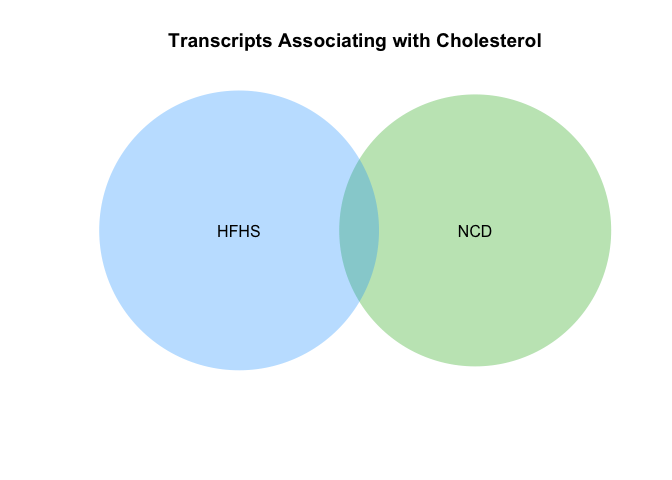
\includegraphics{figures/cholesterol-twas-hf-1.png}

Our analysis identified \textbf{113} nominally significant associations
between expression of genes and adjusted cholesterol levels on a normal
chow diet. Among those, 68 were positively correlated and 68 were
negatively correlated with cholesterol levels.

\hypertarget{twas-modification-by-sex}{%
\subsection{TWAS Modification by Sex}\label{twas-modification-by-sex}}

By modeling the interactions between sex and expression on cholesterol
levels, we identified \textbf{526} genes where the
cholesterol/expression relationship was modified by sex in a nominally
significant manner. This included 14 genes where the relationship was
stronger in males, and 512 where it was stronger in females.

\hypertarget{comparason-with-mouse-gwas}{%
\section{Comparason with mouse GWAS}\label{comparason-with-mouse-gwas}}

\begin{Shaded}
\begin{Highlighting}[]
\NormalTok{chr11.genes }\OtherTok{\textless{}{-}} \FunctionTok{c}\NormalTok{(}\StringTok{\textquotesingle{}Znrf3\textquotesingle{}}\NormalTok{, }\StringTok{\textquotesingle{}Xbp1\textquotesingle{}}\NormalTok{, }\StringTok{\textquotesingle{}Ccdc117\textquotesingle{}}\NormalTok{, }\StringTok{\textquotesingle{}Ankrd36\textquotesingle{}}\NormalTok{, }\StringTok{\textquotesingle{}Mrps24\textquotesingle{}}\NormalTok{, }\StringTok{\textquotesingle{}Urgcp\textquotesingle{}}\NormalTok{, }\StringTok{\textquotesingle{}Dbnl\textquotesingle{}}\NormalTok{, }\StringTok{\textquotesingle{}Pgam2\textquotesingle{}}\NormalTok{, }\StringTok{\textquotesingle{}Polm\textquotesingle{}}\NormalTok{, }\StringTok{\textquotesingle{}Aebp1\textquotesingle{}}\NormalTok{,}\StringTok{\textquotesingle{}Pold2\textquotesingle{}}\NormalTok{, }\StringTok{\textquotesingle{}Myl7\textquotesingle{}}\NormalTok{, }\StringTok{\textquotesingle{}Gck\textquotesingle{}}\NormalTok{, }\StringTok{\textquotesingle{}Ykt6\textquotesingle{}}\NormalTok{, }\StringTok{\textquotesingle{}Camk2b\textquotesingle{}}\NormalTok{, }\StringTok{\textquotesingle{}Nudcd3\textquotesingle{}}\NormalTok{, }\StringTok{\textquotesingle{}A730071L15Rik\textquotesingle{}}\NormalTok{, }\StringTok{\textquotesingle{}Npc1l1\textquotesingle{}}\NormalTok{, }\StringTok{\textquotesingle{}Ddx56\textquotesingle{}}\NormalTok{,}\StringTok{\textquotesingle{}Tmed4\textquotesingle{}}\NormalTok{)}
\NormalTok{genes.of.interest }\OtherTok{\textless{}{-}} \FunctionTok{c}\NormalTok{(}\StringTok{\textquotesingle{}Cyp7a1\textquotesingle{}}\NormalTok{,}\StringTok{\textquotesingle{}Fasn\textquotesingle{}}\NormalTok{,}\StringTok{\textquotesingle{}Ldlr\textquotesingle{}}\NormalTok{,}\StringTok{\textquotesingle{}Hmgcr\textquotesingle{}}\NormalTok{)}
\NormalTok{twas.data.ncd }\SpecialCharTok{\%\textgreater{}\%}
  \FunctionTok{filter}\NormalTok{(symbol }\SpecialCharTok{\%in\%} \FunctionTok{c}\NormalTok{(chr11.genes,genes.of.interest)) }\SpecialCharTok{\%\textgreater{}\%}
  \FunctionTok{kable}\NormalTok{(}\AttributeTok{caption=}\StringTok{"Genes in the chromosome 11 interval with liver expression"}\NormalTok{)}
\end{Highlighting}
\end{Shaded}

\begin{longtable}[]{@{}
  >{\raggedright\arraybackslash}p{(\columnwidth - 14\tabcolsep) * \real{0.2533}}
  >{\raggedright\arraybackslash}p{(\columnwidth - 14\tabcolsep) * \real{0.0800}}
  >{\raggedleft\arraybackslash}p{(\columnwidth - 14\tabcolsep) * \real{0.1200}}
  >{\raggedleft\arraybackslash}p{(\columnwidth - 14\tabcolsep) * \real{0.1333}}
  >{\raggedleft\arraybackslash}p{(\columnwidth - 14\tabcolsep) * \real{0.1333}}
  >{\raggedleft\arraybackslash}p{(\columnwidth - 14\tabcolsep) * \real{0.1067}}
  >{\raggedleft\arraybackslash}p{(\columnwidth - 14\tabcolsep) * \real{0.0800}}
  >{\raggedright\arraybackslash}p{(\columnwidth - 14\tabcolsep) * \real{0.0933}}@{}}
\caption{Genes in the chromosome 11 interval with liver
expression}\tabularnewline
\toprule()
\begin{minipage}[b]{\linewidth}\raggedright
ENSEMBL.ID
\end{minipage} & \begin{minipage}[b]{\linewidth}\raggedright
term
\end{minipage} & \begin{minipage}[b]{\linewidth}\raggedleft
estimate
\end{minipage} & \begin{minipage}[b]{\linewidth}\raggedleft
std.error
\end{minipage} & \begin{minipage}[b]{\linewidth}\raggedleft
statistic
\end{minipage} & \begin{minipage}[b]{\linewidth}\raggedleft
p.value
\end{minipage} & \begin{minipage}[b]{\linewidth}\raggedleft
p.adj
\end{minipage} & \begin{minipage}[b]{\linewidth}\raggedright
symbol
\end{minipage} \\
\midrule()
\endfirsthead
\toprule()
\begin{minipage}[b]{\linewidth}\raggedright
ENSEMBL.ID
\end{minipage} & \begin{minipage}[b]{\linewidth}\raggedright
term
\end{minipage} & \begin{minipage}[b]{\linewidth}\raggedleft
estimate
\end{minipage} & \begin{minipage}[b]{\linewidth}\raggedleft
std.error
\end{minipage} & \begin{minipage}[b]{\linewidth}\raggedleft
statistic
\end{minipage} & \begin{minipage}[b]{\linewidth}\raggedleft
p.value
\end{minipage} & \begin{minipage}[b]{\linewidth}\raggedleft
p.adj
\end{minipage} & \begin{minipage}[b]{\linewidth}\raggedright
symbol
\end{minipage} \\
\midrule()
\endhead
ENSMUSG00000002741 & chol2 & -0.014 & 0.008 & -1.699 & 0.093 & 0.093 &
Ykt6 \\
ENSMUSG00000004394 & chol2 & -0.008 & 0.006 & -1.381 & 0.170 & 0.170 &
Tmed4 \\
ENSMUSG00000041798 & chol2 & 0.055 & 0.053 & 1.027 & 0.307 & 0.307 &
Gck \\
ENSMUSG00000020484 & chol2 & -0.064 & 0.079 & -0.812 & 0.419 & 0.419 &
Xbp1 \\
ENSMUSG00000021670 & chol2 & 0.050 & 0.091 & 0.556 & 0.580 & 0.580 &
Hmgcr \\
ENSMUSG00000028240 & chol2 & -0.049 & 0.138 & -0.355 & 0.724 & 0.724 &
Cyp7a1 \\
ENSMUSG00000032193 & chol2 & -0.004 & 0.043 & -0.090 & 0.928 & 0.928 &
Ldlr \\
ENSMUSG00000025153 & chol2 & 0.050 & 0.636 & 0.078 & 0.938 & 0.938 &
Fasn \\
\bottomrule()
\end{longtable}

\hypertarget{integrated-twas-analysis}{%
\section{Integrated TWAS Analysis}\label{integrated-twas-analysis}}

\begin{Shaded}
\begin{Highlighting}[]
\NormalTok{combined.twas.data }\OtherTok{\textless{}{-}}
  \FunctionTok{full\_join}\NormalTok{(twas.data.ncd, twas.data.hf, }\AttributeTok{by=}\FunctionTok{c}\NormalTok{(}\StringTok{\textquotesingle{}ENSEMBL.ID\textquotesingle{}}\NormalTok{,}\StringTok{\textquotesingle{}term\textquotesingle{}}\NormalTok{,}\StringTok{\textquotesingle{}symbol\textquotesingle{}}\NormalTok{), }\AttributeTok{suffix=}\FunctionTok{c}\NormalTok{(}\StringTok{\textquotesingle{}\_ncd\textquotesingle{}}\NormalTok{,}\StringTok{\textquotesingle{}\_hfd\textquotesingle{}}\NormalTok{))}

\NormalTok{combined.twas.data.all }\OtherTok{\textless{}{-}}
  \FunctionTok{full\_join}\NormalTok{(twas.data.ncd.all, twas.data.hf.all, }\AttributeTok{by=}\FunctionTok{c}\NormalTok{(}\StringTok{\textquotesingle{}ENSEMBL.ID\textquotesingle{}}\NormalTok{,}\StringTok{\textquotesingle{}symbol\textquotesingle{}}\NormalTok{), }\AttributeTok{suffix=}\FunctionTok{c}\NormalTok{(}\StringTok{\textquotesingle{}\_ncd\textquotesingle{}}\NormalTok{,}\StringTok{\textquotesingle{}\_hfd\textquotesingle{}}\NormalTok{))}

\FunctionTok{library}\NormalTok{(ggplot2)}
\FunctionTok{library}\NormalTok{(ggrepel)}
\FunctionTok{ggplot}\NormalTok{(combined.twas.data, }
       \FunctionTok{aes}\NormalTok{(}\AttributeTok{y=}\NormalTok{estimate\_hfd, }\AttributeTok{x=}\NormalTok{estimate\_ncd,}
           \AttributeTok{xmin=}\NormalTok{estimate\_ncd}\SpecialCharTok{{-}}\NormalTok{std.error\_ncd, }\AttributeTok{xmax=}\NormalTok{estimate\_ncd}\SpecialCharTok{+}\NormalTok{std.error\_ncd,}
           \AttributeTok{ymin=}\NormalTok{estimate\_hfd}\SpecialCharTok{{-}}\NormalTok{std.error\_hfd, }\AttributeTok{ymax=}\NormalTok{estimate\_hfd}\SpecialCharTok{+}\NormalTok{std.error\_hfd )) }\SpecialCharTok{+}
  \FunctionTok{geom\_point}\NormalTok{() }\SpecialCharTok{+}
  \CommentTok{\#geom\_errorbar() +}
  \CommentTok{\#geom\_errorbarh() +}
  \FunctionTok{geom\_hline}\NormalTok{(}\AttributeTok{yintercept =} \DecValTok{0}\NormalTok{, }\AttributeTok{lty=}\DecValTok{2}\NormalTok{) }\SpecialCharTok{+}
  \FunctionTok{geom\_vline}\NormalTok{(}\AttributeTok{xintercept =} \DecValTok{0}\NormalTok{, }\AttributeTok{lty=}\DecValTok{2}\NormalTok{) }\SpecialCharTok{+}
  \FunctionTok{geom\_label\_repel}\NormalTok{(}\FunctionTok{aes}\NormalTok{(}\AttributeTok{label=}\NormalTok{symbol),}
                   \AttributeTok{data =} \FunctionTok{subset}\NormalTok{(combined.twas.data, }\FunctionTok{abs}\NormalTok{(estimate\_hfd) }\SpecialCharTok{\textgreater{}} \DecValTok{2}\SpecialCharTok{|}\FunctionTok{abs}\NormalTok{(estimate\_ncd) }\SpecialCharTok{\textgreater{}} \DecValTok{2}\NormalTok{))}
\end{Highlighting}
\end{Shaded}

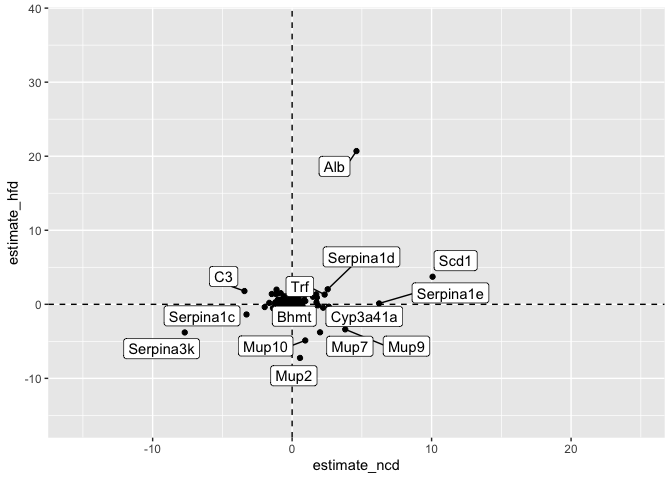
\includegraphics{figures/twas-chol-integrated-1.png}

\begin{Shaded}
\begin{Highlighting}[]
\NormalTok{sig.genes }\OtherTok{\textless{}{-}} \FunctionTok{filter}\NormalTok{(combined.twas.data, p.adj\_ncd}\SpecialCharTok{\textless{}}\FloatTok{0.05}\SpecialCharTok{\&}\NormalTok{p.adj\_hfd}\SpecialCharTok{\textless{}}\FloatTok{0.05}\NormalTok{) }\SpecialCharTok{\%\textgreater{}\%} \FunctionTok{pull}\NormalTok{(symbol)}
\FunctionTok{ggplot}\NormalTok{(combined.twas.data.all }\SpecialCharTok{\%\textgreater{}\%} \FunctionTok{filter}\NormalTok{(symbol }\SpecialCharTok{\%in\%}\NormalTok{ sig.genes), }
       \FunctionTok{aes}\NormalTok{(}\AttributeTok{y=}\NormalTok{estimate.rel\_hfd, }\AttributeTok{x=}\NormalTok{estimate.rel\_ncd,}
           \AttributeTok{xmin=}\NormalTok{estimate.rel\_ncd}\SpecialCharTok{{-}}\NormalTok{std.error.rel\_ncd,}
           \AttributeTok{xmax=}\NormalTok{estimate.rel\_ncd}\SpecialCharTok{+}\NormalTok{std.error.rel\_ncd,}
           \AttributeTok{ymin=}\NormalTok{estimate.rel\_hfd}\SpecialCharTok{{-}}\NormalTok{std.error.rel\_hfd,}
           \AttributeTok{ymax=}\NormalTok{estimate.rel\_hfd}\SpecialCharTok{+}\NormalTok{std.error.rel\_hfd )) }\SpecialCharTok{+}
  \FunctionTok{geom\_point}\NormalTok{() }\SpecialCharTok{+}
  \FunctionTok{geom\_errorbar}\NormalTok{() }\SpecialCharTok{+}
  \FunctionTok{geom\_errorbarh}\NormalTok{() }\SpecialCharTok{+}
  \FunctionTok{geom\_hline}\NormalTok{(}\AttributeTok{yintercept =} \DecValTok{0}\NormalTok{, }\AttributeTok{lty=}\DecValTok{2}\NormalTok{) }\SpecialCharTok{+}
  \FunctionTok{geom\_vline}\NormalTok{(}\AttributeTok{xintercept =} \DecValTok{0}\NormalTok{, }\AttributeTok{lty=}\DecValTok{2}\NormalTok{) }\SpecialCharTok{+}
  \FunctionTok{geom\_text\_repel}\NormalTok{(}\FunctionTok{aes}\NormalTok{(}\AttributeTok{label=}\NormalTok{symbol))}
\end{Highlighting}
\end{Shaded}

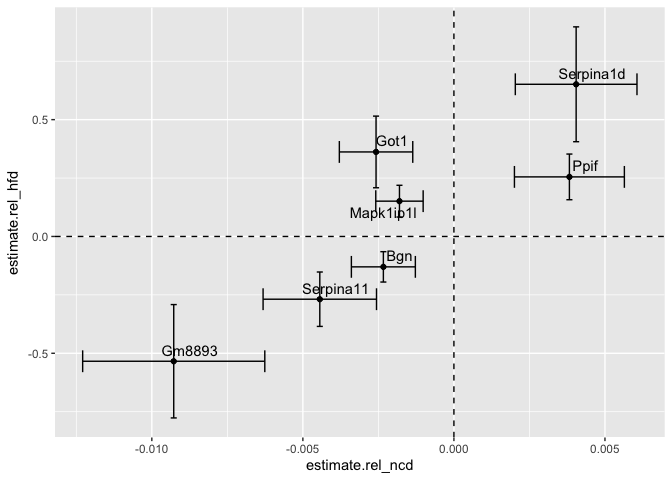
\includegraphics{figures/twas-chol-integrated-2.png}

\begin{Shaded}
\begin{Highlighting}[]
\NormalTok{sig.genes }\OtherTok{\textless{}{-}} \FunctionTok{filter}\NormalTok{(combined.twas.data, p.adj\_ncd}\SpecialCharTok{\textless{}}\FloatTok{0.05}\SpecialCharTok{|}\NormalTok{p.adj\_hfd}\SpecialCharTok{\textless{}}\FloatTok{0.05}\NormalTok{) }\SpecialCharTok{\%\textgreater{}\%} \FunctionTok{pull}\NormalTok{(symbol)}
\FunctionTok{ggplot}\NormalTok{(combined.twas.data.all }\SpecialCharTok{\%\textgreater{}\%} \FunctionTok{filter}\NormalTok{(symbol }\SpecialCharTok{\%in\%}\NormalTok{ sig.genes), }
       \FunctionTok{aes}\NormalTok{(}\AttributeTok{y=}\NormalTok{estimate.rel\_hfd, }\AttributeTok{x=}\NormalTok{estimate.rel\_ncd,}
           \AttributeTok{xmin=}\NormalTok{estimate.rel\_ncd}\SpecialCharTok{{-}}\NormalTok{std.error.rel\_ncd,}
           \AttributeTok{xmax=}\NormalTok{estimate.rel\_ncd}\SpecialCharTok{+}\NormalTok{std.error.rel\_ncd,}
           \AttributeTok{ymin=}\NormalTok{estimate.rel\_hfd}\SpecialCharTok{{-}}\NormalTok{std.error.rel\_hfd,}
           \AttributeTok{ymax=}\NormalTok{estimate.rel\_hfd}\SpecialCharTok{+}\NormalTok{std.error.rel\_hfd )) }\SpecialCharTok{+}
  \FunctionTok{geom\_point}\NormalTok{() }\SpecialCharTok{+}
  \FunctionTok{geom\_errorbar}\NormalTok{() }\SpecialCharTok{+}
  \FunctionTok{geom\_errorbarh}\NormalTok{() }\SpecialCharTok{+}
  \FunctionTok{geom\_smooth}\NormalTok{() }\SpecialCharTok{+}
  \FunctionTok{geom\_hline}\NormalTok{(}\AttributeTok{yintercept =} \DecValTok{0}\NormalTok{, }\AttributeTok{lty=}\DecValTok{2}\NormalTok{) }\SpecialCharTok{+}
  \FunctionTok{geom\_vline}\NormalTok{(}\AttributeTok{xintercept =} \DecValTok{0}\NormalTok{, }\AttributeTok{lty=}\DecValTok{2}\NormalTok{) }\SpecialCharTok{+}
  \FunctionTok{xlim}\NormalTok{(}\SpecialCharTok{{-}}\FloatTok{0.03}\NormalTok{,}\FloatTok{0.03}\NormalTok{) }\SpecialCharTok{+}
  \FunctionTok{ylim}\NormalTok{(}\SpecialCharTok{{-}}\FloatTok{0.03}\NormalTok{,}\FloatTok{0.03}\NormalTok{) }\SpecialCharTok{+}
  \FunctionTok{geom\_text\_repel}\NormalTok{(}\FunctionTok{aes}\NormalTok{(}\AttributeTok{label=}\NormalTok{symbol)) }\SpecialCharTok{+}
  \FunctionTok{labs}\NormalTok{(}\AttributeTok{y=}\StringTok{"On HFHS Diet (beta)"}\NormalTok{,}
       \AttributeTok{x=}\StringTok{"On NCD Diet (beta)"}\NormalTok{,}
       \AttributeTok{title=}\StringTok{"Associations of Liver Transcripts with Cholesterol"}\NormalTok{,}
       \AttributeTok{subtitle=}\StringTok{"Significant for at least one diet"}\NormalTok{)}
\end{Highlighting}
\end{Shaded}

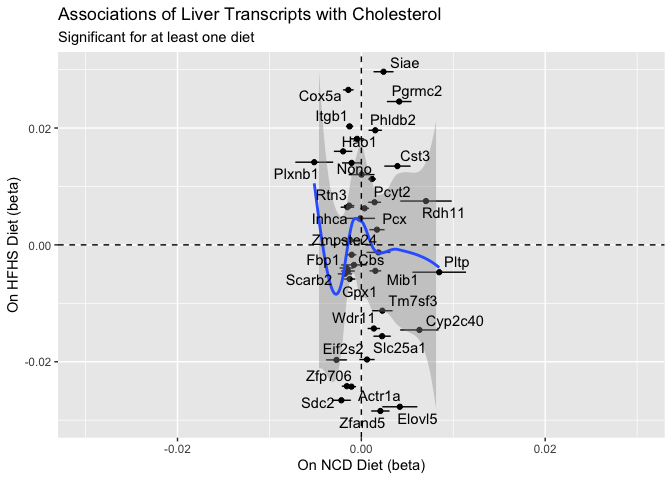
\includegraphics{figures/twas-chol-integrated-3.png}

\begin{Shaded}
\begin{Highlighting}[]
\NormalTok{cutoff }\OtherTok{\textless{}{-}} \SpecialCharTok{{-}}\FunctionTok{log10}\NormalTok{(}\FloatTok{0.05}\NormalTok{)}
\FunctionTok{ggplot}\NormalTok{(combined.twas.data, }
       \FunctionTok{aes}\NormalTok{(}\AttributeTok{y=}\SpecialCharTok{{-}}\FunctionTok{log10}\NormalTok{(p.adj\_hfd), }\AttributeTok{x=}\SpecialCharTok{{-}}\FunctionTok{log10}\NormalTok{(p.adj\_ncd) )) }\SpecialCharTok{+}
  \FunctionTok{geom\_point}\NormalTok{() }\SpecialCharTok{+}
  \CommentTok{\#geom\_errorbar() +}
  \CommentTok{\#geom\_errorbarh() +}
  \FunctionTok{geom\_hline}\NormalTok{(}\AttributeTok{yintercept =} \SpecialCharTok{{-}}\FunctionTok{log10}\NormalTok{(}\FloatTok{0.05}\NormalTok{), }\AttributeTok{lty=}\DecValTok{2}\NormalTok{) }\SpecialCharTok{+}
  \FunctionTok{geom\_vline}\NormalTok{(}\AttributeTok{xintercept =} \SpecialCharTok{{-}}\FunctionTok{log10}\NormalTok{(}\FloatTok{0.05}\NormalTok{), }\AttributeTok{lty=}\DecValTok{2}\NormalTok{) }\SpecialCharTok{+}
  \FunctionTok{geom\_text\_repel}\NormalTok{(}\FunctionTok{aes}\NormalTok{(}\AttributeTok{label=}\NormalTok{symbol),}
                   \AttributeTok{data =} \FunctionTok{subset}\NormalTok{(combined.twas.data, }\SpecialCharTok{{-}}\FunctionTok{log10}\NormalTok{(p.adj\_hfd) }\SpecialCharTok{\textgreater{}}\NormalTok{ cutoff}\SpecialCharTok{|{-}}\FunctionTok{log10}\NormalTok{(p.adj\_ncd) }\SpecialCharTok{\textgreater{}}\NormalTok{ cutoff)) }\SpecialCharTok{+}
  \FunctionTok{labs}\NormalTok{(}\AttributeTok{y=}\StringTok{"On HFHS Diet (log10 q{-}value)"}\NormalTok{,}
       \AttributeTok{x=}\StringTok{"On NCD Diet (log10 q{-}value)"}\NormalTok{,}
       \AttributeTok{title=}\StringTok{"Associations of Liver Transcripts with Cholesterol"}\NormalTok{) }\SpecialCharTok{+}
  \FunctionTok{theme\_classic}\NormalTok{() }\SpecialCharTok{+}
  \FunctionTok{theme}\NormalTok{(}\AttributeTok{text=}\FunctionTok{element\_text}\NormalTok{(}\AttributeTok{size=}\DecValTok{16}\NormalTok{))}
\end{Highlighting}
\end{Shaded}

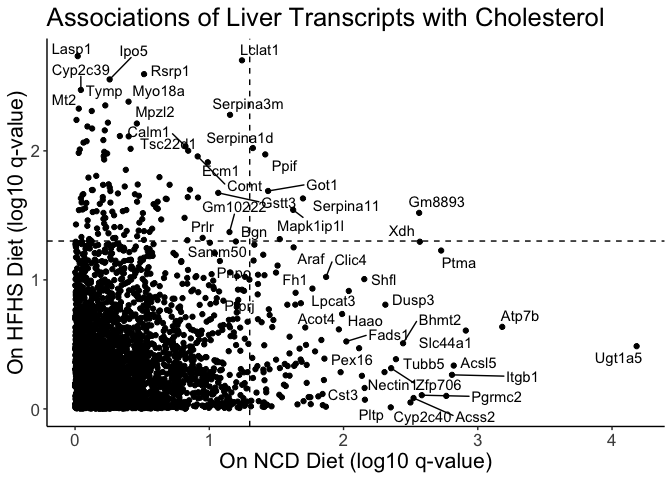
\includegraphics{figures/twas-chol-integrated-4.png} \# Comparason with
human GWAS

Downloaded human cholesterol associated alleles from
\url{https://t2d.hugeamp.org/phenotype.html?phenotype=CHOL}

```\{ chol-human-gwas\} gwas.filename \textless-
`cholesterol-associations.csv' gwas.data \textless-
read\_csv(gwas.filename) \%\textgreater\% mutate(Symbol=gsub(`.\{2\}\$',
'\,', nearest)) \%\textgreater\% mutate(Symbol=gsub(``\^{}.\{0,2\}'',
``\,``,Symbol)) \#removes first and last characters

library(biomaRt) human = useMart(``ensembl'', dataset =
``hsapiens\_gene\_ensembl'') mouse = useMart(``ensembl'', dataset =
``mmusculus\_gene\_ensembl'')

mapping.data \textless- getLDS(attributes = c(``hgnc\_symbol''), filters
= ``hgnc\_symbol'', values = gwas.data\$Symbol , mart = human,
attributesL = c(``mgi\_symbol''), martL = mouse, uniqueRows=T)

gwas.data \textless- full\_join(gwas.data, mapping.data,
by=c(`Symbol'=`HGNC.symbol')) \%\textgreater\%
dplyr::filter(!(is.na(MGI.symbol)))

\#are gwas alleles enriched in correlation analyses

sig.twas.data \textless- filter(twas.data, p.value\textless0.05)
\#sig.twas.data\(symbol %in% gwas.data
\)MGI.symbol \%\textgreater\% table

combined.twas.data \%\textgreater\% filter(symbol \%in\%
gwas.data\$MGI.symbol) \%\textgreater\% arrange(p.value)
\%\textgreater\% head \%\textgreater\% kable(caption=``Most significant
TWAS association hits that are also nearby GWAS hits'')

\#checked if a TWAS was a GWAS hit twas.data.matched \textless-
combined.twas.data \%\textgreater\% mutate(hGWAS.match=symbol \%in\%
gwas.data\$MGI.symbol)

with(twas.data.matched, table(hGWAS.match,p.value\textless0.05))
\%\textgreater\% fisher.test() \%\textgreater\% tidy \%\textgreater\%
kable(caption=`Fisher test for enrichment of GWAS hits in liver TWAS
genes')

glm(hGWAS.match\textasciitilde p.value, data=twas.data.matched,
family=`binomial') \%\textgreater\% tidy \%\textgreater\%
kable(caption=``Logistic regression of TWAS values against likilihood of
a GWAS hit.'')

\begin{verbatim}

# Pathway Analyses for NCD


```r
twas.list <- twas.data.ncd %>% arrange(-estimate) %>% pull(estimate)
names(twas.list) <- twas.data.ncd %>% arrange(-estimate) %>% pull(symbol)
twas.list <- sort(twas.list, decreasing = TRUE)
#twas.list <- twas.list[!(is.na(names(twas.list)))]


library(clusterProfiler)
go.twas.bp <- gseGO(geneList=twas.list, 
               ont="BP", 
               keyType='SYMBOL',
               OrgDb=org.Mm.eg.db, 
               pvalueCutoff=0.25,
               verbose=T,
               by='fgsea',
               eps=1E-25)

#enrichement
twas.data.ncd %>% 
  filter(p.value<0.05) %>%
  pull(symbol) ->
  twas.sig

go.twas.bp.enrich <- enrichGO(gene=twas.sig, 
               ont="BP", 
               keyType='SYMBOL',
               OrgDb=org.Mm.eg.db, 
               pvalueCutoff=0.05)

go.twas.bp.enrich.simpl <- simplify(go.twas.bp.enrich,
                             cutoff=0.7, 
                             by="p.adjust",
                             select_fun=min)

library(enrichplot)

dotplot(go.twas.bp.enrich.simpl, 
        showCategory=50,
        color='pvalue',
        font.size=8)
\end{verbatim}

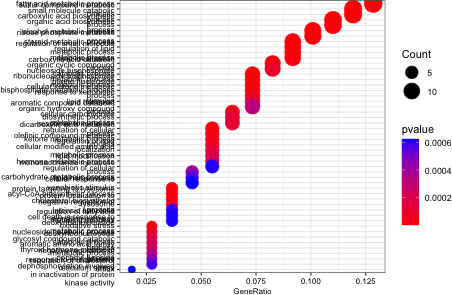
\includegraphics{figures/twas-go-ncd-1.png}

\begin{Shaded}
\begin{Highlighting}[]
\FunctionTok{barplot}\NormalTok{(go.twas.bp.enrich.simpl,}\AttributeTok{font.size=}\DecValTok{8}\NormalTok{)}
\end{Highlighting}
\end{Shaded}

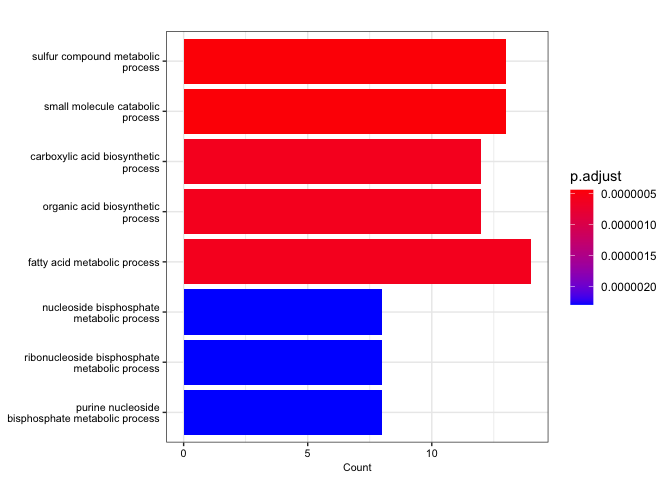
\includegraphics{figures/twas-go-ncd-2.png}

\begin{Shaded}
\begin{Highlighting}[]
\FunctionTok{cnetplot}\NormalTok{(go.twas.bp.enrich.simpl, }
         \AttributeTok{showCategory=}\DecValTok{100}\NormalTok{,}
         \AttributeTok{node\_label=}\StringTok{"gene"}\NormalTok{,}
         \AttributeTok{cex\_label\_gene=}\FloatTok{0.5}\NormalTok{)}
\end{Highlighting}
\end{Shaded}

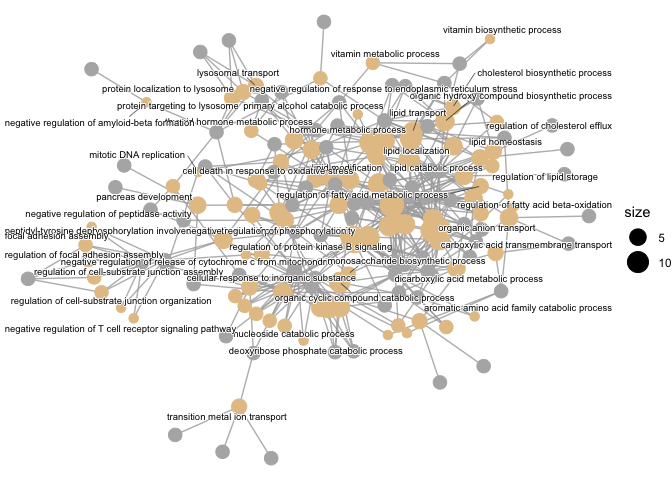
\includegraphics{figures/twas-go-ncd-3.png}

\begin{Shaded}
\begin{Highlighting}[]
\FunctionTok{cnetplot}\NormalTok{(go.twas.bp.enrich.simpl, }
         \AttributeTok{showCategory=}\DecValTok{100}\NormalTok{,}
         \AttributeTok{node\_label=}\StringTok{"category"}\NormalTok{,}
         \AttributeTok{cex\_label\_category=}\FloatTok{0.5}\NormalTok{)}
\end{Highlighting}
\end{Shaded}

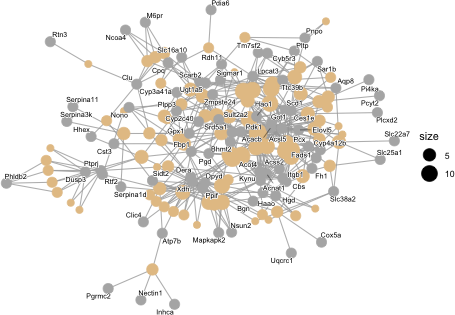
\includegraphics{figures/twas-go-ncd-4.png}

\begin{Shaded}
\begin{Highlighting}[]
\FunctionTok{heatplot}\NormalTok{(go.twas.bp.enrich.simpl)}
\end{Highlighting}
\end{Shaded}

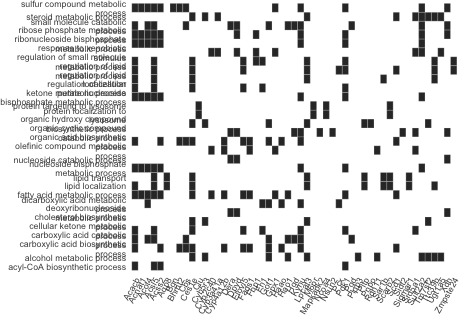
\includegraphics{figures/twas-go-ncd-5.png}

\begin{Shaded}
\begin{Highlighting}[]
\FunctionTok{library}\NormalTok{(ggupset)}
\FunctionTok{upsetplot}\NormalTok{(go.twas.bp.enrich.simpl)}
\end{Highlighting}
\end{Shaded}

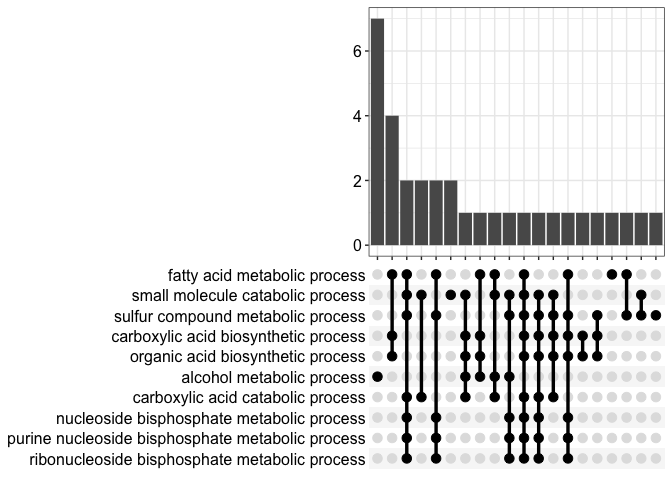
\includegraphics{figures/twas-go-ncd-6.png}

\begin{Shaded}
\begin{Highlighting}[]
\FunctionTok{dotplot}\NormalTok{(go.twas.bp.enrich.simpl, }\AttributeTok{showCategory=}\DecValTok{30}\NormalTok{)}
\end{Highlighting}
\end{Shaded}

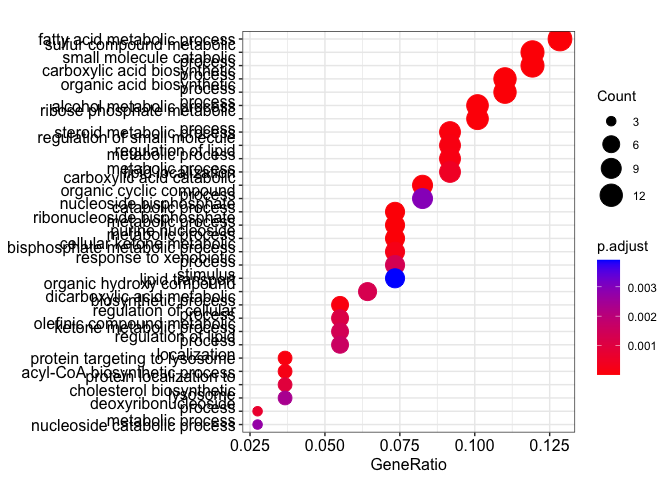
\includegraphics{figures/twas-go-ncd-7.png}

\begin{Shaded}
\begin{Highlighting}[]
\FunctionTok{heatplot}\NormalTok{(go.twas.bp.enrich.simpl, }\AttributeTok{foldChange=}\NormalTok{twas.list)}
\end{Highlighting}
\end{Shaded}

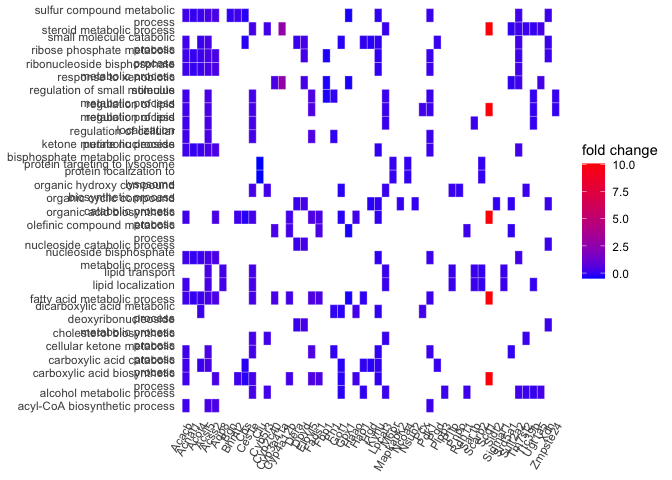
\includegraphics{figures/twas-go-ncd-8.png}

\begin{Shaded}
\begin{Highlighting}[]
\FunctionTok{upsetplot}\NormalTok{(go.twas.bp.enrich.simpl)}
\end{Highlighting}
\end{Shaded}

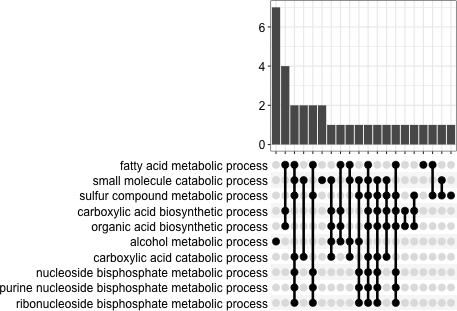
\includegraphics{figures/twas-go-ncd-9.png}

\begin{Shaded}
\begin{Highlighting}[]
\FunctionTok{as.data.frame}\NormalTok{(go.twas.bp) }\SpecialCharTok{\%\textgreater{}\%} \FunctionTok{select}\NormalTok{(}\StringTok{"Description"}\NormalTok{,}\StringTok{"setSize"}\NormalTok{,}\StringTok{"enrichmentScore"}\NormalTok{,}\StringTok{"NES"}\NormalTok{,}\StringTok{"pvalue"}\NormalTok{,}\StringTok{"p.adjust"}\NormalTok{) }\SpecialCharTok{\%\textgreater{}\%}
  \FunctionTok{kable}\NormalTok{(}\AttributeTok{caption=}\StringTok{"NCD GO BP Analysis of TWAS Associations from GSEA"}\NormalTok{)}
\end{Highlighting}
\end{Shaded}

\begin{longtable}[]{@{}lrrrrr@{}}
\caption{NCD GO BP Analysis of TWAS Associations from
GSEA}\tabularnewline
\toprule()
Description & setSize & enrichmentScore & NES & pvalue & p.adjust \\
\midrule()
\endfirsthead
\toprule()
Description & setSize & enrichmentScore & NES & pvalue & p.adjust \\
\midrule()
\endhead
\bottomrule()
\end{longtable}

\begin{Shaded}
\begin{Highlighting}[]
\FunctionTok{as.data.frame}\NormalTok{(go.twas.bp) }\SpecialCharTok{\%\textgreater{}\%}
  \FunctionTok{write\_csv}\NormalTok{(}\AttributeTok{file=}\StringTok{"NCD TWAS GO{-}BP GSEA.csv"}\NormalTok{)}

\FunctionTok{as.data.frame}\NormalTok{(go.twas.bp.enrich.simpl) }\SpecialCharTok{\%\textgreater{}\%} \FunctionTok{select}\NormalTok{(}\StringTok{"Description"}\NormalTok{,}\StringTok{"GeneRatio"}\NormalTok{,}\StringTok{"Count"}\NormalTok{,}\StringTok{"pvalue"}\NormalTok{,}\StringTok{"p.adjust"}\NormalTok{) }\SpecialCharTok{\%\textgreater{}\%} 
  \FunctionTok{kable}\NormalTok{(}\AttributeTok{caption=}\StringTok{"NCD GO BP Analysis of TWAS Associations from Enrichment"}\NormalTok{)}
\end{Highlighting}
\end{Shaded}

\begin{longtable}[]{@{}
  >{\raggedright\arraybackslash}p{(\columnwidth - 10\tabcolsep) * \real{0.0840}}
  >{\raggedright\arraybackslash}p{(\columnwidth - 10\tabcolsep) * \real{0.6718}}
  >{\raggedright\arraybackslash}p{(\columnwidth - 10\tabcolsep) * \real{0.0763}}
  >{\raggedleft\arraybackslash}p{(\columnwidth - 10\tabcolsep) * \real{0.0458}}
  >{\raggedleft\arraybackslash}p{(\columnwidth - 10\tabcolsep) * \real{0.0534}}
  >{\raggedleft\arraybackslash}p{(\columnwidth - 10\tabcolsep) * \real{0.0687}}@{}}
\caption{NCD GO BP Analysis of TWAS Associations from
Enrichment}\tabularnewline
\toprule()
\begin{minipage}[b]{\linewidth}\raggedright
\end{minipage} & \begin{minipage}[b]{\linewidth}\raggedright
Description
\end{minipage} & \begin{minipage}[b]{\linewidth}\raggedright
GeneRatio
\end{minipage} & \begin{minipage}[b]{\linewidth}\raggedleft
Count
\end{minipage} & \begin{minipage}[b]{\linewidth}\raggedleft
pvalue
\end{minipage} & \begin{minipage}[b]{\linewidth}\raggedleft
p.adjust
\end{minipage} \\
\midrule()
\endfirsthead
\toprule()
\begin{minipage}[b]{\linewidth}\raggedright
\end{minipage} & \begin{minipage}[b]{\linewidth}\raggedright
Description
\end{minipage} & \begin{minipage}[b]{\linewidth}\raggedright
GeneRatio
\end{minipage} & \begin{minipage}[b]{\linewidth}\raggedleft
Count
\end{minipage} & \begin{minipage}[b]{\linewidth}\raggedleft
pvalue
\end{minipage} & \begin{minipage}[b]{\linewidth}\raggedleft
p.adjust
\end{minipage} \\
\midrule()
\endhead
\url{GO:0006790} & sulfur compound metabolic process & 13/109 & 13 &
0.000 & 0.000 \\
\url{GO:0044282} & small molecule catabolic process & 13/109 & 13 &
0.000 & 0.000 \\
\url{GO:0046394} & carboxylic acid biosynthetic process & 12/109 & 12 &
0.000 & 0.000 \\
\url{GO:0016053} & organic acid biosynthetic process & 12/109 & 12 &
0.000 & 0.000 \\
\url{GO:0006631} & fatty acid metabolic process & 14/109 & 14 & 0.000 &
0.000 \\
\url{GO:0033865} & nucleoside bisphosphate metabolic process & 8/109 & 8
& 0.000 & 0.000 \\
\url{GO:0033875} & ribonucleoside bisphosphate metabolic process & 8/109
& 8 & 0.000 & 0.000 \\
\url{GO:0034032} & purine nucleoside bisphosphate metabolic process &
8/109 & 8 & 0.000 & 0.000 \\
\url{GO:0006066} & alcohol metabolic process & 11/109 & 11 & 0.000 &
0.000 \\
\url{GO:0046395} & carboxylic acid catabolic process & 9/109 & 9 & 0.000
& 0.000 \\
\url{GO:0019693} & ribose phosphate metabolic process & 11/109 & 11 &
0.000 & 0.000 \\
\url{GO:0008202} & steroid metabolic process & 10/109 & 10 & 0.000 &
0.000 \\
\url{GO:0043648} & dicarboxylic acid metabolic process & 6/109 & 6 &
0.000 & 0.000 \\
\url{GO:0006622} & protein targeting to lysosome & 4/109 & 4 & 0.000 &
0.000 \\
\url{GO:0062012} & regulation of small molecule metabolic process &
10/109 & 10 & 0.000 & 0.000 \\
\url{GO:0019216} & regulation of lipid metabolic process & 10/109 & 10 &
0.000 & 0.000 \\
\url{GO:0071616} & acyl-CoA biosynthetic process & 4/109 & 4 & 0.000 &
0.000 \\
\url{GO:0042180} & cellular ketone metabolic process & 8/109 & 8 & 0.000
& 0.000 \\
\url{GO:0010876} & lipid localization & 10/109 & 10 & 0.000 & 0.000 \\
\url{GO:0009120} & deoxyribonucleoside metabolic process & 3/109 & 3 &
0.000 & 0.001 \\
\url{GO:0061462} & protein localization to lysosome & 4/109 & 4 & 0.000
& 0.001 \\
\url{GO:0010565} & regulation of cellular ketone metabolic process &
6/109 & 6 & 0.000 & 0.001 \\
\url{GO:1901617} & organic hydroxy compound biosynthetic process & 7/109
& 7 & 0.000 & 0.001 \\
\url{GO:0009410} & response to xenobiotic stimulus & 8/109 & 8 & 0.000 &
0.001 \\
\url{GO:0120254} & olefinic compound metabolic process & 6/109 & 6 &
0.000 & 0.001 \\
\url{GO:1905952} & regulation of lipid localization & 6/109 & 6 & 0.000
& 0.002 \\
\url{GO:0006695} & cholesterol biosynthetic process & 4/109 & 4 & 0.000
& 0.002 \\
\url{GO:0009164} & nucleoside catabolic process & 3/109 & 3 & 0.000 &
0.003 \\
\url{GO:1901361} & organic cyclic compound catabolic process & 9/109 & 9
& 0.000 & 0.003 \\
\url{GO:0006869} & lipid transport & 8/109 & 8 & 0.000 & 0.004 \\
\url{GO:0006575} & cellular modified amino acid metabolic process &
6/109 & 6 & 0.000 & 0.004 \\
\url{GO:0044262} & cellular carbohydrate metabolic process & 7/109 & 7 &
0.000 & 0.004 \\
\url{GO:0010038} & response to metal ion & 7/109 & 7 & 0.000 & 0.004 \\
\url{GO:0009264} & deoxyribonucleotide catabolic process & 3/109 & 3 &
0.000 & 0.004 \\
\url{GO:0030258} & lipid modification & 6/109 & 6 & 0.000 & 0.005 \\
\url{GO:1901658} & glycosyl compound catabolic process & 3/109 & 3 &
0.000 & 0.005 \\
\url{GO:0042445} & hormone metabolic process & 6/109 & 6 & 0.000 &
0.005 \\
\url{GO:0009072} & aromatic amino acid family metabolic process & 3/109
& 3 & 0.000 & 0.006 \\
\url{GO:0042403} & thyroid hormone metabolic process & 3/109 & 3 & 0.000
& 0.008 \\
\url{GO:0019439} & aromatic compound catabolic process & 8/109 & 8 &
0.000 & 0.008 \\
\url{GO:0010675} & regulation of cellular carbohydrate metabolic process
& 5/109 & 5 & 0.000 & 0.010 \\
\url{GO:1903573} & negative regulation of response to endoplasmic
reticulum stress & 3/109 & 3 & 0.000 & 0.011 \\
\url{GO:0055088} & lipid homeostasis & 5/109 & 5 & 0.001 & 0.013 \\
\url{GO:0010874} & regulation of cholesterol efflux & 3/109 & 3 & 0.001
& 0.013 \\
\url{GO:2001243} & negative regulation of intrinsic apoptotic signaling
pathway & 4/109 & 4 & 0.001 & 0.013 \\
\url{GO:0005996} & monosaccharide metabolic process & 6/109 & 6 & 0.001
& 0.013 \\
\url{GO:0019217} & regulation of fatty acid metabolic process & 4/109 &
4 & 0.001 & 0.013 \\
\url{GO:0036473} & cell death in response to oxidative stress & 4/109 &
4 & 0.001 & 0.013 \\
\url{GO:0071466} & cellular response to xenobiotic stimulus & 5/109 & 5
& 0.001 & 0.013 \\
\url{GO:1990264} & peptidyl-tyrosine dephosphorylation involved in
inactivation of protein kinase activity & 2/109 & 2 & 0.001 & 0.013 \\
\url{GO:0008631} & intrinsic apoptotic signaling pathway in response to
oxidative stress & 3/109 & 3 & 0.001 & 0.014 \\
\url{GO:0000041} & transition metal ion transport & 4/109 & 4 & 0.001 &
0.016 \\
\url{GO:0034310} & primary alcohol catabolic process & 2/109 & 2 & 0.001
& 0.017 \\
\url{GO:0007041} & lysosomal transport & 4/109 & 4 & 0.001 & 0.019 \\
\url{GO:0010883} & regulation of lipid storage & 3/109 & 3 & 0.001 &
0.020 \\
\url{GO:0044270} & cellular nitrogen compound catabolic process & 7/109
& 7 & 0.001 & 0.021 \\
\url{GO:0046700} & heterocycle catabolic process & 7/109 & 7 & 0.001 &
0.021 \\
\url{GO:1902969} & mitotic DNA replication & 2/109 & 2 & 0.001 &
0.021 \\
\url{GO:0016042} & lipid catabolic process & 6/109 & 6 & 0.002 &
0.025 \\
\url{GO:0008654} & phospholipid biosynthetic process & 5/109 & 5 & 0.002
& 0.025 \\
\url{GO:0009074} & aromatic amino acid family catabolic process & 2/109
& 2 & 0.002 & 0.025 \\
\url{GO:0051893} & regulation of focal adhesion assembly & 3/109 & 3 &
0.002 & 0.027 \\
\url{GO:0090109} & regulation of cell-substrate junction assembly &
3/109 & 3 & 0.002 & 0.027 \\
\url{GO:0071243} & cellular response to arsenic-containing substance &
2/109 & 2 & 0.002 & 0.027 \\
\url{GO:1905039} & carboxylic acid transmembrane transport & 4/109 & 4 &
0.002 & 0.028 \\
\url{GO:0016052} & carbohydrate catabolic process & 4/109 & 4 & 0.002 &
0.028 \\
\url{GO:0071241} & cellular response to inorganic substance & 5/109 & 5
& 0.002 & 0.030 \\
\url{GO:0007584} & response to nutrient & 3/109 & 3 & 0.002 & 0.030 \\
\url{GO:0015711} & organic anion transport & 6/109 & 6 & 0.002 &
0.031 \\
\url{GO:0150116} & regulation of cell-substrate junction organization &
3/109 & 3 & 0.002 & 0.031 \\
\url{GO:0009110} & vitamin biosynthetic process & 2/109 & 2 & 0.003 &
0.033 \\
\url{GO:1902430} & negative regulation of amyloid-beta formation & 2/109
& 2 & 0.003 & 0.033 \\
\url{GO:0071404} & cellular response to low-density lipoprotein particle
stimulus & 2/109 & 2 & 0.003 & 0.038 \\
\url{GO:1901657} & glycosyl compound metabolic process & 3/109 & 3 &
0.003 & 0.038 \\
\url{GO:0010466} & negative regulation of peptidase activity & 5/109 & 5
& 0.003 & 0.039 \\
\url{GO:0031998} & regulation of fatty acid beta-oxidation & 2/109 & 2 &
0.003 & 0.040 \\
\url{GO:0090201} & negative regulation of release of cytochrome c from
mitochondria & 2/109 & 2 & 0.003 & 0.040 \\
\url{GO:0009060} & aerobic respiration & 4/109 & 4 & 0.004 & 0.041 \\
\url{GO:0006766} & vitamin metabolic process & 3/109 & 3 & 0.004 &
0.044 \\
\url{GO:0050860} & negative regulation of T cell receptor signaling
pathway & 2/109 & 2 & 0.004 & 0.044 \\
\url{GO:0042326} & negative regulation of phosphorylation & 6/109 & 6 &
0.004 & 0.045 \\
\url{GO:0048041} & focal adhesion assembly & 3/109 & 3 & 0.004 &
0.045 \\
\url{GO:0046386} & deoxyribose phosphate catabolic process & 2/109 & 2 &
0.004 & 0.045 \\
\url{GO:0046685} & response to arsenic-containing substance & 2/109 & 2
& 0.004 & 0.045 \\
\url{GO:0051896} & regulation of protein kinase B signaling & 4/109 & 4
& 0.005 & 0.047 \\
\url{GO:0006979} & response to oxidative stress & 6/109 & 6 & 0.005 &
0.047 \\
\url{GO:0031016} & pancreas development & 3/109 & 3 & 0.005 & 0.049 \\
\url{GO:0046364} & monosaccharide biosynthetic process & 3/109 & 3 &
0.005 & 0.049 \\
\url{GO:0042059} & negative regulation of epidermal growth factor
receptor signaling pathway & 2/109 & 2 & 0.005 & 0.049 \\
\bottomrule()
\end{longtable}

\begin{Shaded}
\begin{Highlighting}[]
\FunctionTok{as.data.frame}\NormalTok{(go.twas.bp.enrich.simpl) }\SpecialCharTok{\%\textgreater{}\%}
  \FunctionTok{write\_csv}\NormalTok{(}\AttributeTok{file=}\StringTok{"NCD TWAS GO{-}BP Enrichment.csv"}\NormalTok{)}

\NormalTok{steroid.enrichment }\OtherTok{\textless{}{-}} \FunctionTok{as.data.frame}\NormalTok{(go.twas.bp) }\SpecialCharTok{\%\textgreater{}\%} \FunctionTok{filter}\NormalTok{(ID}\SpecialCharTok{==}\StringTok{\textquotesingle{}GO:0016126\textquotesingle{}}\NormalTok{)}
\end{Highlighting}
\end{Shaded}

\hypertarget{pathway-analyses-for-hfd}{%
\section{Pathway Analyses for HFD}\label{pathway-analyses-for-hfd}}

\begin{Shaded}
\begin{Highlighting}[]
\NormalTok{twas.list }\OtherTok{\textless{}{-}}\NormalTok{ twas.data.hf }\SpecialCharTok{\%\textgreater{}\%} \FunctionTok{arrange}\NormalTok{(}\SpecialCharTok{{-}}\NormalTok{estimate) }\SpecialCharTok{\%\textgreater{}\%} \FunctionTok{pull}\NormalTok{(estimate)}
\FunctionTok{names}\NormalTok{(twas.list) }\OtherTok{\textless{}{-}}\NormalTok{ twas.data.hf }\SpecialCharTok{\%\textgreater{}\%} \FunctionTok{arrange}\NormalTok{(}\SpecialCharTok{{-}}\NormalTok{estimate) }\SpecialCharTok{\%\textgreater{}\%} \FunctionTok{pull}\NormalTok{(symbol)}
\NormalTok{twas.list }\OtherTok{\textless{}{-}} \FunctionTok{sort}\NormalTok{(twas.list, }\AttributeTok{decreasing =} \ConstantTok{TRUE}\NormalTok{)}
\CommentTok{\#twas.list \textless{}{-} twas.list[!(is.na(names(twas.list)))]}


\FunctionTok{library}\NormalTok{(clusterProfiler)}
\NormalTok{go.twas.bp }\OtherTok{\textless{}{-}} \FunctionTok{gseGO}\NormalTok{(}\AttributeTok{geneList=}\NormalTok{twas.list, }
               \AttributeTok{ont=}\StringTok{"BP"}\NormalTok{, }
               \AttributeTok{keyType=}\StringTok{\textquotesingle{}SYMBOL\textquotesingle{}}\NormalTok{,}
               \AttributeTok{OrgDb=}\NormalTok{org.Mm.eg.db, }
               \AttributeTok{pvalueCutoff=}\FloatTok{0.25}\NormalTok{,}
               \AttributeTok{verbose=}\NormalTok{T,}
               \AttributeTok{by=}\StringTok{\textquotesingle{}fgsea\textquotesingle{}}\NormalTok{,}
               \AttributeTok{eps=}\FloatTok{1E{-}25}\NormalTok{)}

\CommentTok{\#enrichement}
\NormalTok{twas.data.hf }\SpecialCharTok{\%\textgreater{}\%} 
  \FunctionTok{filter}\NormalTok{(p.value}\SpecialCharTok{\textless{}}\FloatTok{0.05}\NormalTok{) }\SpecialCharTok{\%\textgreater{}\%}
  \FunctionTok{pull}\NormalTok{(symbol) }\OtherTok{{-}\textgreater{}}
\NormalTok{  twas.sig}

\NormalTok{go.twas.bp.enrich }\OtherTok{\textless{}{-}} \FunctionTok{enrichGO}\NormalTok{(}\AttributeTok{gene=}\NormalTok{twas.sig, }
               \AttributeTok{ont=}\StringTok{"BP"}\NormalTok{, }
               \AttributeTok{keyType=}\StringTok{\textquotesingle{}SYMBOL\textquotesingle{}}\NormalTok{,}
               \AttributeTok{OrgDb=}\NormalTok{org.Mm.eg.db, }
               \AttributeTok{pvalueCutoff=}\FloatTok{0.05}\NormalTok{)}

\NormalTok{go.twas.bp.enrich.simpl }\OtherTok{\textless{}{-}} \FunctionTok{simplify}\NormalTok{(go.twas.bp.enrich,}
                             \AttributeTok{cutoff=}\FloatTok{0.7}\NormalTok{, }
                             \AttributeTok{by=}\StringTok{"p.adjust"}\NormalTok{,}
                             \AttributeTok{select\_fun=}\NormalTok{min)}

\FunctionTok{library}\NormalTok{(enrichplot)}

\FunctionTok{dotplot}\NormalTok{(go.twas.bp.enrich.simpl, }
        \AttributeTok{showCategory=}\DecValTok{50}\NormalTok{,}
        \AttributeTok{color=}\StringTok{\textquotesingle{}pvalue\textquotesingle{}}\NormalTok{,}
        \AttributeTok{font.size=}\DecValTok{8}\NormalTok{)}
\end{Highlighting}
\end{Shaded}

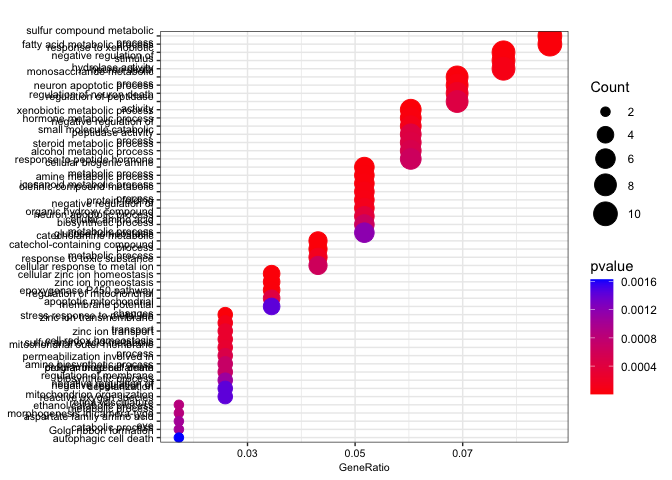
\includegraphics{figures/twas-go-hfd-1.png}

\begin{Shaded}
\begin{Highlighting}[]
\FunctionTok{barplot}\NormalTok{(go.twas.bp.enrich.simpl,}\AttributeTok{font.size=}\DecValTok{8}\NormalTok{)}
\end{Highlighting}
\end{Shaded}

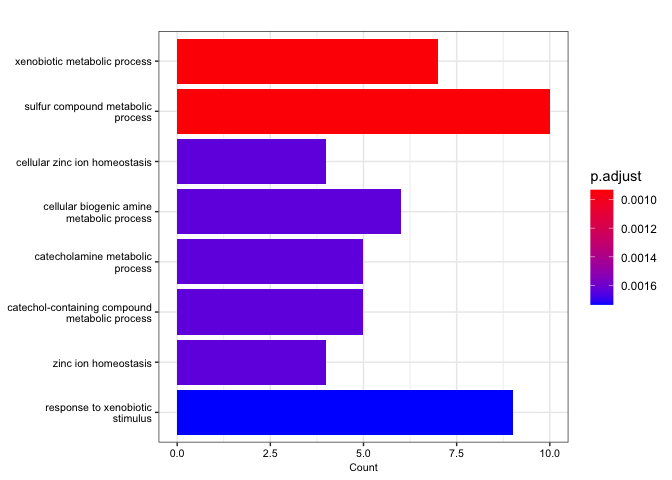
\includegraphics{figures/twas-go-hfd-2.png}

\begin{Shaded}
\begin{Highlighting}[]
\FunctionTok{cnetplot}\NormalTok{(go.twas.bp.enrich.simpl, }
         \AttributeTok{showCategory=}\DecValTok{100}\NormalTok{,}
         \AttributeTok{node\_label=}\StringTok{"gene"}\NormalTok{,}
         \AttributeTok{cex\_label\_gene=}\FloatTok{0.5}\NormalTok{)}
\end{Highlighting}
\end{Shaded}

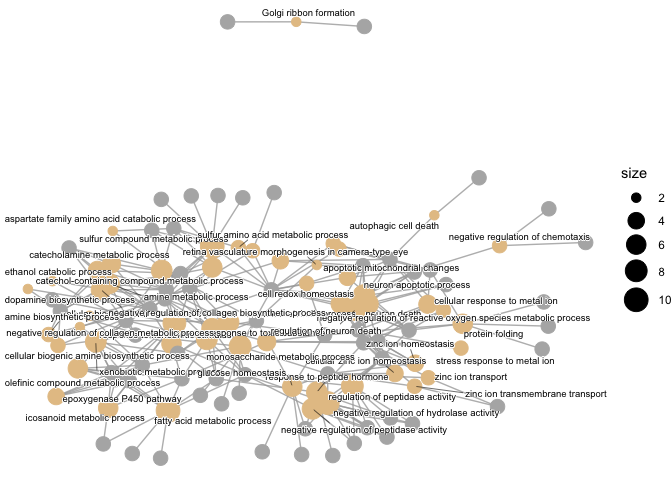
\includegraphics{figures/twas-go-hfd-3.png}

\begin{Shaded}
\begin{Highlighting}[]
\FunctionTok{cnetplot}\NormalTok{(go.twas.bp.enrich.simpl, }
         \AttributeTok{showCategory=}\DecValTok{100}\NormalTok{,}
         \AttributeTok{node\_label=}\StringTok{"category"}\NormalTok{,}
         \AttributeTok{cex\_label\_category=}\FloatTok{0.5}\NormalTok{)}
\end{Highlighting}
\end{Shaded}

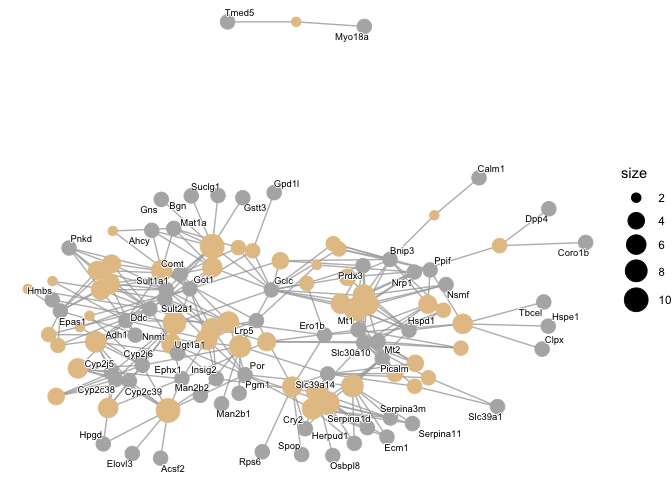
\includegraphics{figures/twas-go-hfd-4.png}

\begin{Shaded}
\begin{Highlighting}[]
\FunctionTok{heatplot}\NormalTok{(go.twas.bp.enrich.simpl)}
\end{Highlighting}
\end{Shaded}

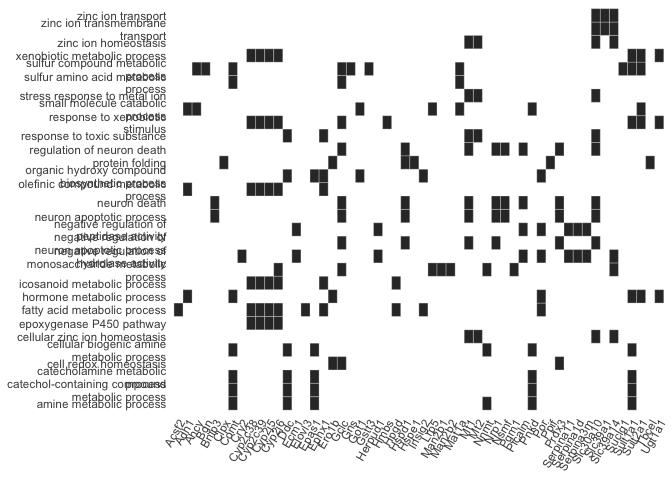
\includegraphics{figures/twas-go-hfd-5.png}

\begin{Shaded}
\begin{Highlighting}[]
\FunctionTok{library}\NormalTok{(ggupset)}
\FunctionTok{upsetplot}\NormalTok{(go.twas.bp.enrich.simpl)}
\end{Highlighting}
\end{Shaded}

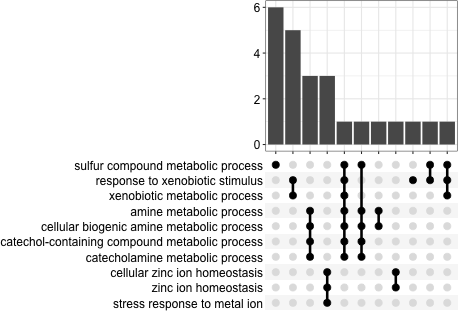
\includegraphics{figures/twas-go-hfd-6.png}

\begin{Shaded}
\begin{Highlighting}[]
\FunctionTok{dotplot}\NormalTok{(go.twas.bp.enrich.simpl, }\AttributeTok{showCategory=}\DecValTok{30}\NormalTok{)}
\end{Highlighting}
\end{Shaded}

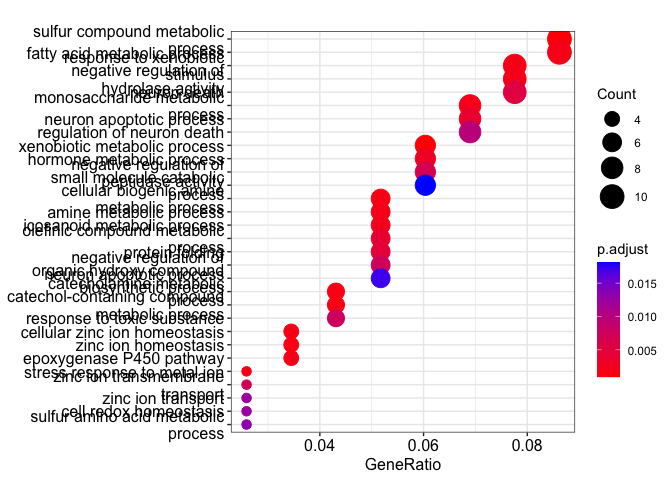
\includegraphics{figures/twas-go-hfd-7.png}

\begin{Shaded}
\begin{Highlighting}[]
\FunctionTok{heatplot}\NormalTok{(go.twas.bp.enrich.simpl, }\AttributeTok{foldChange=}\NormalTok{twas.list)}
\end{Highlighting}
\end{Shaded}

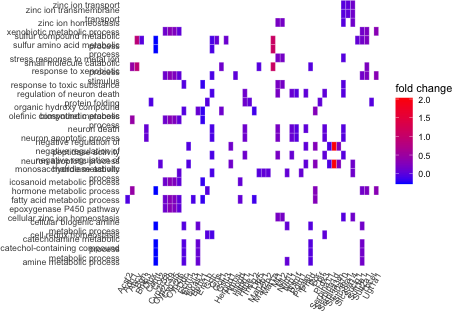
\includegraphics{figures/twas-go-hfd-8.png}

\begin{Shaded}
\begin{Highlighting}[]
\FunctionTok{upsetplot}\NormalTok{(go.twas.bp.enrich.simpl)}
\end{Highlighting}
\end{Shaded}

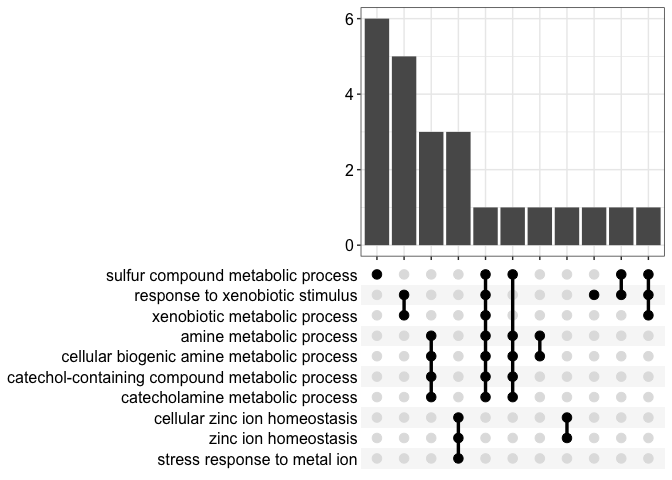
\includegraphics{figures/twas-go-hfd-9.png}

\begin{Shaded}
\begin{Highlighting}[]
\FunctionTok{as.data.frame}\NormalTok{(go.twas.bp) }\SpecialCharTok{\%\textgreater{}\%}\NormalTok{ dplyr}\SpecialCharTok{::}\FunctionTok{select}\NormalTok{(}\StringTok{"Description"}\NormalTok{,}\StringTok{"setSize"}\NormalTok{,}\StringTok{"enrichmentScore"}\NormalTok{,}\StringTok{"NES"}\NormalTok{,}\StringTok{"pvalue"}\NormalTok{,}\StringTok{"p.adjust"}\NormalTok{) }\SpecialCharTok{\%\textgreater{}\%}
  \FunctionTok{kable}\NormalTok{(}\AttributeTok{caption=}\StringTok{"HFD GO BP Analysis of TWAS Associations from GSEA"}\NormalTok{)}
\end{Highlighting}
\end{Shaded}

\begin{longtable}[]{@{}
  >{\raggedright\arraybackslash}p{(\columnwidth - 12\tabcolsep) * \real{0.1392}}
  >{\raggedright\arraybackslash}p{(\columnwidth - 12\tabcolsep) * \real{0.2911}}
  >{\raggedleft\arraybackslash}p{(\columnwidth - 12\tabcolsep) * \real{0.1013}}
  >{\raggedleft\arraybackslash}p{(\columnwidth - 12\tabcolsep) * \real{0.2025}}
  >{\raggedleft\arraybackslash}p{(\columnwidth - 12\tabcolsep) * \real{0.0633}}
  >{\raggedleft\arraybackslash}p{(\columnwidth - 12\tabcolsep) * \real{0.0886}}
  >{\raggedleft\arraybackslash}p{(\columnwidth - 12\tabcolsep) * \real{0.1139}}@{}}
\caption{HFD GO BP Analysis of TWAS Associations from
GSEA}\tabularnewline
\toprule()
\begin{minipage}[b]{\linewidth}\raggedright
\end{minipage} & \begin{minipage}[b]{\linewidth}\raggedright
Description
\end{minipage} & \begin{minipage}[b]{\linewidth}\raggedleft
setSize
\end{minipage} & \begin{minipage}[b]{\linewidth}\raggedleft
enrichmentScore
\end{minipage} & \begin{minipage}[b]{\linewidth}\raggedleft
NES
\end{minipage} & \begin{minipage}[b]{\linewidth}\raggedleft
pvalue
\end{minipage} & \begin{minipage}[b]{\linewidth}\raggedleft
p.adjust
\end{minipage} \\
\midrule()
\endfirsthead
\toprule()
\begin{minipage}[b]{\linewidth}\raggedright
\end{minipage} & \begin{minipage}[b]{\linewidth}\raggedright
Description
\end{minipage} & \begin{minipage}[b]{\linewidth}\raggedleft
setSize
\end{minipage} & \begin{minipage}[b]{\linewidth}\raggedleft
enrichmentScore
\end{minipage} & \begin{minipage}[b]{\linewidth}\raggedleft
NES
\end{minipage} & \begin{minipage}[b]{\linewidth}\raggedleft
pvalue
\end{minipage} & \begin{minipage}[b]{\linewidth}\raggedleft
p.adjust
\end{minipage} \\
\midrule()
\endhead
\url{GO:0051640} & organelle localization & 113 & 0.959 & 1.82 & 0 &
0 \\
\bottomrule()
\end{longtable}

\begin{Shaded}
\begin{Highlighting}[]
\FunctionTok{as.data.frame}\NormalTok{(go.twas.bp) }\SpecialCharTok{\%\textgreater{}\%}
  \FunctionTok{write\_csv}\NormalTok{(}\AttributeTok{file=}\StringTok{"HFD TWAS GO{-}BP GSEA.csv"}\NormalTok{)}

\FunctionTok{as.data.frame}\NormalTok{(go.twas.bp.enrich.simpl) }\SpecialCharTok{\%\textgreater{}\%}\NormalTok{ dplyr}\SpecialCharTok{::}\FunctionTok{select}\NormalTok{(}\StringTok{"Description"}\NormalTok{,}\StringTok{"GeneRatio"}\NormalTok{,}\StringTok{"Count"}\NormalTok{,}\StringTok{"pvalue"}\NormalTok{,}\StringTok{"p.adjust"}\NormalTok{) }\SpecialCharTok{\%\textgreater{}\%} 
  \FunctionTok{kable}\NormalTok{(}\AttributeTok{caption=}\StringTok{"HFD GO BP Analysis of TWAS Associations from Enrichment"}\NormalTok{)}
\end{Highlighting}
\end{Shaded}

\begin{longtable}[]{@{}
  >{\raggedright\arraybackslash}p{(\columnwidth - 10\tabcolsep) * \real{0.0894}}
  >{\raggedright\arraybackslash}p{(\columnwidth - 10\tabcolsep) * \real{0.6504}}
  >{\raggedright\arraybackslash}p{(\columnwidth - 10\tabcolsep) * \real{0.0813}}
  >{\raggedleft\arraybackslash}p{(\columnwidth - 10\tabcolsep) * \real{0.0488}}
  >{\raggedleft\arraybackslash}p{(\columnwidth - 10\tabcolsep) * \real{0.0569}}
  >{\raggedleft\arraybackslash}p{(\columnwidth - 10\tabcolsep) * \real{0.0732}}@{}}
\caption{HFD GO BP Analysis of TWAS Associations from
Enrichment}\tabularnewline
\toprule()
\begin{minipage}[b]{\linewidth}\raggedright
\end{minipage} & \begin{minipage}[b]{\linewidth}\raggedright
Description
\end{minipage} & \begin{minipage}[b]{\linewidth}\raggedright
GeneRatio
\end{minipage} & \begin{minipage}[b]{\linewidth}\raggedleft
Count
\end{minipage} & \begin{minipage}[b]{\linewidth}\raggedleft
pvalue
\end{minipage} & \begin{minipage}[b]{\linewidth}\raggedleft
p.adjust
\end{minipage} \\
\midrule()
\endfirsthead
\toprule()
\begin{minipage}[b]{\linewidth}\raggedright
\end{minipage} & \begin{minipage}[b]{\linewidth}\raggedright
Description
\end{minipage} & \begin{minipage}[b]{\linewidth}\raggedright
GeneRatio
\end{minipage} & \begin{minipage}[b]{\linewidth}\raggedleft
Count
\end{minipage} & \begin{minipage}[b]{\linewidth}\raggedleft
pvalue
\end{minipage} & \begin{minipage}[b]{\linewidth}\raggedleft
p.adjust
\end{minipage} \\
\midrule()
\endhead
\url{GO:0006805} & xenobiotic metabolic process & 7/116 & 7 & 0.000 &
0.001 \\
\url{GO:0006790} & sulfur compound metabolic process & 10/116 & 10 &
0.000 & 0.001 \\
\url{GO:0006882} & cellular zinc ion homeostasis & 4/116 & 4 & 0.000 &
0.002 \\
\url{GO:0006576} & cellular biogenic amine metabolic process & 6/116 & 6
& 0.000 & 0.002 \\
\url{GO:0006584} & catecholamine metabolic process & 5/116 & 5 & 0.000 &
0.002 \\
\url{GO:0009712} & catechol-containing compound metabolic process &
5/116 & 5 & 0.000 & 0.002 \\
\url{GO:0055069} & zinc ion homeostasis & 4/116 & 4 & 0.000 & 0.002 \\
\url{GO:0009410} & response to xenobiotic stimulus & 9/116 & 9 & 0.000 &
0.002 \\
\url{GO:0097501} & stress response to metal ion & 3/116 & 3 & 0.000 &
0.002 \\
\url{GO:0009308} & amine metabolic process & 6/116 & 6 & 0.000 &
0.002 \\
\url{GO:0019373} & epoxygenase P450 pathway & 4/116 & 4 & 0.000 &
0.002 \\
\url{GO:0006631} & fatty acid metabolic process & 10/116 & 10 & 0.000 &
0.002 \\
\url{GO:0005996} & monosaccharide metabolic process & 8/116 & 8 & 0.000
& 0.002 \\
\url{GO:0051346} & negative regulation of hydrolase activity & 9/116 & 9
& 0.000 & 0.002 \\
\url{GO:0006690} & icosanoid metabolic process & 6/116 & 6 & 0.000 &
0.002 \\
\url{GO:0042445} & hormone metabolic process & 7/116 & 7 & 0.000 &
0.003 \\
\url{GO:0051402} & neuron apoptotic process & 8/116 & 8 & 0.000 &
0.004 \\
\url{GO:0120254} & olefinic compound metabolic process & 6/116 & 6 &
0.000 & 0.004 \\
\url{GO:0006457} & protein folding & 6/116 & 6 & 0.000 & 0.005 \\
\url{GO:0070997} & neuron death & 9/116 & 9 & 0.000 & 0.005 \\
\url{GO:0010466} & negative regulation of peptidase activity & 7/116 & 7
& 0.000 & 0.007 \\
\url{GO:0071577} & zinc ion transmembrane transport & 3/116 & 3 & 0.000
& 0.007 \\
\url{GO:0043524} & negative regulation of neuron apoptotic process &
6/116 & 6 & 0.000 & 0.007 \\
\url{GO:0009636} & response to toxic substance & 5/116 & 5 & 0.000 &
0.008 \\
\url{GO:1901214} & regulation of neuron death & 8/116 & 8 & 0.000 &
0.010 \\
\url{GO:0006829} & zinc ion transport & 3/116 & 3 & 0.000 & 0.012 \\
\url{GO:0045454} & cell redox homeostasis & 3/116 & 3 & 0.000 & 0.012 \\
\url{GO:0000096} & sulfur amino acid metabolic process & 3/116 & 3 &
0.000 & 0.013 \\
\url{GO:1901617} & organic hydroxy compound biosynthetic process & 6/116
& 6 & 0.000 & 0.017 \\
\url{GO:0044282} & small molecule catabolic process & 7/116 & 7 & 0.000
& 0.018 \\
\url{GO:0051881} & regulation of mitochondrial membrane potential &
4/116 & 4 & 0.000 & 0.018 \\
\url{GO:0052547} & regulation of peptidase activity & 8/116 & 8 & 0.000
& 0.018 \\
\url{GO:0008202} & steroid metabolic process & 7/116 & 7 & 0.000 &
0.018 \\
\url{GO:1902686} & mitochondrial outer membrane permeabilization
involved in programmed cell death & 3/116 & 3 & 0.000 & 0.019 \\
\url{GO:0006066} & alcohol metabolic process & 7/116 & 7 & 0.001 &
0.020 \\
\url{GO:0071248} & cellular response to metal ion & 5/116 & 5 & 0.001 &
0.023 \\
\url{GO:0043434} & response to peptide hormone & 7/116 & 7 & 0.001 &
0.023 \\
\url{GO:0006520} & cellular amino acid metabolic process & 6/116 & 6 &
0.001 & 0.023 \\
\url{GO:0009309} & amine biosynthetic process & 3/116 & 3 & 0.001 &
0.023 \\
\url{GO:0042401} & cellular biogenic amine biosynthetic process & 3/116
& 3 & 0.001 & 0.023 \\
\url{GO:0006068} & ethanol catabolic process & 2/116 & 2 & 0.001 &
0.027 \\
\url{GO:0061299} & retina vasculature morphogenesis in camera-type eye &
2/116 & 2 & 0.001 & 0.027 \\
\url{GO:0009068} & aspartate family amino acid catabolic process & 2/116
& 2 & 0.001 & 0.031 \\
\url{GO:0090161} & Golgi ribbon formation & 2/116 & 2 & 0.001 & 0.031 \\
\url{GO:0003254} & regulation of membrane depolarization & 3/116 & 3 &
0.001 & 0.031 \\
\url{GO:0042593} & glucose homeostasis & 6/116 & 6 & 0.001 & 0.034 \\
\url{GO:0008637} & apoptotic mitochondrial changes & 4/116 & 4 & 0.001 &
0.037 \\
\url{GO:0010823} & negative regulation of mitochondrion organization &
3/116 & 3 & 0.001 & 0.037 \\
\url{GO:2000378} & negative regulation of reactive oxygen species
metabolic process & 3/116 & 3 & 0.001 & 0.037 \\
\url{GO:0048102} & autophagic cell death & 2/116 & 2 & 0.002 & 0.041 \\
\url{GO:0050922} & negative regulation of chemotaxis & 3/116 & 3 & 0.002
& 0.044 \\
\url{GO:0042416} & dopamine biosynthetic process & 2/116 & 2 & 0.002 &
0.044 \\
\url{GO:0010713} & negative regulation of collagen metabolic process &
2/116 & 2 & 0.002 & 0.048 \\
\url{GO:0032966} & negative regulation of collagen biosynthetic process
& 2/116 & 2 & 0.002 & 0.048 \\
\bottomrule()
\end{longtable}

\begin{Shaded}
\begin{Highlighting}[]
\FunctionTok{as.data.frame}\NormalTok{(go.twas.bp.enrich.simpl) }\SpecialCharTok{\%\textgreater{}\%}
  \FunctionTok{write\_csv}\NormalTok{(}\AttributeTok{file=}\StringTok{"HFD TWAS GO{-}BP Enrichment.csv"}\NormalTok{)}

\NormalTok{steroid.enrichment }\OtherTok{\textless{}{-}} \FunctionTok{as.data.frame}\NormalTok{(go.twas.bp) }\SpecialCharTok{\%\textgreater{}\%} \FunctionTok{filter}\NormalTok{(ID}\SpecialCharTok{==}\StringTok{\textquotesingle{}GO:0016126\textquotesingle{}}\NormalTok{)}
\end{Highlighting}
\end{Shaded}

\hypertarget{specific-associations}{%
\section{Specific Associations}\label{specific-associations}}

Fbp1 was one of the most highly associated results on NCD.

\begin{Shaded}
\begin{Highlighting}[]
\NormalTok{gene }\OtherTok{\textless{}{-}} \StringTok{\textquotesingle{}Fbp1\textquotesingle{}}
\NormalTok{gene.ens }\OtherTok{\textless{}{-}} \FunctionTok{filter}\NormalTok{(twas.data.ncd, symbol}\SpecialCharTok{==}\NormalTok{gene) }\SpecialCharTok{\%\textgreater{}\%} \FunctionTok{pull}\NormalTok{(ENSEMBL.ID)}
\FunctionTok{library}\NormalTok{(ggplot2)}

\NormalTok{expression.data }\SpecialCharTok{\%\textgreater{}\%}
  \FunctionTok{filter}\NormalTok{(ENSEMBL.ID }\SpecialCharTok{==}\NormalTok{ gene.ens) }\SpecialCharTok{\%\textgreater{}\%}
  \FunctionTok{pivot\_longer}\NormalTok{(}\AttributeTok{cols=}\FunctionTok{c}\NormalTok{(}\FunctionTok{starts\_with}\NormalTok{(}\StringTok{\textquotesingle{}F\textquotesingle{}}\NormalTok{),}
                      \FunctionTok{starts\_with}\NormalTok{(}\StringTok{\textquotesingle{}M\textquotesingle{}}\NormalTok{)),}
               \AttributeTok{names\_to=}\StringTok{\textquotesingle{}mouse.id\textquotesingle{}}\NormalTok{,}
               \AttributeTok{values\_to=}\StringTok{\textquotesingle{}expression\textquotesingle{}}\NormalTok{) }\SpecialCharTok{\%\textgreater{}\%}
  \FunctionTok{full\_join}\NormalTok{(phenotype.data,}\AttributeTok{by=}\StringTok{\textquotesingle{}mouse.id\textquotesingle{}}\NormalTok{) }\SpecialCharTok{\%\textgreater{}\%}
  \FunctionTok{filter}\NormalTok{(}\SpecialCharTok{!}\FunctionTok{is.na}\NormalTok{(diet)) }\SpecialCharTok{\%\textgreater{}\%}
  \FunctionTok{ggplot}\NormalTok{(}\FunctionTok{aes}\NormalTok{(}\AttributeTok{y=}\NormalTok{chol2,expression,}\AttributeTok{col=}\NormalTok{sex)) }\SpecialCharTok{+}
  \FunctionTok{geom\_point}\NormalTok{() }\SpecialCharTok{+}
  \FunctionTok{geom\_smooth}\NormalTok{(}\AttributeTok{method=}\StringTok{\textquotesingle{}lm\textquotesingle{}}\NormalTok{,}\AttributeTok{se=}\NormalTok{F) }\SpecialCharTok{+}
  \FunctionTok{facet\_grid}\NormalTok{(}\SpecialCharTok{\textasciitilde{}}\NormalTok{diet) }\SpecialCharTok{+}
  \FunctionTok{labs}\NormalTok{(}\AttributeTok{y=}\StringTok{"Cholesterol (mg/dL)"}\NormalTok{,}
       \AttributeTok{x=}\FunctionTok{paste}\NormalTok{(}\StringTok{\textquotesingle{}Expression of \textquotesingle{}}\NormalTok{, gene, }\AttributeTok{sep=}\StringTok{""}\NormalTok{))}
\end{Highlighting}
\end{Shaded}

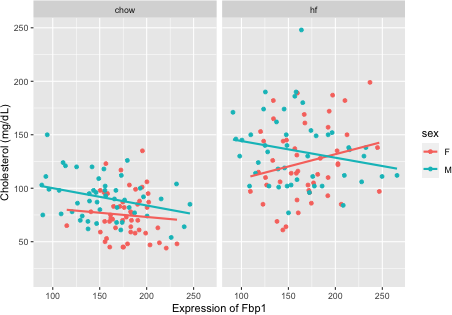
\includegraphics{figures/Fbp1-associations-1.png}

\begin{Shaded}
\begin{Highlighting}[]
\NormalTok{expression.data }\SpecialCharTok{\%\textgreater{}\%}
  \FunctionTok{filter}\NormalTok{(ENSEMBL.ID }\SpecialCharTok{==}\NormalTok{ gene.ens) }\SpecialCharTok{\%\textgreater{}\%}
  \FunctionTok{pivot\_longer}\NormalTok{(}\AttributeTok{cols=}\FunctionTok{c}\NormalTok{(}\FunctionTok{starts\_with}\NormalTok{(}\StringTok{\textquotesingle{}F\textquotesingle{}}\NormalTok{),}
                      \FunctionTok{starts\_with}\NormalTok{(}\StringTok{\textquotesingle{}M\textquotesingle{}}\NormalTok{)),}
               \AttributeTok{names\_to=}\StringTok{\textquotesingle{}mouse.id\textquotesingle{}}\NormalTok{,}
               \AttributeTok{values\_to=}\StringTok{\textquotesingle{}expression\textquotesingle{}}\NormalTok{) }\SpecialCharTok{\%\textgreater{}\%}
  \FunctionTok{full\_join}\NormalTok{(phenotype.data,}\AttributeTok{by=}\StringTok{\textquotesingle{}mouse.id\textquotesingle{}}\NormalTok{) }\SpecialCharTok{\%\textgreater{}\%}
  \FunctionTok{filter}\NormalTok{(}\SpecialCharTok{!}\FunctionTok{is.na}\NormalTok{(diet)) }\SpecialCharTok{\%\textgreater{}\%}
  \FunctionTok{filter}\NormalTok{(diet}\SpecialCharTok{==}\StringTok{\textquotesingle{}chow\textquotesingle{}}\NormalTok{) }\SpecialCharTok{\%\textgreater{}\%}
  \FunctionTok{ggplot}\NormalTok{(}\FunctionTok{aes}\NormalTok{(}\AttributeTok{y=}\NormalTok{chol2,expression,}\AttributeTok{col=}\NormalTok{sex)) }\SpecialCharTok{+}
  \FunctionTok{geom\_point}\NormalTok{() }\SpecialCharTok{+}
  \FunctionTok{geom\_smooth}\NormalTok{(}\AttributeTok{method=}\StringTok{\textquotesingle{}lm\textquotesingle{}}\NormalTok{,}\AttributeTok{se=}\NormalTok{F) }\SpecialCharTok{+}
  \FunctionTok{facet\_grid}\NormalTok{(}\SpecialCharTok{\textasciitilde{}}\NormalTok{diet) }\SpecialCharTok{+}
  \FunctionTok{labs}\NormalTok{(}\AttributeTok{y=}\StringTok{"Cholesterol (mg/dL)"}\NormalTok{,}
       \AttributeTok{x=}\FunctionTok{paste}\NormalTok{(}\StringTok{\textquotesingle{}Expression of \textquotesingle{}}\NormalTok{, gene, }\AttributeTok{sep=}\StringTok{""}\NormalTok{))}
\end{Highlighting}
\end{Shaded}

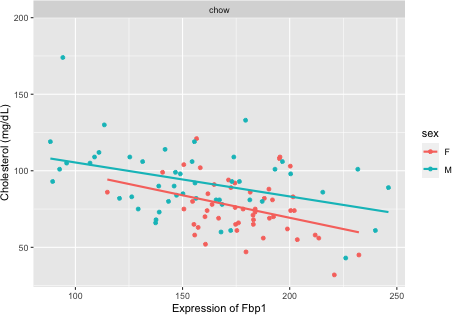
\includegraphics{figures/Fbp1-associations-2.png}

\begin{Shaded}
\begin{Highlighting}[]
\NormalTok{expression.data }\SpecialCharTok{\%\textgreater{}\%}
  \FunctionTok{filter}\NormalTok{(ENSEMBL.ID }\SpecialCharTok{==}\NormalTok{ gene.ens) }\SpecialCharTok{\%\textgreater{}\%}
  \FunctionTok{pivot\_longer}\NormalTok{(}\AttributeTok{cols=}\FunctionTok{c}\NormalTok{(}\FunctionTok{starts\_with}\NormalTok{(}\StringTok{\textquotesingle{}F\textquotesingle{}}\NormalTok{),}
                      \FunctionTok{starts\_with}\NormalTok{(}\StringTok{\textquotesingle{}M\textquotesingle{}}\NormalTok{)),}
               \AttributeTok{names\_to=}\StringTok{\textquotesingle{}mouse.id\textquotesingle{}}\NormalTok{,}
               \AttributeTok{values\_to=}\StringTok{\textquotesingle{}expression\textquotesingle{}}\NormalTok{) }\SpecialCharTok{\%\textgreater{}\%}
  \FunctionTok{full\_join}\NormalTok{(phenotype.data,}\AttributeTok{by=}\StringTok{\textquotesingle{}mouse.id\textquotesingle{}}\NormalTok{) }\SpecialCharTok{\%\textgreater{}\%}
  \FunctionTok{filter}\NormalTok{(}\SpecialCharTok{!}\FunctionTok{is.na}\NormalTok{(diet)) }\SpecialCharTok{\%\textgreater{}\%}
  \FunctionTok{filter}\NormalTok{(diet}\SpecialCharTok{==}\StringTok{\textquotesingle{}chow\textquotesingle{}}\NormalTok{) }\OtherTok{{-}\textgreater{}}\NormalTok{ fbp1.chow.data}

\FunctionTok{lm}\NormalTok{(}\AttributeTok{data=}\NormalTok{fbp1.chow.data, chol2 }\SpecialCharTok{\textasciitilde{}}\NormalTok{ expression }\SpecialCharTok{+}\NormalTok{ sex) }\SpecialCharTok{\%\textgreater{}\%}
\NormalTok{  glance}
\end{Highlighting}
\end{Shaded}

\begin{verbatim}
## # A tibble: 1 x 12
##   r.squ~1 adj.r~2 sigma stati~3 p.value    df logLik   AIC   BIC devia~4 df.re~5
##     <dbl>   <dbl> <dbl>   <dbl>   <dbl> <dbl>  <dbl> <dbl> <dbl>   <dbl>   <int>
## 1   0.176   0.159  20.6    10.2 9.96e-5     2  -434.  876.  886.  40231.      95
## # ... with 1 more variable: nobs <int>, and abbreviated variable names
## #   1: r.squared, 2: adj.r.squared, 3: statistic, 4: deviance, 5: df.residual
\end{verbatim}

\begin{Shaded}
\begin{Highlighting}[]
\NormalTok{expression.data }\SpecialCharTok{\%\textgreater{}\%}
  \FunctionTok{filter}\NormalTok{(ENSEMBL.ID }\SpecialCharTok{==}\NormalTok{ gene) }\SpecialCharTok{\%\textgreater{}\%}
  \FunctionTok{pivot\_longer}\NormalTok{(}\AttributeTok{cols=}\FunctionTok{c}\NormalTok{(}\FunctionTok{starts\_with}\NormalTok{(}\StringTok{\textquotesingle{}F\textquotesingle{}}\NormalTok{),}
                      \FunctionTok{starts\_with}\NormalTok{(}\StringTok{\textquotesingle{}M\textquotesingle{}}\NormalTok{)),}
               \AttributeTok{names\_to=}\StringTok{\textquotesingle{}mouse.id\textquotesingle{}}\NormalTok{,}
               \AttributeTok{values\_to=}\StringTok{\textquotesingle{}expression\textquotesingle{}}\NormalTok{) }\SpecialCharTok{\%\textgreater{}\%}
  \FunctionTok{full\_join}\NormalTok{(phenotype.data,}\AttributeTok{by=}\StringTok{\textquotesingle{}mouse.id\textquotesingle{}}\NormalTok{) }\SpecialCharTok{\%\textgreater{}\%}
  \FunctionTok{filter}\NormalTok{(}\SpecialCharTok{!}\FunctionTok{is.na}\NormalTok{(diet)) }\OtherTok{{-}\textgreater{}}\NormalTok{ fbp.hf.data}
\end{Highlighting}
\end{Shaded}

\hypertarget{bile-acid-metabolism}{%
\subsection{Bile Acid Metabolism}\label{bile-acid-metabolism}}

CYP7A1 is the rate limiting step for de novo \emph{bile acid}
biosynthesis

\begin{Shaded}
\begin{Highlighting}[]
\NormalTok{gene }\OtherTok{\textless{}{-}} \StringTok{\textquotesingle{}Cyp7a1\textquotesingle{}}
\NormalTok{gene.ens }\OtherTok{\textless{}{-}} \FunctionTok{filter}\NormalTok{(twas.data.ncd, symbol}\SpecialCharTok{==}\NormalTok{gene) }\SpecialCharTok{\%\textgreater{}\%} \FunctionTok{pull}\NormalTok{(ENSEMBL.ID)}

\NormalTok{expression.data }\SpecialCharTok{\%\textgreater{}\%}
  \FunctionTok{filter}\NormalTok{(ENSEMBL.ID }\SpecialCharTok{==}\NormalTok{ gene.ens) }\SpecialCharTok{\%\textgreater{}\%}
  \FunctionTok{pivot\_longer}\NormalTok{(}\AttributeTok{cols=}\FunctionTok{c}\NormalTok{(}\FunctionTok{starts\_with}\NormalTok{(}\StringTok{\textquotesingle{}F\textquotesingle{}}\NormalTok{),}
                      \FunctionTok{starts\_with}\NormalTok{(}\StringTok{\textquotesingle{}M\textquotesingle{}}\NormalTok{)),}
               \AttributeTok{names\_to=}\StringTok{\textquotesingle{}mouse.id\textquotesingle{}}\NormalTok{,}
               \AttributeTok{values\_to=}\StringTok{\textquotesingle{}expression\textquotesingle{}}\NormalTok{) }\SpecialCharTok{\%\textgreater{}\%}
  \FunctionTok{full\_join}\NormalTok{(phenotype.data,}\AttributeTok{by=}\StringTok{\textquotesingle{}mouse.id\textquotesingle{}}\NormalTok{) }\SpecialCharTok{\%\textgreater{}\%}
  \FunctionTok{filter}\NormalTok{(}\SpecialCharTok{!}\FunctionTok{is.na}\NormalTok{(diet)) }\SpecialCharTok{\%\textgreater{}\%}
  \FunctionTok{ggplot}\NormalTok{(}\FunctionTok{aes}\NormalTok{(}\AttributeTok{y=}\NormalTok{chol2,expression,}\AttributeTok{col=}\NormalTok{sex)) }\SpecialCharTok{+}
  \FunctionTok{geom\_point}\NormalTok{() }\SpecialCharTok{+}
  \FunctionTok{geom\_smooth}\NormalTok{(}\AttributeTok{method=}\StringTok{\textquotesingle{}lm\textquotesingle{}}\NormalTok{,}\AttributeTok{se=}\NormalTok{F) }\SpecialCharTok{+}
  \FunctionTok{facet\_grid}\NormalTok{(}\SpecialCharTok{\textasciitilde{}}\NormalTok{diet) }\SpecialCharTok{+}
  \FunctionTok{labs}\NormalTok{(}\AttributeTok{y=}\StringTok{"Cholesterol (mg/dL)"}\NormalTok{,}
       \AttributeTok{x=}\FunctionTok{paste}\NormalTok{(}\StringTok{\textquotesingle{}Expression of \textquotesingle{}}\NormalTok{, gene, }\AttributeTok{sep=}\StringTok{""}\NormalTok{))}
\end{Highlighting}
\end{Shaded}

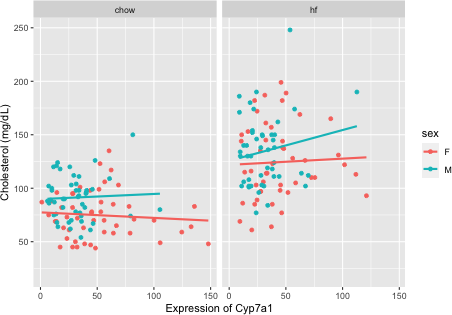
\includegraphics{figures/cyp7a1-associations-1.png}

\begin{Shaded}
\begin{Highlighting}[]
\NormalTok{expression.data }\SpecialCharTok{\%\textgreater{}\%}
  \FunctionTok{filter}\NormalTok{(ENSEMBL.ID }\SpecialCharTok{==}\NormalTok{ gene.ens) }\SpecialCharTok{\%\textgreater{}\%}
  \FunctionTok{pivot\_longer}\NormalTok{(}\AttributeTok{cols=}\FunctionTok{c}\NormalTok{(}\FunctionTok{starts\_with}\NormalTok{(}\StringTok{\textquotesingle{}F\textquotesingle{}}\NormalTok{),}
                      \FunctionTok{starts\_with}\NormalTok{(}\StringTok{\textquotesingle{}M\textquotesingle{}}\NormalTok{)),}
               \AttributeTok{names\_to=}\StringTok{\textquotesingle{}mouse.id\textquotesingle{}}\NormalTok{,}
               \AttributeTok{values\_to=}\StringTok{\textquotesingle{}expression\textquotesingle{}}\NormalTok{) }\SpecialCharTok{\%\textgreater{}\%}
  \FunctionTok{full\_join}\NormalTok{(phenotype.data,}\AttributeTok{by=}\StringTok{\textquotesingle{}mouse.id\textquotesingle{}}\NormalTok{) }\SpecialCharTok{\%\textgreater{}\%}
  \FunctionTok{filter}\NormalTok{(}\SpecialCharTok{!}\FunctionTok{is.na}\NormalTok{(diet)) }\SpecialCharTok{\%\textgreater{}\%}
  \FunctionTok{filter}\NormalTok{(diet}\SpecialCharTok{==}\StringTok{\textquotesingle{}chow\textquotesingle{}}\NormalTok{) }\OtherTok{{-}\textgreater{}}\NormalTok{ gene.chow.data}

\FunctionTok{lm}\NormalTok{(}\AttributeTok{data=}\NormalTok{gene.chow.data, chol2 }\SpecialCharTok{\textasciitilde{}}\NormalTok{ expression }\SpecialCharTok{+}\NormalTok{ sex) }\SpecialCharTok{\%\textgreater{}\%}
\NormalTok{  tidy }\SpecialCharTok{\%\textgreater{}\%}
  \FunctionTok{kable}\NormalTok{(}\AttributeTok{caption=}\StringTok{"Summary associations of Cyp7a1 and cholesterol on chow"}\NormalTok{)}
\end{Highlighting}
\end{Shaded}

\begin{longtable}[]{@{}lrrrr@{}}
\caption{Summary associations of Cyp7a1 and cholesterol on
chow}\tabularnewline
\toprule()
term & estimate & std.error & statistic & p.value \\
\midrule()
\endfirsthead
\toprule()
term & estimate & std.error & statistic & p.value \\
\midrule()
\endhead
(Intercept) & 76.191 & 4.881 & 15.611 & 0.000 \\
expression & -0.027 & 0.076 & -0.355 & 0.724 \\
sexM & 15.954 & 4.518 & 3.531 & 0.001 \\
\bottomrule()
\end{longtable}

\begin{Shaded}
\begin{Highlighting}[]
\NormalTok{expression.data }\SpecialCharTok{\%\textgreater{}\%}
  \FunctionTok{filter}\NormalTok{(ENSEMBL.ID }\SpecialCharTok{==}\NormalTok{ gene.ens) }\SpecialCharTok{\%\textgreater{}\%}
  \FunctionTok{pivot\_longer}\NormalTok{(}\AttributeTok{cols=}\FunctionTok{c}\NormalTok{(}\FunctionTok{starts\_with}\NormalTok{(}\StringTok{\textquotesingle{}F\textquotesingle{}}\NormalTok{),}
                      \FunctionTok{starts\_with}\NormalTok{(}\StringTok{\textquotesingle{}M\textquotesingle{}}\NormalTok{)),}
               \AttributeTok{names\_to=}\StringTok{\textquotesingle{}mouse.id\textquotesingle{}}\NormalTok{,}
               \AttributeTok{values\_to=}\StringTok{\textquotesingle{}expression\textquotesingle{}}\NormalTok{) }\SpecialCharTok{\%\textgreater{}\%}
  \FunctionTok{full\_join}\NormalTok{(phenotype.data,}\AttributeTok{by=}\StringTok{\textquotesingle{}mouse.id\textquotesingle{}}\NormalTok{) }\SpecialCharTok{\%\textgreater{}\%}
  \FunctionTok{filter}\NormalTok{(}\SpecialCharTok{!}\FunctionTok{is.na}\NormalTok{(diet)) }\OtherTok{{-}\textgreater{}}\NormalTok{ gene.hf.data}

\FunctionTok{lm}\NormalTok{(}\AttributeTok{data=}\NormalTok{gene.hf.data, chol2 }\SpecialCharTok{\textasciitilde{}}\NormalTok{ expression }\SpecialCharTok{+}\NormalTok{ sex) }\SpecialCharTok{\%\textgreater{}\%}
\NormalTok{  tidy }\SpecialCharTok{\%\textgreater{}\%}
  \FunctionTok{kable}\NormalTok{(}\AttributeTok{caption=}\StringTok{"Summary associations of Cyp7a1 and cholesterol on HFD"}\NormalTok{)}
\end{Highlighting}
\end{Shaded}

\begin{longtable}[]{@{}lrrrr@{}}
\caption{Summary associations of Cyp7a1 and cholesterol on
HFD}\tabularnewline
\toprule()
term & estimate & std.error & statistic & p.value \\
\midrule()
\endfirsthead
\toprule()
term & estimate & std.error & statistic & p.value \\
\midrule()
\endhead
(Intercept) & 100.060 & 6.108 & 16.381 & 0.000 \\
expression & -0.026 & 0.103 & -0.255 & 0.799 \\
sexM & 13.262 & 5.565 & 2.383 & 0.018 \\
\bottomrule()
\end{longtable}

\hypertarget{scd1}{%
\subsection{SCD1}\label{scd1}}

SCD1 is the gene with the biggest effect size on NCD

\begin{Shaded}
\begin{Highlighting}[]
\NormalTok{gene }\OtherTok{\textless{}{-}} \StringTok{\textquotesingle{}Scd1\textquotesingle{}}
\NormalTok{gene.ens }\OtherTok{\textless{}{-}} \FunctionTok{filter}\NormalTok{(twas.data.ncd, symbol}\SpecialCharTok{==}\NormalTok{gene) }\SpecialCharTok{\%\textgreater{}\%} \FunctionTok{pull}\NormalTok{(ENSEMBL.ID)}

\NormalTok{expression.data }\SpecialCharTok{\%\textgreater{}\%}
  \FunctionTok{filter}\NormalTok{(ENSEMBL.ID }\SpecialCharTok{==}\NormalTok{ gene.ens) }\SpecialCharTok{\%\textgreater{}\%}
  \FunctionTok{pivot\_longer}\NormalTok{(}\AttributeTok{cols=}\FunctionTok{c}\NormalTok{(}\FunctionTok{starts\_with}\NormalTok{(}\StringTok{\textquotesingle{}F\textquotesingle{}}\NormalTok{),}
                      \FunctionTok{starts\_with}\NormalTok{(}\StringTok{\textquotesingle{}M\textquotesingle{}}\NormalTok{)),}
               \AttributeTok{names\_to=}\StringTok{\textquotesingle{}mouse.id\textquotesingle{}}\NormalTok{,}
               \AttributeTok{values\_to=}\StringTok{\textquotesingle{}expression\textquotesingle{}}\NormalTok{) }\SpecialCharTok{\%\textgreater{}\%}
  \FunctionTok{full\_join}\NormalTok{(phenotype.data,}\AttributeTok{by=}\StringTok{\textquotesingle{}mouse.id\textquotesingle{}}\NormalTok{) }\SpecialCharTok{\%\textgreater{}\%}
  \FunctionTok{filter}\NormalTok{(}\SpecialCharTok{!}\FunctionTok{is.na}\NormalTok{(diet)) }\SpecialCharTok{\%\textgreater{}\%}
  \FunctionTok{ggplot}\NormalTok{(}\FunctionTok{aes}\NormalTok{(}\AttributeTok{y=}\NormalTok{chol2,expression,}\AttributeTok{col=}\NormalTok{sex)) }\SpecialCharTok{+}
  \FunctionTok{geom\_point}\NormalTok{() }\SpecialCharTok{+}
  \FunctionTok{geom\_smooth}\NormalTok{(}\AttributeTok{method=}\StringTok{\textquotesingle{}lm\textquotesingle{}}\NormalTok{,}\AttributeTok{se=}\NormalTok{F) }\SpecialCharTok{+}
  \FunctionTok{facet\_grid}\NormalTok{(}\SpecialCharTok{\textasciitilde{}}\NormalTok{diet) }\SpecialCharTok{+}
  \FunctionTok{labs}\NormalTok{(}\AttributeTok{y=}\StringTok{"Cholesterol (mg/dL)"}\NormalTok{,}
       \AttributeTok{x=}\FunctionTok{paste}\NormalTok{(}\StringTok{\textquotesingle{}Expression of \textquotesingle{}}\NormalTok{, gene, }\AttributeTok{sep=}\StringTok{""}\NormalTok{))}
\end{Highlighting}
\end{Shaded}

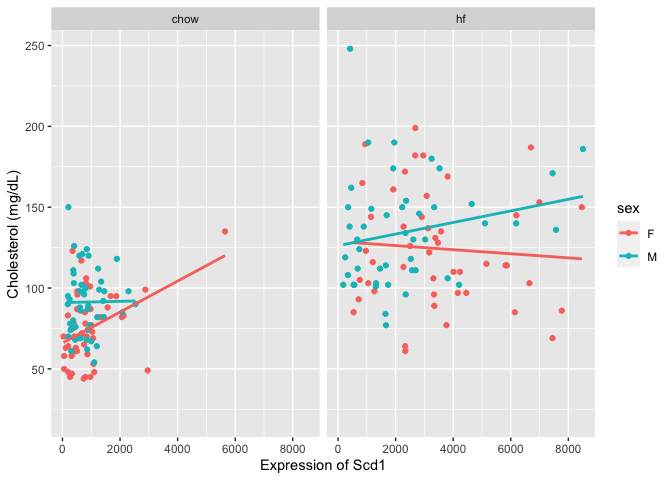
\includegraphics{figures/scd1-associations-1.png}

\begin{Shaded}
\begin{Highlighting}[]
\NormalTok{expression.data }\SpecialCharTok{\%\textgreater{}\%}
  \FunctionTok{filter}\NormalTok{(ENSEMBL.ID }\SpecialCharTok{==}\NormalTok{ gene.ens) }\SpecialCharTok{\%\textgreater{}\%}
  \FunctionTok{pivot\_longer}\NormalTok{(}\AttributeTok{cols=}\FunctionTok{c}\NormalTok{(}\FunctionTok{starts\_with}\NormalTok{(}\StringTok{\textquotesingle{}F\textquotesingle{}}\NormalTok{),}
                      \FunctionTok{starts\_with}\NormalTok{(}\StringTok{\textquotesingle{}M\textquotesingle{}}\NormalTok{)),}
               \AttributeTok{names\_to=}\StringTok{\textquotesingle{}mouse.id\textquotesingle{}}\NormalTok{,}
               \AttributeTok{values\_to=}\StringTok{\textquotesingle{}expression\textquotesingle{}}\NormalTok{) }\SpecialCharTok{\%\textgreater{}\%}
  \FunctionTok{full\_join}\NormalTok{(phenotype.data,}\AttributeTok{by=}\StringTok{\textquotesingle{}mouse.id\textquotesingle{}}\NormalTok{) }\SpecialCharTok{\%\textgreater{}\%}
  \FunctionTok{filter}\NormalTok{(}\SpecialCharTok{!}\FunctionTok{is.na}\NormalTok{(diet)) }\SpecialCharTok{\%\textgreater{}\%}
  \FunctionTok{filter}\NormalTok{(diet}\SpecialCharTok{==}\StringTok{\textquotesingle{}chow\textquotesingle{}}\NormalTok{) }\OtherTok{{-}\textgreater{}}\NormalTok{ gene.chow.data}

\FunctionTok{lm}\NormalTok{(}\AttributeTok{data=}\NormalTok{gene.chow.data, chol2 }\SpecialCharTok{\textasciitilde{}}\NormalTok{ expression }\SpecialCharTok{+}\NormalTok{ sex) }\SpecialCharTok{\%\textgreater{}\%}
\NormalTok{  tidy }\SpecialCharTok{\%\textgreater{}\%}
  \FunctionTok{kable}\NormalTok{(}\AttributeTok{caption=}\StringTok{"Summary associations of Scd1 and cholesterol on chow"}\NormalTok{)}
\end{Highlighting}
\end{Shaded}

\begin{longtable}[]{@{}lrrrr@{}}
\caption{Summary associations of Scd1 and cholesterol on
chow}\tabularnewline
\toprule()
term & estimate & std.error & statistic & p.value \\
\midrule()
\endfirsthead
\toprule()
term & estimate & std.error & statistic & p.value \\
\midrule()
\endhead
(Intercept) & 68.093 & 3.775 & 18.04 & 0.000 \\
expression & 0.007 & 0.003 & 2.74 & 0.007 \\
sexM & 17.118 & 4.105 & 4.17 & 0.000 \\
\bottomrule()
\end{longtable}

\begin{Shaded}
\begin{Highlighting}[]
\FunctionTok{library}\NormalTok{(MASS)}
\FunctionTok{rlm}\NormalTok{(}\AttributeTok{data=}\NormalTok{gene.chow.data, chol2 }\SpecialCharTok{\textasciitilde{}}\NormalTok{ expression }\SpecialCharTok{+}\NormalTok{ sex) }\SpecialCharTok{\%\textgreater{}\%}
\NormalTok{  tidy }\SpecialCharTok{\%\textgreater{}\%}
  \FunctionTok{kable}\NormalTok{(}\AttributeTok{caption=}\StringTok{"Summary associations of Scd1 and cholesterol on chow, using robust linear models"}\NormalTok{)}
\end{Highlighting}
\end{Shaded}

\begin{longtable}[]{@{}lrrr@{}}
\caption{Summary associations of Scd1 and cholesterol on chow, using
robust linear models}\tabularnewline
\toprule()
term & estimate & std.error & statistic \\
\midrule()
\endfirsthead
\toprule()
term & estimate & std.error & statistic \\
\midrule()
\endhead
(Intercept) & 65.735 & 3.908 & 16.82 \\
expression & 0.009 & 0.003 & 3.30 \\
sexM & 16.623 & 4.250 & 3.91 \\
\bottomrule()
\end{longtable}

\begin{Shaded}
\begin{Highlighting}[]
\NormalTok{expression.data }\SpecialCharTok{\%\textgreater{}\%}
  \FunctionTok{filter}\NormalTok{(ENSEMBL.ID }\SpecialCharTok{==}\NormalTok{ gene.ens) }\SpecialCharTok{\%\textgreater{}\%}
  \FunctionTok{pivot\_longer}\NormalTok{(}\AttributeTok{cols=}\FunctionTok{c}\NormalTok{(}\FunctionTok{starts\_with}\NormalTok{(}\StringTok{\textquotesingle{}F\textquotesingle{}}\NormalTok{),}
                      \FunctionTok{starts\_with}\NormalTok{(}\StringTok{\textquotesingle{}M\textquotesingle{}}\NormalTok{)),}
               \AttributeTok{names\_to=}\StringTok{\textquotesingle{}mouse.id\textquotesingle{}}\NormalTok{,}
               \AttributeTok{values\_to=}\StringTok{\textquotesingle{}expression\textquotesingle{}}\NormalTok{) }\SpecialCharTok{\%\textgreater{}\%}
  \FunctionTok{full\_join}\NormalTok{(phenotype.data,}\AttributeTok{by=}\StringTok{\textquotesingle{}mouse.id\textquotesingle{}}\NormalTok{) }\SpecialCharTok{\%\textgreater{}\%}
  \FunctionTok{filter}\NormalTok{(}\SpecialCharTok{!}\FunctionTok{is.na}\NormalTok{(diet)) }\OtherTok{{-}\textgreater{}}\NormalTok{ gene.hf.data}

\FunctionTok{lm}\NormalTok{(}\AttributeTok{data=}\NormalTok{gene.hf.data, chol2 }\SpecialCharTok{\textasciitilde{}}\NormalTok{ expression }\SpecialCharTok{+}\NormalTok{ sex) }\SpecialCharTok{\%\textgreater{}\%}
\NormalTok{  tidy }\SpecialCharTok{\%\textgreater{}\%}
  \FunctionTok{kable}\NormalTok{(}\AttributeTok{caption=}\StringTok{"Summary associations of Scd1 and cholesterol on HFD"}\NormalTok{)}
\end{Highlighting}
\end{Shaded}

\begin{longtable}[]{@{}lrrrr@{}}
\caption{Summary associations of Scd1 and cholesterol on
HFD}\tabularnewline
\toprule()
term & estimate & std.error & statistic & p.value \\
\midrule()
\endfirsthead
\toprule()
term & estimate & std.error & statistic & p.value \\
\midrule()
\endhead
(Intercept) & 80.778 & 4.398 & 18.37 & 0 \\
expression & 0.008 & 0.001 & 6.40 & 0 \\
sexM & 18.589 & 4.874 & 3.81 & 0 \\
\bottomrule()
\end{longtable}

\hypertarget{serpina3k}{%
\subsection{Serpina3k}\label{serpina3k}}

Serpina3k is the gene with the biggest inverse effect size on NCD

\begin{Shaded}
\begin{Highlighting}[]
\NormalTok{gene }\OtherTok{\textless{}{-}} \StringTok{\textquotesingle{}Serpina3k\textquotesingle{}}
\NormalTok{gene.ens }\OtherTok{\textless{}{-}} \FunctionTok{filter}\NormalTok{(twas.data.ncd, symbol}\SpecialCharTok{==}\NormalTok{gene) }\SpecialCharTok{\%\textgreater{}\%} \FunctionTok{pull}\NormalTok{(ENSEMBL.ID)}

\NormalTok{expression.data }\SpecialCharTok{\%\textgreater{}\%}
  \FunctionTok{filter}\NormalTok{(ENSEMBL.ID }\SpecialCharTok{==}\NormalTok{ gene.ens) }\SpecialCharTok{\%\textgreater{}\%}
  \FunctionTok{pivot\_longer}\NormalTok{(}\AttributeTok{cols=}\FunctionTok{c}\NormalTok{(}\FunctionTok{starts\_with}\NormalTok{(}\StringTok{\textquotesingle{}F\textquotesingle{}}\NormalTok{),}
                      \FunctionTok{starts\_with}\NormalTok{(}\StringTok{\textquotesingle{}M\textquotesingle{}}\NormalTok{)),}
               \AttributeTok{names\_to=}\StringTok{\textquotesingle{}mouse.id\textquotesingle{}}\NormalTok{,}
               \AttributeTok{values\_to=}\StringTok{\textquotesingle{}expression\textquotesingle{}}\NormalTok{) }\SpecialCharTok{\%\textgreater{}\%}
  \FunctionTok{full\_join}\NormalTok{(phenotype.data,}\AttributeTok{by=}\StringTok{\textquotesingle{}mouse.id\textquotesingle{}}\NormalTok{) }\SpecialCharTok{\%\textgreater{}\%}
  \FunctionTok{filter}\NormalTok{(}\SpecialCharTok{!}\FunctionTok{is.na}\NormalTok{(diet)) }\SpecialCharTok{\%\textgreater{}\%}
  \FunctionTok{ggplot}\NormalTok{(}\FunctionTok{aes}\NormalTok{(}\AttributeTok{y=}\NormalTok{chol2,expression,}\AttributeTok{col=}\NormalTok{sex)) }\SpecialCharTok{+}
  \FunctionTok{geom\_point}\NormalTok{() }\SpecialCharTok{+}
  \FunctionTok{geom\_smooth}\NormalTok{(}\AttributeTok{method=}\StringTok{\textquotesingle{}lm\textquotesingle{}}\NormalTok{,}\AttributeTok{se=}\NormalTok{F) }\SpecialCharTok{+}
  \FunctionTok{facet\_grid}\NormalTok{(}\SpecialCharTok{\textasciitilde{}}\NormalTok{diet) }\SpecialCharTok{+}
  \FunctionTok{labs}\NormalTok{(}\AttributeTok{y=}\StringTok{"Cholesterol (mg/dL)"}\NormalTok{,}
       \AttributeTok{x=}\FunctionTok{paste}\NormalTok{(}\StringTok{\textquotesingle{}Expression of \textquotesingle{}}\NormalTok{, gene, }\AttributeTok{sep=}\StringTok{""}\NormalTok{))}
\end{Highlighting}
\end{Shaded}

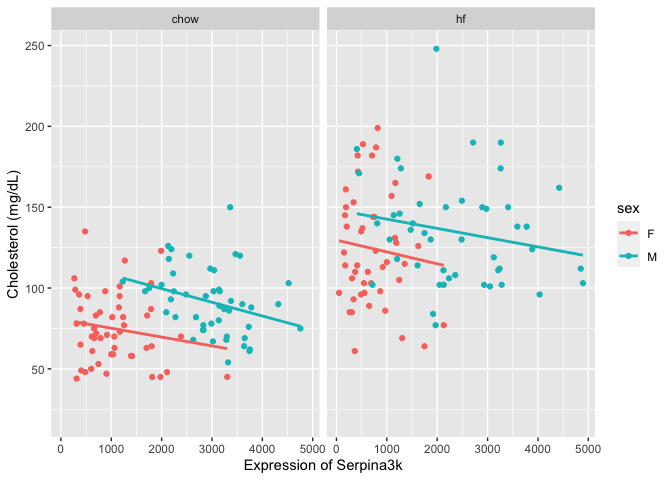
\includegraphics{figures/serpina3k-associations-1.png}

\begin{Shaded}
\begin{Highlighting}[]
\NormalTok{expression.data }\SpecialCharTok{\%\textgreater{}\%}
  \FunctionTok{filter}\NormalTok{(ENSEMBL.ID }\SpecialCharTok{==}\NormalTok{ gene.ens) }\SpecialCharTok{\%\textgreater{}\%}
  \FunctionTok{pivot\_longer}\NormalTok{(}\AttributeTok{cols=}\FunctionTok{c}\NormalTok{(}\FunctionTok{starts\_with}\NormalTok{(}\StringTok{\textquotesingle{}F\textquotesingle{}}\NormalTok{),}
                      \FunctionTok{starts\_with}\NormalTok{(}\StringTok{\textquotesingle{}M\textquotesingle{}}\NormalTok{)),}
               \AttributeTok{names\_to=}\StringTok{\textquotesingle{}mouse.id\textquotesingle{}}\NormalTok{,}
               \AttributeTok{values\_to=}\StringTok{\textquotesingle{}expression\textquotesingle{}}\NormalTok{) }\SpecialCharTok{\%\textgreater{}\%}
  \FunctionTok{full\_join}\NormalTok{(phenotype.data,}\AttributeTok{by=}\StringTok{\textquotesingle{}mouse.id\textquotesingle{}}\NormalTok{) }\SpecialCharTok{\%\textgreater{}\%}
  \FunctionTok{filter}\NormalTok{(}\SpecialCharTok{!}\FunctionTok{is.na}\NormalTok{(diet)) }\SpecialCharTok{\%\textgreater{}\%}
  \FunctionTok{filter}\NormalTok{(diet}\SpecialCharTok{==}\StringTok{\textquotesingle{}chow\textquotesingle{}}\NormalTok{) }\OtherTok{{-}\textgreater{}}\NormalTok{ gene.chow.data}

\FunctionTok{lm}\NormalTok{(}\AttributeTok{data=}\NormalTok{gene.chow.data, chol2 }\SpecialCharTok{\textasciitilde{}}\NormalTok{ expression }\SpecialCharTok{+}\NormalTok{ sex) }\SpecialCharTok{\%\textgreater{}\%}
\NormalTok{  tidy }\SpecialCharTok{\%\textgreater{}\%}
  \FunctionTok{kable}\NormalTok{(}\AttributeTok{caption=}\StringTok{"Summary associations of Serpina3k and cholesterol on chow"}\NormalTok{)}
\end{Highlighting}
\end{Shaded}

\begin{longtable}[]{@{}lrrrr@{}}
\caption{Summary associations of Serpina3k and cholesterol on
chow}\tabularnewline
\toprule()
term & estimate & std.error & statistic & p.value \\
\midrule()
\endfirsthead
\toprule()
term & estimate & std.error & statistic & p.value \\
\midrule()
\endhead
(Intercept) & 82.390 & 4.331 & 19.02 & 0.000 \\
expression & -0.007 & 0.003 & -2.35 & 0.021 \\
sexM & 30.226 & 7.160 & 4.22 & 0.000 \\
\bottomrule()
\end{longtable}

\begin{Shaded}
\begin{Highlighting}[]
\FunctionTok{library}\NormalTok{(MASS)}
\FunctionTok{rlm}\NormalTok{(}\AttributeTok{data=}\NormalTok{gene.chow.data, chol2 }\SpecialCharTok{\textasciitilde{}}\NormalTok{ expression }\SpecialCharTok{+}\NormalTok{ sex) }\SpecialCharTok{\%\textgreater{}\%}
\NormalTok{  tidy }\SpecialCharTok{\%\textgreater{}\%}
  \FunctionTok{kable}\NormalTok{(}\AttributeTok{caption=}\StringTok{"Summary associations of Serpina3k and cholesterol on chow, using robust linear models"}\NormalTok{)}
\end{Highlighting}
\end{Shaded}

\begin{longtable}[]{@{}lrrr@{}}
\caption{Summary associations of Serpina3k and cholesterol on chow,
using robust linear models}\tabularnewline
\toprule()
term & estimate & std.error & statistic \\
\midrule()
\endfirsthead
\toprule()
term & estimate & std.error & statistic \\
\midrule()
\endhead
(Intercept) & 81.991 & 4.226 & 19.40 \\
expression & -0.008 & 0.003 & -2.74 \\
sexM & 32.690 & 6.985 & 4.68 \\
\bottomrule()
\end{longtable}

\begin{Shaded}
\begin{Highlighting}[]
\NormalTok{expression.data }\SpecialCharTok{\%\textgreater{}\%}
  \FunctionTok{filter}\NormalTok{(ENSEMBL.ID }\SpecialCharTok{==}\NormalTok{ gene.ens) }\SpecialCharTok{\%\textgreater{}\%}
  \FunctionTok{pivot\_longer}\NormalTok{(}\AttributeTok{cols=}\FunctionTok{c}\NormalTok{(}\FunctionTok{starts\_with}\NormalTok{(}\StringTok{\textquotesingle{}F\textquotesingle{}}\NormalTok{),}
                      \FunctionTok{starts\_with}\NormalTok{(}\StringTok{\textquotesingle{}M\textquotesingle{}}\NormalTok{)),}
               \AttributeTok{names\_to=}\StringTok{\textquotesingle{}mouse.id\textquotesingle{}}\NormalTok{,}
               \AttributeTok{values\_to=}\StringTok{\textquotesingle{}expression\textquotesingle{}}\NormalTok{) }\SpecialCharTok{\%\textgreater{}\%}
  \FunctionTok{full\_join}\NormalTok{(phenotype.data,}\AttributeTok{by=}\StringTok{\textquotesingle{}mouse.id\textquotesingle{}}\NormalTok{) }\SpecialCharTok{\%\textgreater{}\%}
  \FunctionTok{filter}\NormalTok{(}\SpecialCharTok{!}\FunctionTok{is.na}\NormalTok{(diet)) }\OtherTok{{-}\textgreater{}}\NormalTok{ gene.hf.data}

\FunctionTok{lm}\NormalTok{(}\AttributeTok{data=}\NormalTok{gene.hf.data, chol2 }\SpecialCharTok{\textasciitilde{}}\NormalTok{ expression }\SpecialCharTok{+}\NormalTok{ sex) }\SpecialCharTok{\%\textgreater{}\%}
\NormalTok{  tidy }\SpecialCharTok{\%\textgreater{}\%}
  \FunctionTok{kable}\NormalTok{(}\AttributeTok{caption=}\StringTok{"Summary associations of Serpina3k and cholesterol on HFD"}\NormalTok{)}
\end{Highlighting}
\end{Shaded}

\begin{longtable}[]{@{}lrrrr@{}}
\caption{Summary associations of Serpina3k and cholesterol on
HFD}\tabularnewline
\toprule()
term & estimate & std.error & statistic & p.value \\
\midrule()
\endfirsthead
\toprule()
term & estimate & std.error & statistic & p.value \\
\midrule()
\endhead
(Intercept) & 111.314 & 4.516 & 24.65 & 0 \\
expression & -0.014 & 0.003 & -4.46 & 0 \\
sexM & 38.748 & 7.554 & 5.13 & 0 \\
\bottomrule()
\end{longtable}

\hypertarget{ugt1a5}{%
\subsection{Ugt1a5}\label{ugt1a5}}

Ugt1a5 is the gene with the most significant effect on ncd

\begin{Shaded}
\begin{Highlighting}[]
\NormalTok{gene }\OtherTok{\textless{}{-}} \StringTok{\textquotesingle{}Ugt1a5\textquotesingle{}}
\NormalTok{gene.ens }\OtherTok{\textless{}{-}} \FunctionTok{filter}\NormalTok{(twas.data.ncd, symbol}\SpecialCharTok{==}\NormalTok{gene) }\SpecialCharTok{\%\textgreater{}\%} \FunctionTok{pull}\NormalTok{(ENSEMBL.ID)}

\NormalTok{expression.data }\SpecialCharTok{\%\textgreater{}\%}
  \FunctionTok{filter}\NormalTok{(ENSEMBL.ID }\SpecialCharTok{==}\NormalTok{ gene.ens) }\SpecialCharTok{\%\textgreater{}\%}
  \FunctionTok{pivot\_longer}\NormalTok{(}\AttributeTok{cols=}\FunctionTok{c}\NormalTok{(}\FunctionTok{starts\_with}\NormalTok{(}\StringTok{\textquotesingle{}F\textquotesingle{}}\NormalTok{),}
                      \FunctionTok{starts\_with}\NormalTok{(}\StringTok{\textquotesingle{}M\textquotesingle{}}\NormalTok{)),}
               \AttributeTok{names\_to=}\StringTok{\textquotesingle{}mouse.id\textquotesingle{}}\NormalTok{,}
               \AttributeTok{values\_to=}\StringTok{\textquotesingle{}expression\textquotesingle{}}\NormalTok{) }\SpecialCharTok{\%\textgreater{}\%}
  \FunctionTok{full\_join}\NormalTok{(phenotype.data,}\AttributeTok{by=}\StringTok{\textquotesingle{}mouse.id\textquotesingle{}}\NormalTok{) }\SpecialCharTok{\%\textgreater{}\%}
  \FunctionTok{filter}\NormalTok{(}\SpecialCharTok{!}\FunctionTok{is.na}\NormalTok{(diet)) }\SpecialCharTok{\%\textgreater{}\%}
  \FunctionTok{ggplot}\NormalTok{(}\FunctionTok{aes}\NormalTok{(}\AttributeTok{y=}\NormalTok{chol2,expression,}\AttributeTok{col=}\NormalTok{sex)) }\SpecialCharTok{+}
  \FunctionTok{geom\_point}\NormalTok{() }\SpecialCharTok{+}
  \FunctionTok{geom\_smooth}\NormalTok{(}\AttributeTok{method=}\StringTok{\textquotesingle{}lm\textquotesingle{}}\NormalTok{,}\AttributeTok{se=}\NormalTok{F) }\SpecialCharTok{+}
  \FunctionTok{facet\_grid}\NormalTok{(}\SpecialCharTok{\textasciitilde{}}\NormalTok{diet) }\SpecialCharTok{+}
  \FunctionTok{labs}\NormalTok{(}\AttributeTok{y=}\StringTok{"Cholesterol (mg/dL)"}\NormalTok{,}
       \AttributeTok{x=}\FunctionTok{paste}\NormalTok{(}\StringTok{\textquotesingle{}Expression of \textquotesingle{}}\NormalTok{, gene, }\AttributeTok{sep=}\StringTok{""}\NormalTok{))}
\end{Highlighting}
\end{Shaded}

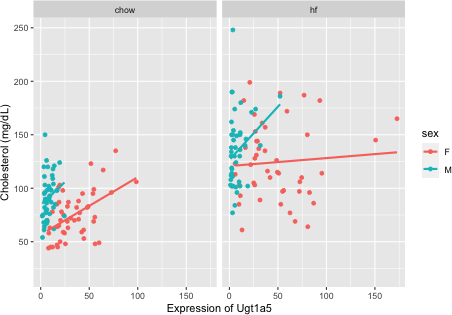
\includegraphics{figures/Ugt1a5-associations-1.png}

\begin{Shaded}
\begin{Highlighting}[]
\NormalTok{expression.data }\SpecialCharTok{\%\textgreater{}\%}
  \FunctionTok{filter}\NormalTok{(ENSEMBL.ID }\SpecialCharTok{==}\NormalTok{ gene.ens) }\SpecialCharTok{\%\textgreater{}\%}
  \FunctionTok{pivot\_longer}\NormalTok{(}\AttributeTok{cols=}\FunctionTok{c}\NormalTok{(}\FunctionTok{starts\_with}\NormalTok{(}\StringTok{\textquotesingle{}F\textquotesingle{}}\NormalTok{),}
                      \FunctionTok{starts\_with}\NormalTok{(}\StringTok{\textquotesingle{}M\textquotesingle{}}\NormalTok{)),}
               \AttributeTok{names\_to=}\StringTok{\textquotesingle{}mouse.id\textquotesingle{}}\NormalTok{,}
               \AttributeTok{values\_to=}\StringTok{\textquotesingle{}expression\textquotesingle{}}\NormalTok{) }\SpecialCharTok{\%\textgreater{}\%}
  \FunctionTok{full\_join}\NormalTok{(phenotype.data,}\AttributeTok{by=}\StringTok{\textquotesingle{}mouse.id\textquotesingle{}}\NormalTok{) }\SpecialCharTok{\%\textgreater{}\%}
  \FunctionTok{filter}\NormalTok{(}\SpecialCharTok{!}\FunctionTok{is.na}\NormalTok{(diet)) }\SpecialCharTok{\%\textgreater{}\%}
  \FunctionTok{filter}\NormalTok{(diet}\SpecialCharTok{==}\StringTok{\textquotesingle{}chow\textquotesingle{}}\NormalTok{) }\OtherTok{{-}\textgreater{}}\NormalTok{ gene.chow.data}

\FunctionTok{lm}\NormalTok{(}\AttributeTok{data=}\NormalTok{gene.chow.data, chol2 }\SpecialCharTok{\textasciitilde{}}\NormalTok{ expression }\SpecialCharTok{+}\NormalTok{ sex) }\SpecialCharTok{\%\textgreater{}\%}
\NormalTok{  tidy }\SpecialCharTok{\%\textgreater{}\%}
  \FunctionTok{kable}\NormalTok{(}\AttributeTok{caption=}\StringTok{"Summary associations of Ugt1a5 and cholesterol on chow"}\NormalTok{)}
\end{Highlighting}
\end{Shaded}

\begin{longtable}[]{@{}lrrrr@{}}
\caption{Summary associations of Ugt1a5 and cholesterol on
chow}\tabularnewline
\toprule()
term & estimate & std.error & statistic & p.value \\
\midrule()
\endfirsthead
\toprule()
term & estimate & std.error & statistic & p.value \\
\midrule()
\endhead
(Intercept) & 55.979 & 5.277 & 10.61 & 0 \\
expression & 0.556 & 0.133 & 4.18 & 0 \\
sexM & 30.772 & 5.197 & 5.92 & 0 \\
\bottomrule()
\end{longtable}

\begin{Shaded}
\begin{Highlighting}[]
\FunctionTok{library}\NormalTok{(MASS)}
\FunctionTok{rlm}\NormalTok{(}\AttributeTok{data=}\NormalTok{gene.chow.data, chol2 }\SpecialCharTok{\textasciitilde{}}\NormalTok{ expression }\SpecialCharTok{+}\NormalTok{ sex) }\SpecialCharTok{\%\textgreater{}\%}
\NormalTok{  tidy }\SpecialCharTok{\%\textgreater{}\%}
  \FunctionTok{kable}\NormalTok{(}\AttributeTok{caption=}\StringTok{"Summary associations of Ugt1a5 and cholesterol on chow, using robust linear models"}\NormalTok{)}
\end{Highlighting}
\end{Shaded}

\begin{longtable}[]{@{}lrrr@{}}
\caption{Summary associations of Ugt1a5 and cholesterol on chow, using
robust linear models}\tabularnewline
\toprule()
term & estimate & std.error & statistic \\
\midrule()
\endfirsthead
\toprule()
term & estimate & std.error & statistic \\
\midrule()
\endhead
(Intercept) & 54.556 & 5.512 & 9.90 \\
expression & 0.586 & 0.139 & 4.22 \\
sexM & 30.864 & 5.428 & 5.69 \\
\bottomrule()
\end{longtable}

\begin{Shaded}
\begin{Highlighting}[]
\NormalTok{expression.data }\SpecialCharTok{\%\textgreater{}\%}
  \FunctionTok{filter}\NormalTok{(ENSEMBL.ID }\SpecialCharTok{==}\NormalTok{ gene.ens) }\SpecialCharTok{\%\textgreater{}\%}
  \FunctionTok{pivot\_longer}\NormalTok{(}\AttributeTok{cols=}\FunctionTok{c}\NormalTok{(}\FunctionTok{starts\_with}\NormalTok{(}\StringTok{\textquotesingle{}F\textquotesingle{}}\NormalTok{),}
                      \FunctionTok{starts\_with}\NormalTok{(}\StringTok{\textquotesingle{}M\textquotesingle{}}\NormalTok{)),}
               \AttributeTok{names\_to=}\StringTok{\textquotesingle{}mouse.id\textquotesingle{}}\NormalTok{,}
               \AttributeTok{values\_to=}\StringTok{\textquotesingle{}expression\textquotesingle{}}\NormalTok{) }\SpecialCharTok{\%\textgreater{}\%}
  \FunctionTok{full\_join}\NormalTok{(phenotype.data,}\AttributeTok{by=}\StringTok{\textquotesingle{}mouse.id\textquotesingle{}}\NormalTok{) }\SpecialCharTok{\%\textgreater{}\%}
  \FunctionTok{filter}\NormalTok{(}\SpecialCharTok{!}\FunctionTok{is.na}\NormalTok{(diet)) }\OtherTok{{-}\textgreater{}}\NormalTok{ gene.hf.data}

\FunctionTok{lm}\NormalTok{(}\AttributeTok{data=}\NormalTok{gene.hf.data, chol2 }\SpecialCharTok{\textasciitilde{}}\NormalTok{ expression }\SpecialCharTok{+}\NormalTok{ sex) }\SpecialCharTok{\%\textgreater{}\%}
\NormalTok{  tidy }\SpecialCharTok{\%\textgreater{}\%}
  \FunctionTok{kable}\NormalTok{(}\AttributeTok{caption=}\StringTok{"Summary associations of Ugt1a5 and cholesterol on HFD"}\NormalTok{)}
\end{Highlighting}
\end{Shaded}

\begin{longtable}[]{@{}lrrrr@{}}
\caption{Summary associations of Ugt1a5 and cholesterol on
HFD}\tabularnewline
\toprule()
term & estimate & std.error & statistic & p.value \\
\midrule()
\endfirsthead
\toprule()
term & estimate & std.error & statistic & p.value \\
\midrule()
\endhead
(Intercept) & 80.915 & 6.12 & 13.22 & 0 \\
expression & 0.436 & 0.12 & 3.62 & 0 \\
sexM & 28.021 & 6.49 & 4.32 & 0 \\
\bottomrule()
\end{longtable}

\hypertarget{lasp1}{%
\subsection{Lasp1}\label{lasp1}}

Lasp1 is the gene with the most significant effect on HFD

\begin{Shaded}
\begin{Highlighting}[]
\NormalTok{gene }\OtherTok{\textless{}{-}} \StringTok{\textquotesingle{}Lasp1\textquotesingle{}}
\NormalTok{gene.ens }\OtherTok{\textless{}{-}} \FunctionTok{filter}\NormalTok{(twas.data.ncd, symbol}\SpecialCharTok{==}\NormalTok{gene) }\SpecialCharTok{\%\textgreater{}\%} \FunctionTok{pull}\NormalTok{(ENSEMBL.ID)}

\NormalTok{expression.data }\SpecialCharTok{\%\textgreater{}\%}
  \FunctionTok{filter}\NormalTok{(ENSEMBL.ID }\SpecialCharTok{==}\NormalTok{ gene.ens) }\SpecialCharTok{\%\textgreater{}\%}
  \FunctionTok{pivot\_longer}\NormalTok{(}\AttributeTok{cols=}\FunctionTok{c}\NormalTok{(}\FunctionTok{starts\_with}\NormalTok{(}\StringTok{\textquotesingle{}F\textquotesingle{}}\NormalTok{),}
                      \FunctionTok{starts\_with}\NormalTok{(}\StringTok{\textquotesingle{}M\textquotesingle{}}\NormalTok{)),}
               \AttributeTok{names\_to=}\StringTok{\textquotesingle{}mouse.id\textquotesingle{}}\NormalTok{,}
               \AttributeTok{values\_to=}\StringTok{\textquotesingle{}expression\textquotesingle{}}\NormalTok{) }\SpecialCharTok{\%\textgreater{}\%}
  \FunctionTok{full\_join}\NormalTok{(phenotype.data,}\AttributeTok{by=}\StringTok{\textquotesingle{}mouse.id\textquotesingle{}}\NormalTok{) }\SpecialCharTok{\%\textgreater{}\%}
  \FunctionTok{filter}\NormalTok{(}\SpecialCharTok{!}\FunctionTok{is.na}\NormalTok{(diet)) }\SpecialCharTok{\%\textgreater{}\%}
  \FunctionTok{ggplot}\NormalTok{(}\FunctionTok{aes}\NormalTok{(}\AttributeTok{y=}\NormalTok{chol2,expression,}\AttributeTok{col=}\NormalTok{sex)) }\SpecialCharTok{+}
  \FunctionTok{geom\_point}\NormalTok{() }\SpecialCharTok{+}
  \FunctionTok{geom\_smooth}\NormalTok{(}\AttributeTok{method=}\StringTok{\textquotesingle{}lm\textquotesingle{}}\NormalTok{,}\AttributeTok{se=}\NormalTok{F) }\SpecialCharTok{+}
  \FunctionTok{facet\_grid}\NormalTok{(}\SpecialCharTok{\textasciitilde{}}\NormalTok{diet) }\SpecialCharTok{+}
  \FunctionTok{labs}\NormalTok{(}\AttributeTok{y=}\StringTok{"Cholesterol (mg/dL)"}\NormalTok{,}
       \AttributeTok{x=}\FunctionTok{paste}\NormalTok{(}\StringTok{\textquotesingle{}Expression of \textquotesingle{}}\NormalTok{, gene, }\AttributeTok{sep=}\StringTok{""}\NormalTok{))}
\end{Highlighting}
\end{Shaded}

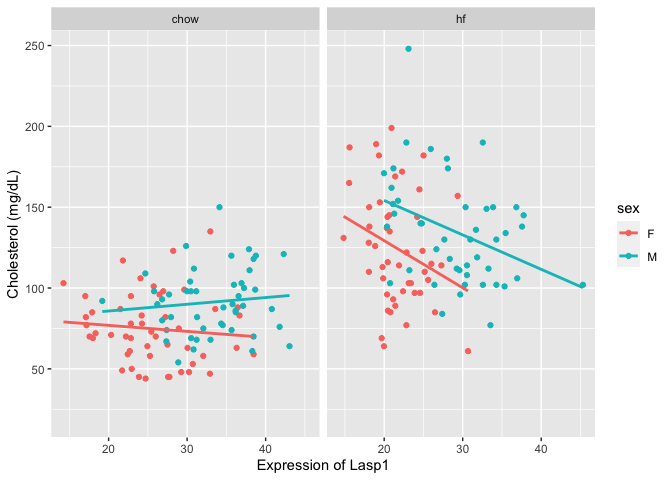
\includegraphics{figures/Lasp1-associations-1.png}

\begin{Shaded}
\begin{Highlighting}[]
\NormalTok{expression.data }\SpecialCharTok{\%\textgreater{}\%}
  \FunctionTok{filter}\NormalTok{(ENSEMBL.ID }\SpecialCharTok{==}\NormalTok{ gene.ens) }\SpecialCharTok{\%\textgreater{}\%}
  \FunctionTok{pivot\_longer}\NormalTok{(}\AttributeTok{cols=}\FunctionTok{c}\NormalTok{(}\FunctionTok{starts\_with}\NormalTok{(}\StringTok{\textquotesingle{}F\textquotesingle{}}\NormalTok{),}
                      \FunctionTok{starts\_with}\NormalTok{(}\StringTok{\textquotesingle{}M\textquotesingle{}}\NormalTok{)),}
               \AttributeTok{names\_to=}\StringTok{\textquotesingle{}mouse.id\textquotesingle{}}\NormalTok{,}
               \AttributeTok{values\_to=}\StringTok{\textquotesingle{}expression\textquotesingle{}}\NormalTok{) }\SpecialCharTok{\%\textgreater{}\%}
  \FunctionTok{full\_join}\NormalTok{(phenotype.data,}\AttributeTok{by=}\StringTok{\textquotesingle{}mouse.id\textquotesingle{}}\NormalTok{) }\SpecialCharTok{\%\textgreater{}\%}
  \FunctionTok{filter}\NormalTok{(}\SpecialCharTok{!}\FunctionTok{is.na}\NormalTok{(diet)) }\SpecialCharTok{\%\textgreater{}\%}
  \FunctionTok{filter}\NormalTok{(diet}\SpecialCharTok{==}\StringTok{\textquotesingle{}chow\textquotesingle{}}\NormalTok{) }\OtherTok{{-}\textgreater{}}\NormalTok{ gene.chow.data}

\FunctionTok{lm}\NormalTok{(}\AttributeTok{data=}\NormalTok{gene.chow.data, chol2 }\SpecialCharTok{\textasciitilde{}}\NormalTok{ expression }\SpecialCharTok{+}\NormalTok{ sex) }\SpecialCharTok{\%\textgreater{}\%}
\NormalTok{  tidy }\SpecialCharTok{\%\textgreater{}\%}
  \FunctionTok{kable}\NormalTok{(}\AttributeTok{caption=}\StringTok{"Summary associations of Lasp1 and cholesterol on chow"}\NormalTok{)}
\end{Highlighting}
\end{Shaded}

\begin{longtable}[]{@{}lrrrr@{}}
\caption{Summary associations of Lasp1 and cholesterol on
chow}\tabularnewline
\toprule()
term & estimate & std.error & statistic & p.value \\
\midrule()
\endfirsthead
\toprule()
term & estimate & std.error & statistic & p.value \\
\midrule()
\endhead
(Intercept) & 75.387 & 10.515 & 7.170 & 0.000 \\
expression & -0.022 & 0.394 & -0.056 & 0.955 \\
sexM & 16.663 & 5.225 & 3.189 & 0.002 \\
\bottomrule()
\end{longtable}

\begin{Shaded}
\begin{Highlighting}[]
\FunctionTok{library}\NormalTok{(MASS)}
\FunctionTok{rlm}\NormalTok{(}\AttributeTok{data=}\NormalTok{gene.chow.data, chol2 }\SpecialCharTok{\textasciitilde{}}\NormalTok{ expression }\SpecialCharTok{+}\NormalTok{ sex) }\SpecialCharTok{\%\textgreater{}\%}
\NormalTok{  tidy }\SpecialCharTok{\%\textgreater{}\%}
  \FunctionTok{kable}\NormalTok{(}\AttributeTok{caption=}\StringTok{"Summary associations of Lasp1 and cholesterol on chow, using robust linear models"}\NormalTok{)}
\end{Highlighting}
\end{Shaded}

\begin{longtable}[]{@{}lrrr@{}}
\caption{Summary associations of Lasp1 and cholesterol on chow, using
robust linear models}\tabularnewline
\toprule()
term & estimate & std.error & statistic \\
\midrule()
\endfirsthead
\toprule()
term & estimate & std.error & statistic \\
\midrule()
\endhead
(Intercept) & 77.547 & 11.157 & 6.951 \\
expression & -0.167 & 0.418 & -0.399 \\
sexM & 18.260 & 5.544 & 3.294 \\
\bottomrule()
\end{longtable}

\begin{Shaded}
\begin{Highlighting}[]
\NormalTok{expression.data }\SpecialCharTok{\%\textgreater{}\%}
  \FunctionTok{filter}\NormalTok{(ENSEMBL.ID }\SpecialCharTok{==}\NormalTok{ gene.ens) }\SpecialCharTok{\%\textgreater{}\%}
  \FunctionTok{pivot\_longer}\NormalTok{(}\AttributeTok{cols=}\FunctionTok{c}\NormalTok{(}\FunctionTok{starts\_with}\NormalTok{(}\StringTok{\textquotesingle{}F\textquotesingle{}}\NormalTok{),}
                      \FunctionTok{starts\_with}\NormalTok{(}\StringTok{\textquotesingle{}M\textquotesingle{}}\NormalTok{)),}
               \AttributeTok{names\_to=}\StringTok{\textquotesingle{}mouse.id\textquotesingle{}}\NormalTok{,}
               \AttributeTok{values\_to=}\StringTok{\textquotesingle{}expression\textquotesingle{}}\NormalTok{) }\SpecialCharTok{\%\textgreater{}\%}
  \FunctionTok{full\_join}\NormalTok{(phenotype.data,}\AttributeTok{by=}\StringTok{\textquotesingle{}mouse.id\textquotesingle{}}\NormalTok{) }\SpecialCharTok{\%\textgreater{}\%}
  \FunctionTok{filter}\NormalTok{(}\SpecialCharTok{!}\FunctionTok{is.na}\NormalTok{(diet)) }\OtherTok{{-}\textgreater{}}\NormalTok{ gene.hf.data}

\FunctionTok{lm}\NormalTok{(}\AttributeTok{data=}\NormalTok{gene.hf.data, chol2 }\SpecialCharTok{\textasciitilde{}}\NormalTok{ expression }\SpecialCharTok{+}\NormalTok{ sex) }\SpecialCharTok{\%\textgreater{}\%}
\NormalTok{  tidy }\SpecialCharTok{\%\textgreater{}\%}
  \FunctionTok{kable}\NormalTok{(}\AttributeTok{caption=}\StringTok{"Summary associations of Lasp1 and cholesterol on HFD"}\NormalTok{)}
\end{Highlighting}
\end{Shaded}

\begin{longtable}[]{@{}lrrrr@{}}
\caption{Summary associations of Lasp1 and cholesterol on
HFD}\tabularnewline
\toprule()
term & estimate & std.error & statistic & p.value \\
\midrule()
\endfirsthead
\toprule()
term & estimate & std.error & statistic & p.value \\
\midrule()
\endhead
(Intercept) & 156.11 & 11.333 & 13.78 & 0 \\
expression & -2.42 & 0.455 & -5.31 & 0 \\
sexM & 31.96 & 6.032 & 5.30 & 0 \\
\bottomrule()
\end{longtable}

\hypertarget{session-information}{%
\section{Session Information}\label{session-information}}

\begin{Shaded}
\begin{Highlighting}[]
\FunctionTok{sessionInfo}\NormalTok{()}
\end{Highlighting}
\end{Shaded}

\begin{verbatim}
## R version 4.2.2 (2022-10-31)
## Platform: x86_64-apple-darwin17.0 (64-bit)
## Running under: macOS Big Sur ... 10.16
## 
## Matrix products: default
## BLAS:   /Library/Frameworks/R.framework/Versions/4.2/Resources/lib/libRblas.0.dylib
## LAPACK: /Library/Frameworks/R.framework/Versions/4.2/Resources/lib/libRlapack.dylib
## 
## locale:
## [1] en_US.UTF-8/en_US.UTF-8/en_US.UTF-8/C/en_US.UTF-8/en_US.UTF-8
## 
## attached base packages:
## [1] stats4    stats     graphics  grDevices utils     datasets  methods  
## [8] base     
## 
## other attached packages:
##  [1] MASS_7.3-58.1         ggupset_0.3.0         enrichplot_1.16.2    
##  [4] clusterProfiler_4.4.4 ggrepel_0.9.2         ggplot2_3.4.0        
##  [7] venneuler_1.1-3       rJava_1.0-6           purrr_1.0.1          
## [10] org.Mm.eg.db_3.15.0   AnnotationDbi_1.58.0  IRanges_2.30.1       
## [13] S4Vectors_0.34.0      Biobase_2.56.0        BiocGenerics_0.42.0  
## [16] broom_1.0.2           readr_2.1.3           dplyr_1.0.10         
## [19] tidyr_1.2.1           knitr_1.41           
## 
## loaded via a namespace (and not attached):
##   [1] fgsea_1.22.0           colorspace_2.0-3       ggtree_3.4.4          
##   [4] ellipsis_0.3.2         qvalue_2.28.0          XVector_0.36.0        
##   [7] aplot_0.1.9            rstudioapi_0.14        farver_2.1.1          
##  [10] graphlayouts_0.8.4     bit64_4.0.5            scatterpie_0.1.8      
##  [13] fansi_1.0.3            codetools_0.2-18       splines_4.2.2         
##  [16] cachem_1.0.6           GOSemSim_2.22.0        polyclip_1.10-4       
##  [19] jsonlite_1.8.4         GO.db_3.15.0           png_0.1-8             
##  [22] ggforce_0.4.1          compiler_4.2.2         httr_1.4.4            
##  [25] backports_1.4.1        lazyeval_0.2.2         assertthat_0.2.1      
##  [28] Matrix_1.5-3           fastmap_1.1.0          cli_3.6.0             
##  [31] tweenr_2.0.2           htmltools_0.5.4        tools_4.2.2           
##  [34] igraph_1.3.5           gtable_0.3.1           glue_1.6.2            
##  [37] GenomeInfoDbData_1.2.8 reshape2_1.4.4         DO.db_2.9             
##  [40] fastmatch_1.1-3        Rcpp_1.0.9             vctrs_0.5.1           
##  [43] Biostrings_2.64.1      ape_5.6-2              nlme_3.1-161          
##  [46] ggraph_2.1.0           xfun_0.36              stringr_1.5.0         
##  [49] lifecycle_1.0.3        DOSE_3.22.1            zlibbioc_1.42.0       
##  [52] scales_1.2.1           tidygraph_1.2.2        vroom_1.6.0           
##  [55] hms_1.1.2              parallel_4.2.2         RColorBrewer_1.1-3    
##  [58] yaml_2.3.6             memoise_2.0.1          gridExtra_2.3         
##  [61] downloader_0.4         ggfun_0.0.9            yulab.utils_0.0.6     
##  [64] stringi_1.7.12         RSQLite_2.2.20         highr_0.10            
##  [67] tidytree_0.4.2         BiocParallel_1.30.4    GenomeInfoDb_1.32.4   
##  [70] rlang_1.0.6            pkgconfig_2.0.3        bitops_1.0-7          
##  [73] evaluate_0.19          lattice_0.20-45        treeio_1.20.2         
##  [76] patchwork_1.1.2        labeling_0.4.2         shadowtext_0.1.2      
##  [79] bit_4.0.5              tidyselect_1.2.0       plyr_1.8.8            
##  [82] magrittr_2.0.3         R6_2.5.1               magick_2.7.3          
##  [85] generics_0.1.3         DBI_1.1.3              pillar_1.8.1          
##  [88] withr_2.5.0            mgcv_1.8-41            KEGGREST_1.36.3       
##  [91] RCurl_1.98-1.9         tibble_3.1.8           crayon_1.5.2          
##  [94] utf8_1.2.2             tzdb_0.3.0             rmarkdown_2.19        
##  [97] viridis_0.6.2          grid_4.2.2             data.table_1.14.6     
## [100] blob_1.2.3             digest_0.6.31          gridGraphics_0.5-1    
## [103] munsell_0.5.0          viridisLite_0.4.1      ggplotify_0.1.0
\end{verbatim}

\end{document}
